Reproducibility without a mandate: computational reproduction and multiverse analysis of exercise, rehabilitation and physiotherapy trials with publicly deposited individual participant data. Jürgen Degenfellner, ZHAW. Generated from the project files on 2026-09-15.

\section{Text S1. Transparency statement for secondary data analysis (after van den Akker et al.~2021)}\label{text-s1.-transparency-statement-for-secondary-data-analysis-after-van-den-akker-et-al.-2021}

\textbf{Prior knowledge of the data.} All 48 deposits were downloaded on 28 August 2026 and inspected for file structure before the grid of decision nodes was written on the same day. No specification had been computed at that point. The published analyses were extracted from the papers on 12 September 2026, and the mapping rules of Methods 2.3 were fixed after that extraction.

\textbf{Order of analyses.} First complete multiverse run: 28 August 2026, with the ad hoc mapping (registry v1). Rule-based mapping (registry v2) and rerun: 12 September 2026. Statistical review and corrections (pooled within-group denominator, reproduction rule, multiple imputation): 12 September 2026. Adversarial review, reclassification of outlier rules, addition of the strict grid, long-format baseline correction, refit of the published models: 13 September 2026. Displacement analysis: 13 September 2026.

\textbf{Decisions made after seeing results.} Outlier rules were moved from the core grid to a sensitivity arm after a winsorising rule on a bounded outcome had produced a range of 1.08 standard deviations. The strict grid was added after the first run showed that in most trials only baseline handling could vary. The core grid was renamed from principled to estimand-preserving after the precision criterion had been applied to baseline handling. The reproduction rule (2\% and 10\% relative difference) was fixed before any computation. An absolute criterion introduced on 12 September was withdrawn on 13 September and the prespecified rule reinstated, with the absolute difference reported without threshold.

\textbf{Registry v1 versus v2.} Table S2 lists both mappings, Table S7 the effect of v1 on the results. The sign of the median effect reversed in 7 of 16 trials.

\textbf{Coders.} One coder to date. A second, blind coding is planned and its agreement will be reported.

\section{Table S1. Exclusions at manual assessment (n = 32)}\label{table-s1.-exclusions-at-manual-assessment-n-32}

{
\begin{longtable}[]{@{}
  >{\raggedright\arraybackslash}p{(\linewidth - 6\tabcolsep) * \real{0.2500}}
  >{\raggedright\arraybackslash}p{(\linewidth - 6\tabcolsep) * \real{0.2500}}
  >{\raggedright\arraybackslash}p{(\linewidth - 6\tabcolsep) * \real{0.2500}}
  >{\raggedright\arraybackslash}p{(\linewidth - 6\tabcolsep) * \real{0.2500}}@{}}
\toprule\noalign{}
\begin{minipage}[b]{\linewidth}\raggedright
study\_id
\end{minipage} & \begin{minipage}[b]{\linewidth}\raggedright
category
\end{minipage} & \begin{minipage}[b]{\linewidth}\raggedright
reason\_code
\end{minipage} & \begin{minipage}[b]{\linewidth}\raggedright
reason
\end{minipage} \\
\midrule\noalign{}
\endhead
\bottomrule\noalign{}
\endlastfoot
2016\_early-sitting-in-ischemic-stroke-patients-sevel & design & binary\_outcome & Primaeres Outcome ist der Anteil mit modifiziertem Rankin-Score 0-2 und damit binaer; das Gitter ist fuer stetige Outcomes gebaut \\
2017\_predicting-outcome-in-frozen-shoulder-shoulder-c & duplicate & duplicate\_data & Nutzt denselben Datensatz wie die Adhesive-Capsulitis-Studie (106 Zeilen, Group 1/2/3, identische SPADI-Spalten); Doppelzaehlung \\
2020\_an-age-adapted-plyometric-exercise-program-impro & design & feasibility\_primary & Machbarkeitsstudie; primaerer Endpunkt ist die Durchfuehrbarkeit des Programms \\
2021\_home-based-exercise-for-people-living-with-frail & design & feasibility\_primary & Primaere Endpunkte sind Eignung, Rekrutierung, Adhaerenz und Abbruchquote; kein Effektschaetzer \\
2022\_dependence-of-learning-outcomes-in-flipped-and-l & design & not\_clinical & Lehrforschung zu Unterrichtsformaten; keine klinische Studie an Patienten \\
2022\_a-comparison-of-psychological-characteristics-in & design & not\_rct & Querschnitts- bzw. Kohortenvergleich psychologischer Merkmale; keine randomisierte Intervention \\
2025\_subphenotypic-classification-of-covid-19-survivo & duplicate & duplicate\_data & Latent-Class-Sekundaeranalyse desselben TERECO-Datensatzes (119 Zeilen, group\_randomized, SF12-Spalten) \\
2025\_isoenergetic-pre-exercise-meals-varying-in-carbo & design & crossover\_design & Crossover-Design; das Gitter unterstellt parallele Gruppen und wuerde die Within-Person-Struktur ignorieren \\
2021\_impact-of-assessment-and-intervention-by-a-healt & data & outcome\_not\_identifiable & Primaeres Outcome laut Abstract ED length of stay; im Deposit ist keine Spalte eindeutig als solche erkennbar \\
2024\_effects-of-anodal-tdcs-on-resting-state-eeg-powe & data & outcome\_data\_not\_tabular & Die Tabellendatei enthaelt nur Basischarakteristika; die EEG-Outcomes liegen in 7z-Archiven \\
2022\_influence-of-the-statistical-significance-of-res & design & not\_clinical & Leserstudie: Wie interpretieren Leser Abstracts mit und ohne Spin; keine Intervention an Patienten \\
2021\_the-impact-of-a-physician-s-recommendation-and-g & design & not\_clinical & Qualtrics-Vignettenbefragung zu Arztempfehlung und Geschlecht; keine klinische Intervention \\
2021\_effect-of-an-inverted-seated-position-with-upper & design & crossover\_design & Vier Bedingungen je Person mit Rest/Pre/Post; Crossover, keine parallelen Gruppen \\
2023\_a-clinical-model-to-predict-the-progression-of-k & design & not\_rct & Prognosemodell fuer den Verlauf der Gonarthrose; keine Randomisierung \\
2025\_comparative-effects-of-combined-aerobic-and-resi & data & no\_ipd & Das Deposit enthaelt nur eine Ergebnistabelle mit Gruppendifferenzen und CIs, keine Individualdaten \\
2025\_comparing-structured-note-taking-and-multiple-ch & design & not\_clinical & Lehrforschung zu Notiztechniken; keine klinische Studie \\
2026\_effects-of-modest-carbohydrate-energy-supplement & design & crossover\_design & Jede Person erhaelt beide Supplemente (Supplement\_1 und Supplement\_2 in allen 20 Zeilen belegt, je 10 C und 10 P); Crossover statt paralleler Gruppen \\
2026\_preliminary-efficacy-of-cognitive-multisensory-r & data & arm\_not\_in\_data & Das Paper randomisiert in sofortige CMR (Gruppe A) und Beobachtung (Gruppe B), im Deposit gibt es aber keine Gruppenspalte \\
2025\_time-restricted-eating-without-exercise-enhances & design & crossover\_design & Drei Phasen je Person (Phase 1, 2, 3) ohne Gruppenvariable; Within-Person-Design \\
2024\_eight-weeks-of-high-intensity-interval-training & data & file\_not\_readable & Die beiden CSV-Dateien im Deposit lassen sich nicht als Tabelle einlesen (inkonsistente Spaltenzahl) \\
2022\_the-effect-of-mindfulness-on-the-inflammatory-ps & data & no\_data\_in\_deposit & Das im Availability-Statement verlinkte Archiv enthaelt ausschliesslich eine README.md und keine Daten \\
2025\_a-sensor-augmented-telerehabilitation-system-for & data & outcome\_data\_not\_tabular & Das Deposit enthaelt nur EMG- und IMU-Rohsignale als NumPy-Arrays je Proband und Versuch, keine Outcome-Tabelle \\
2026\_effects-of-low-load-blood-flow-restriction-train & data & arm\_not\_in\_data & Die Daten liegen als extdata eines R-Pakets in Parquet- und Excel-Dateien; in der Kontraktilitaetstabelle fehlt eine Gruppenvariable \\
2023\_the-effects-of-creatine-supplementation-on-cogni & design & crossover\_design & Supplement-Reihenfolge je Person (order\_supplement, guess\_first\_supplement); Crossover statt paralleler Gruppen, dazu vier getrennte Testdateien \\
2025\_the-effect-of-proximity-to-failure-on-perceptual & design & within\_person\_design & Beide Gliedmassen je Person erhalten unterschiedliche Protokolle (FAIL gegen RIR); Within-Person-Design \\
2026\_anatomy-of-a-failure-a-retrospective-evaluation & data & arm\_not\_in\_data & Retrospektive Auswertung; die Spalte CONDITION kodiert Messzeitpunkte (1w, 1m, 3m, 6m, 12m), eine Gruppenvariable ist nicht auffindbar \\
2025\_lengthened-partial-repetitions-elicit-similar-mu & design & within\_person\_design & Beide Arme je Person erhalten unterschiedliche Protokolle (pROM/fROM kontralateral); kein Parallelgruppen-Kontrollarm. Gleiche Regel wie bei der Proximity-to-Fa \\
2024\_pilot-randomized-controlled-trial-of-i-lymfit-i & design & feasibility\_primary & Pilot-Machbarkeits-RCT (n=26); primaeres Ziel sind Feasibility-Benchmarks, kein Wirksamkeits-Primaeroutcome. Gleiche Regel wie bei den zwei anderen Machbarkeits \\
2022\_understanding-how-individualised-physiotherapy-o & no\_estimate & no\_group\_estimate & Explorative Netzwerkanalyse (Mixed Graphical Model) ueber 10 ODI-Items einer Sekundaeranalyse des STOPS-Trials; kein Gruppendifferenz-Schaetzer, kein primaeres \\
2025\_effects-of-an-aquatic-protocol-on-electromyograp & data & outcome\_not\_identifiable & Kein primaeres Outcome deklariert; Abstract nennt zuerst EMG-Aktivierung gemittelt ueber 4 Muskeln, im Deposit nur Einzelmuskel-Spalten mit unbeschrifteten Suff \\
2015\_a-12-week-exercise-program-for-pregnant-women-wi & data & outcome\_timepoint\_not\_in\_deposit & Primaeres Outcome (nach dokumentiertem Outcome-Switching) ist MVPA in Bouts bei 36 SSW; das Deposit enthaelt nur v1 (14 SSW) und v2 (28 SSW). Regel: publizierte \\
2026\_changes-in-repetitive-negative-thinking-and-stre & no\_estimate & secondary\_analysis\_no\_estimate & Mediationsanalyse (SEM) des ImPuls-RCT (Wolf et al.~2024, Lancet Psychiatry); kein eigener Gruppenvergleichs-Schaetzer; Primaerbericht liegt anderswo \\
\end{longtable}
}

\section{Table S2. Trial registry, version 2 (rule-based) against version 1 (ad hoc)}\label{table-s2.-trial-registry-version-2-rule-based-against-version-1-ad-hoc}

{
\begin{longtable}[]{@{}
  >{\raggedright\arraybackslash}p{(\linewidth - 16\tabcolsep) * \real{0.1111}}
  >{\raggedright\arraybackslash}p{(\linewidth - 16\tabcolsep) * \real{0.1111}}
  >{\raggedright\arraybackslash}p{(\linewidth - 16\tabcolsep) * \real{0.1111}}
  >{\raggedright\arraybackslash}p{(\linewidth - 16\tabcolsep) * \real{0.1111}}
  >{\raggedright\arraybackslash}p{(\linewidth - 16\tabcolsep) * \real{0.1111}}
  >{\raggedright\arraybackslash}p{(\linewidth - 16\tabcolsep) * \real{0.1111}}
  >{\raggedright\arraybackslash}p{(\linewidth - 16\tabcolsep) * \real{0.1111}}
  >{\raggedright\arraybackslash}p{(\linewidth - 16\tabcolsep) * \real{0.1111}}
  >{\raggedright\arraybackslash}p{(\linewidth - 16\tabcolsep) * \real{0.1111}}@{}}
\toprule\noalign{}
\begin{minipage}[b]{\linewidth}\raggedright
study\_id
\end{minipage} & \begin{minipage}[b]{\linewidth}\raggedright
report\_type
\end{minipage} & \begin{minipage}[b]{\linewidth}\raggedright
outcome\_v2
\end{minipage} & \begin{minipage}[b]{\linewidth}\raggedright
outcome\_v1
\end{minipage} & \begin{minipage}[b]{\linewidth}\raggedright
control\_v2
\end{minipage} & \begin{minipage}[b]{\linewidth}\raggedright
control\_v1
\end{minipage} & \begin{minipage}[b]{\linewidth}\raggedright
covariates\_v2
\end{minipage} & \begin{minipage}[b]{\linewidth}\raggedright
covariates\_v1
\end{minipage} & \begin{minipage}[b]{\linewidth}\raggedright
primary\_declared
\end{minipage} \\
\midrule\noalign{}
\endhead
\bottomrule\noalign{}
\endlastfoot
physiofeedback\_PMC12821712 & secondary & AP\_RMS & AP\_RMS & Control & Control & Age,BMI,Gender,Race & Age,BMI,Gender,Race & secondary\_report \\
mulligan\_PMC13092435 & primary & NPRS2 & NPRS2 & 3 & 1 & & Age,Gender & registration \\
lytras\_fms\_PMC12942207 & primary & NRPSLBPpost & NRPSLBPpost & 2 & 1 & & Age,Gender,BMI & registration \\
clusterset\_PMC13140343 & primary & 1RM & CMJ\_mean & TS & TS & Sex & Age,Sex & sample\_size \\
tereco\_PMC8318721 & primary & X\_6MWD2 & X\_6MWD2 & 2 & 1 & & & registration \\
spadi\_PMC4880881 & primary & SPADI8wks & SPADItot4wks & 3 & 1 & & & registration \\
tscs\_PMC13085461 & primary & BBS\_Post & BBS\_Post & 2 & 1 & & Age,BMI & registration \\
tdcs\_PMC13257960 & secondary & CAR\_post\_all & CAR\_post\_all & 2 & 1 & & age,BMI & secondary\_report \\
etip\_PMC6886967 & secondary & Post\_PGWB & EPDS\_total & 2 & 1 & & Pre\_preg\_BMI & secondary\_report \\
phosphatidic\_PMC4891923 & primary & LBM2 & LBM2 & 2 & 1 & & Age,Sex & none \\
facial\_PMC11164989 & primary & T3 & VM2 & 2 & 1 & & Age & registration \\
gainingmore\_PMC10809978 & primary & RF50Post & RF50Post & 2 & 1 & & SEX & none \\
etre\_PMC11945196 & primary & Weight & Weight & Control & Control & & & paper \\
creatine\_PMC11944689 & primary & dxa\_leanmass\_kg\_post\_1 & legs\_post1 & Control & Control & & sex & registration \\
free\_PMC6733445 & primary & rmdq\_tot & rmdq\_tot & Control & Control & agegp\_w0 & & registration \\
mallorca\_PMC8198819 & secondary & edimburgtotal & edimburgtotal & C & C & & & secondary\_report \\
\end{longtable}
}

\section{Table S3. Summary measures per trial and grid}\label{table-s3.-summary-measures-per-trial-and-grid}

grid\_type: principled = estimand-preserving; strict = baseline handling fixed to analysis of covariance; defensible = Type E and N nodes; outlier\_arm = sensitivity arm.

{
\begin{longtable}[]{@{}
  >{\raggedright\arraybackslash}p{(\linewidth - 20\tabcolsep) * \real{0.0909}}
  >{\raggedright\arraybackslash}p{(\linewidth - 20\tabcolsep) * \real{0.0909}}
  >{\raggedright\arraybackslash}p{(\linewidth - 20\tabcolsep) * \real{0.0909}}
  >{\raggedright\arraybackslash}p{(\linewidth - 20\tabcolsep) * \real{0.0909}}
  >{\raggedright\arraybackslash}p{(\linewidth - 20\tabcolsep) * \real{0.0909}}
  >{\raggedright\arraybackslash}p{(\linewidth - 20\tabcolsep) * \real{0.0909}}
  >{\raggedright\arraybackslash}p{(\linewidth - 20\tabcolsep) * \real{0.0909}}
  >{\raggedright\arraybackslash}p{(\linewidth - 20\tabcolsep) * \real{0.0909}}
  >{\raggedright\arraybackslash}p{(\linewidth - 20\tabcolsep) * \real{0.0909}}
  >{\raggedright\arraybackslash}p{(\linewidth - 20\tabcolsep) * \real{0.0909}}
  >{\raggedright\arraybackslash}p{(\linewidth - 20\tabcolsep) * \real{0.0909}}@{}}
\toprule\noalign{}
\begin{minipage}[b]{\linewidth}\raggedright
study\_id
\end{minipage} & \begin{minipage}[b]{\linewidth}\raggedright
grid\_type
\end{minipage} & \begin{minipage}[b]{\linewidth}\raggedright
n\_spec
\end{minipage} & \begin{minipage}[b]{\linewidth}\raggedright
n
\end{minipage} & \begin{minipage}[b]{\linewidth}\raggedright
d\_median
\end{minipage} & \begin{minipage}[b]{\linewidth}\raggedright
d\_q25
\end{minipage} & \begin{minipage}[b]{\linewidth}\raggedright
d\_q75
\end{minipage} & \begin{minipage}[b]{\linewidth}\raggedright
d\_min
\end{minipage} & \begin{minipage}[b]{\linewidth}\raggedright
d\_max
\end{minipage} & \begin{minipage}[b]{\linewidth}\raggedright
share\_same\_sign
\end{minipage} & \begin{minipage}[b]{\linewidth}\raggedright
s\_median
\end{minipage} \\
\midrule\noalign{}
\endhead
\bottomrule\noalign{}
\endlastfoot
clusterset\_PMC13140343 & defensible & 36 & 36 & 0.0644 & 0.0559 & 0.157 & 0.0528 & 0.179 & 1 & 1.49 \\
clusterset\_PMC13140343 & outlier\_arm & 18 & 36 & 0.0593 & 0.0542 & 0.155 & 0.0528 & 0.171 & 1 & 1.52 \\
clusterset\_PMC13140343 & principled & 18 & 36 & 0.0593 & 0.0542 & 0.155 & 0.0528 & 0.171 & 1 & 1.52 \\
clusterset\_PMC13140343 & strict & 6 & 36 & 0.0583 & 0.0528 & 0.0637 & 0.0528 & 0.0637 & 1 & 1.55 \\
creatine\_PMC11944689 & defensible & 48 & 64 & 0.0431 & 0.0414 & 0.196 & 0.0163 & 0.28 & 1 & 3.18 \\
creatine\_PMC11944689 & outlier\_arm & 9 & 63 & 0.0446 & 0.0439 & 0.256 & 0.0439 & 0.256 & 1 & 5.16 \\
creatine\_PMC11944689 & principled & 9 & 63 & 0.0446 & 0.0439 & 0.256 & 0.0439 & 0.256 & 1 & 5.16 \\
creatine\_PMC11944689 & strict & 3 & 63 & 0.0439 & 0.0439 & 0.0439 & 0.0439 & 0.0439 & 1 & 5.14 \\
etip\_PMC6886967 & defensible & 48 & 91 & 0.132 & 0.0802 & 0.185 & -0.0161 & 0.254 & 0.938 & 0.98 \\
etip\_PMC6886967 & outlier\_arm & 30 & 59 & 0.227 & 0.192 & 0.275 & 0.0447 & 0.289 & 1 & 1.6 \\
etip\_PMC6886967 & principled & 9 & 59 & 0.192 & 0.0447 & 0.254 & 0.0447 & 0.254 & 1 & 1.23 \\
etip\_PMC6886967 & strict & 3 & 59 & 0.192 & 0.192 & 0.192 & 0.192 & 0.192 & 1 & 1.22 \\
etre\_PMC11945196 & defensible & 18 & 16 & -0.916 & -1.24 & -0.887 & -1.26 & -0.874 & 1 & 9.41 \\
etre\_PMC11945196 & outlier\_arm & 9 & 16 & -0.903 & -1.24 & -0.874 & -1.24 & -0.874 & 1 & 9.7 \\
etre\_PMC11945196 & principled & 9 & 16 & -0.903 & -1.24 & -0.874 & -1.24 & -0.874 & 1 & 9.7 \\
etre\_PMC11945196 & strict & 3 & 16 & -0.874 & -0.874 & -0.874 & -0.874 & -0.874 & 1 & 8.97 \\
facial\_PMC11164989 & defensible & 30 & 24 & 1.51 & 1.45 & 1.55 & 1.35 & 1.6 & 1 & 9.53 \\
facial\_PMC11164989 & outlier\_arm & 16 & 23 & 1.49 & 1.45 & 1.51 & 1.44 & 1.55 & 1 & 9.57 \\
facial\_PMC11164989 & principled & 9 & 23 & 1.49 & 1.45 & 1.55 & 1.45 & 1.55 & 1 & 9.64 \\
facial\_PMC11164989 & strict & 3 & 23 & 1.49 & 1.49 & 1.49 & 1.49 & 1.49 & 1 & 10.6 \\
free\_PMC6733445 & defensible & 96 & 226 & 0.092 & 0.0752 & 0.0977 & -0.0605 & 0.137 & 0.948 & 0.79 \\
free\_PMC6733445 & outlier\_arm & 219 & 214 & 0.0549 & 0.0203 & 0.085 & -0.0309 & 0.117 & 0.913 & 0.424 \\
free\_PMC6733445 & principled & 35 & 214 & 0.0911 & 0.0753 & 0.0952 & 0.0562 & 0.117 & 1 & 0.797 \\
free\_PMC6733445 & strict & 12 & 214 & 0.0911 & 0.0847 & 0.0936 & 0.0753 & 0.105 & 1 & 0.886 \\
gainingmore\_PMC10809978 & defensible & 18 & 39 & -0.102 & -0.468 & -0.06 & -0.499 & -0.0423 & 1 & 1.07 \\
gainingmore\_PMC10809978 & outlier\_arm & 9 & 39 & -0.0901 & -0.468 & -0.06 & -0.468 & -0.06 & 1 & 0.956 \\
gainingmore\_PMC10809978 & principled & 9 & 39 & -0.0901 & -0.468 & -0.06 & -0.468 & -0.06 & 1 & 0.956 \\
gainingmore\_PMC10809978 & strict & 3 & 39 & -0.0901 & -0.0901 & -0.0901 & -0.0901 & -0.0901 & 1 & 0.956 \\
lytras\_fms\_PMC12942207 & defensible & 9 & 40 & -0.884 & -1.01 & -0.785 & -1.01 & -0.785 & 1 & 7.35 \\
lytras\_fms\_PMC12942207 & outlier\_arm & 9 & 40 & -0.884 & -1.01 & -0.785 & -1.01 & -0.785 & 1 & 7.35 \\
lytras\_fms\_PMC12942207 & principled & 9 & 40 & -0.884 & -1.01 & -0.785 & -1.01 & -0.785 & 1 & 7.35 \\
lytras\_fms\_PMC12942207 & strict & 3 & 40 & -0.884 & -0.884 & -0.884 & -0.884 & -0.884 & 1 & 7.7 \\
mallorca\_PMC8198819 & defensible & 10 & 294 & -0.301 & -0.313 & -0.295 & -0.315 & -0.281 & 1 & 5.82 \\
mallorca\_PMC8198819 & outlier\_arm & 19 & 263 & -0.287 & -0.304 & -0.244 & -0.315 & -0.236 & 1 & 6.36 \\
mallorca\_PMC8198819 & principled & 3 & 263 & -0.315 & -0.315 & -0.315 & -0.315 & -0.315 & 1 & 6.48 \\
mallorca\_PMC8198819 & strict & 3 & 263 & -0.315 & -0.315 & -0.315 & -0.315 & -0.315 & 1 & 6.48 \\
mulligan\_PMC13092435 & defensible & 18 & 29 & -0.325 & -0.329 & -0.22 & -0.411 & -0.117 & 1 & 1.52 \\
mulligan\_PMC13092435 & outlier\_arm & 9 & 29 & -0.22 & -0.32 & -0.117 & -0.32 & -0.117 & 1 & 1.03 \\
mulligan\_PMC13092435 & principled & 9 & 29 & -0.22 & -0.32 & -0.117 & -0.32 & -0.117 & 1 & 1.03 \\
mulligan\_PMC13092435 & strict & 3 & 29 & -0.22 & -0.22 & -0.22 & -0.22 & -0.22 & 1 & 1.03 \\
phosphatidic\_PMC4891923 & defensible & 18 & 18 & 0.101 & 0.0637 & 0.105 & 0.0562 & 0.106 & 1 & 4.01 \\
phosphatidic\_PMC4891923 & outlier\_arm & 9 & 18 & 0.105 & 0.0637 & 0.106 & 0.0637 & 0.106 & 1 & 3.83 \\
phosphatidic\_PMC4891923 & principled & 9 & 18 & 0.105 & 0.0637 & 0.106 & 0.0637 & 0.106 & 1 & 3.83 \\
phosphatidic\_PMC4891923 & strict & 3 & 18 & 0.106 & 0.106 & 0.106 & 0.106 & 0.106 & 1 & 4.41 \\
physiofeedback\_PMC12821712 & defensible & 45 & 276 & 0.0744 & 0.0493 & 0.108 & -0.0194 & 0.141 & 0.956 & 0.762 \\
physiofeedback\_PMC12821712 & outlier\_arm & 157 & 276 & 0.0913 & 0.0704 & 0.108 & 0.0222 & 0.141 & 1 & 1.13 \\
physiofeedback\_PMC12821712 & principled & 23 & 276 & 0.108 & 0.0666 & 0.133 & 0.0493 & 0.141 & 1 & 1.38 \\
physiofeedback\_PMC12821712 & strict & 8 & 276 & 0.114 & 0.108 & 0.133 & 0.0899 & 0.133 & 1 & 1.51 \\
spadi\_PMC4880881 & defensible & 24 & 72 & -0.952 & -0.975 & -0.91 & -1 & -0.869 & 1 & 14 \\
spadi\_PMC4880881 & outlier\_arm & 9 & 71 & -0.975 & -1 & -0.904 & -1 & -0.904 & 1 & 12.3 \\
spadi\_PMC4880881 & principled & 9 & 71 & -0.975 & -1 & -0.904 & -1 & -0.904 & 1 & 12.3 \\
spadi\_PMC4880881 & strict & 3 & 71 & -0.975 & -0.975 & -0.975 & -0.975 & -0.975 & 1 & 17.3 \\
tdcs\_PMC13257960 & defensible & 18 & 20 & 1.41 & 1.39 & 1.43 & 1.38 & 1.46 & 1 & 7.3 \\
tdcs\_PMC13257960 & outlier\_arm & 41 & 20 & 1.38 & 1.22 & 1.41 & 0.384 & 1.46 & 1 & 7.94 \\
tdcs\_PMC13257960 & principled & 9 & 20 & 1.42 & 1.41 & 1.46 & 1.41 & 1.46 & 1 & 7.47 \\
tdcs\_PMC13257960 & strict & 3 & 20 & 1.42 & 1.42 & 1.42 & 1.42 & 1.42 & 1 & 7.59 \\
tereco\_PMC8318721 & defensible & 96 & 119 & 0.758 & 0.655 & 0.808 & 0.537 & 0.917 & 1 & 16.4 \\
tereco\_PMC8318721 & outlier\_arm & 126 & 112 & 0.826 & 0.801 & 0.858 & 0.762 & 0.913 & 1 & 19.1 \\
tereco\_PMC8318721 & principled & 18 & 112 & 0.843 & 0.808 & 0.901 & 0.793 & 0.913 & 1 & 17.9 \\
tereco\_PMC8318721 & strict & 6 & 112 & 0.843 & 0.834 & 0.851 & 0.834 & 0.851 & 1 & 24.3 \\
tscs\_PMC13085461 & defensible & 18 & 20 & 1.09 & 0.976 & 1.36 & 0.975 & 1.5 & 1 & 10.8 \\
tscs\_PMC13085461 & outlier\_arm & 9 & 20 & 1.03 & 0.975 & 1.36 & 0.975 & 1.36 & 1 & 12.3 \\
tscs\_PMC13085461 & principled & 9 & 20 & 1.03 & 0.975 & 1.36 & 0.975 & 1.36 & 1 & 12.3 \\
tscs\_PMC13085461 & strict & 3 & 20 & 0.975 & 0.975 & 0.975 & 0.975 & 0.975 & 1 & 17.3 \\
\end{longtable}
}

\subsection{Table S3b. Wilson intervals for proportions and study-bootstrap intervals for medians}\label{table-s3b.-wilson-intervals-for-proportions-and-study-bootstrap-intervals-for-medians}

{
\begin{longtable}[]{@{}
  >{\raggedright\arraybackslash}p{(\linewidth - 10\tabcolsep) * \real{0.1667}}
  >{\raggedright\arraybackslash}p{(\linewidth - 10\tabcolsep) * \real{0.1667}}
  >{\raggedright\arraybackslash}p{(\linewidth - 10\tabcolsep) * \real{0.1667}}
  >{\raggedright\arraybackslash}p{(\linewidth - 10\tabcolsep) * \real{0.1667}}
  >{\raggedright\arraybackslash}p{(\linewidth - 10\tabcolsep) * \real{0.1667}}
  >{\raggedright\arraybackslash}p{(\linewidth - 10\tabcolsep) * \real{0.1667}}@{}}
\toprule\noalign{}
\begin{minipage}[b]{\linewidth}\raggedright
quantity
\end{minipage} & \begin{minipage}[b]{\linewidth}\raggedright
k
\end{minipage} & \begin{minipage}[b]{\linewidth}\raggedright
n
\end{minipage} & \begin{minipage}[b]{\linewidth}\raggedright
prop
\end{minipage} & \begin{minipage}[b]{\linewidth}\raggedright
wilson\_lo
\end{minipage} & \begin{minipage}[b]{\linewidth}\raggedright
wilson\_hi
\end{minipage} \\
\midrule\noalign{}
\endhead
\bottomrule\noalign{}
\endlastfoot
reproduced full & 11 & 12 & 0.917 & 0.646 & 0.985 \\
reproduced full or minor & 11 & 12 & 0.917 & 0.646 & 0.985 \\
published inside principled range & 9 & 11 & 0.818 & 0.523 & 0.949 \\
published inside defensible range & 11 & 12 & 0.917 & 0.646 & 0.985 \\
sign stable principled & 16 & 16 & 1 & 0.806 & 1 \\
sign stable defensible & 13 & 16 & 0.812 & 0.57 & 0.934 \\
range includes 0 principled & 0 & 16 & 0 & 0 & 0.194 \\
spec fully representable & 7 & 12 & 0.583 & 0.32 & 0.807 \\
reproduced full or minor, denominator 48 assessed RCTs & 11 & 48 & 0.229 & 0.133 & 0.365 \\
reproduced full or minor, denominator 152 with link & 11 & 152 & 0.0724 & 0.0409 & 0.125 \\
included, denominator 48 & 16 & 48 & 0.333 & 0.217 & 0.475 \\
included, denominator 152 & 16 & 152 & 0.105 & 0.0658 & 0.164 \\
\end{longtable}
}

{
\begin{longtable}[]{@{}
  >{\raggedright\arraybackslash}p{(\linewidth - 6\tabcolsep) * \real{0.2500}}
  >{\raggedright\arraybackslash}p{(\linewidth - 6\tabcolsep) * \real{0.2500}}
  >{\raggedright\arraybackslash}p{(\linewidth - 6\tabcolsep) * \real{0.2500}}
  >{\raggedright\arraybackslash}p{(\linewidth - 6\tabcolsep) * \real{0.2500}}@{}}
\toprule\noalign{}
\begin{minipage}[b]{\linewidth}\raggedright
quantity
\end{minipage} & \begin{minipage}[b]{\linewidth}\raggedright
est
\end{minipage} & \begin{minipage}[b]{\linewidth}\raggedright
boot\_lo
\end{minipage} & \begin{minipage}[b]{\linewidth}\raggedright
boot\_hi
\end{minipage} \\
\midrule\noalign{}
\endhead
\bottomrule\noalign{}
\endlastfoot
median range d, principled & 0.119 & 0.0917 & 0.212 \\
median range d, defensible & 0.239 & 0.132 & 0.322 \\
median ratio defensible/principled (finite only) & 1.35 & 1.12 & 1.52 \\
median /published d - multiverse median d/ (principled) & 0.0156 & 0.00272 & 0.0564 \\
\end{longtable}
}

\section{Table S4. Variance partition with two-way interactions, trial-by-grid combinations with at least 30 specifications}\label{table-s4.-variance-partition-with-two-way-interactions-trial-by-grid-combinations-with-at-least-30-specifications}

{
\begin{longtable}[]{@{}
  >{\raggedright\arraybackslash}p{(\linewidth - 16\tabcolsep) * \real{0.1111}}
  >{\raggedright\arraybackslash}p{(\linewidth - 16\tabcolsep) * \real{0.1111}}
  >{\raggedright\arraybackslash}p{(\linewidth - 16\tabcolsep) * \real{0.1111}}
  >{\raggedright\arraybackslash}p{(\linewidth - 16\tabcolsep) * \real{0.1111}}
  >{\raggedright\arraybackslash}p{(\linewidth - 16\tabcolsep) * \real{0.1111}}
  >{\raggedright\arraybackslash}p{(\linewidth - 16\tabcolsep) * \real{0.1111}}
  >{\raggedright\arraybackslash}p{(\linewidth - 16\tabcolsep) * \real{0.1111}}
  >{\raggedright\arraybackslash}p{(\linewidth - 16\tabcolsep) * \real{0.1111}}
  >{\raggedright\arraybackslash}p{(\linewidth - 16\tabcolsep) * \real{0.1111}}@{}}
\toprule\noalign{}
\begin{minipage}[b]{\linewidth}\raggedright
study\_id
\end{minipage} & \begin{minipage}[b]{\linewidth}\raggedright
grid\_type
\end{minipage} & \begin{minipage}[b]{\linewidth}\raggedright
n\_spec
\end{minipage} & \begin{minipage}[b]{\linewidth}\raggedright
n\_nodes
\end{minipage} & \begin{minipage}[b]{\linewidth}\raggedright
top\_additive
\end{minipage} & \begin{minipage}[b]{\linewidth}\raggedright
share\_additive
\end{minipage} & \begin{minipage}[b]{\linewidth}\raggedright
top\_interaction\_model
\end{minipage} & \begin{minipage}[b]{\linewidth}\raggedright
share\_main\_in\_interaction\_model
\end{minipage} & \begin{minipage}[b]{\linewidth}\raggedright
share\_all\_interactions
\end{minipage} \\
\midrule\noalign{}
\endhead
\bottomrule\noalign{}
\endlastfoot
free\_PMC6733445 & principled & 35 & 4 & covars & 55.3 & covars & 42.7 & 17.7 \\
physiofeedback\_PMC12821712 & defensible & 45 & 5 & transform & 43.7 & transform & 38.2 & 9.31 \\
clusterset\_PMC13140343 & defensible & 36 & 4 & baseline & 98.2 & baseline & 97.4 & 0.848 \\
tereco\_PMC8318721 & defensible & 96 & 5 & transform & 46.6 & transform & 45.5 & 2.42 \\
etip\_PMC6886967 & defensible & 48 & 4 & transform & 75.7 & transform & 44.9 & 40.7 \\
facial\_PMC11164989 & defensible & 30 & 4 & baseline & 98.8 & baseline & 79.8 & 19.2 \\
creatine\_PMC11944689 & defensible & 48 & 4 & baseline & 97.9 & baseline & 95.4 & 2.48 \\
free\_PMC6733445 & defensible & 96 & 5 & baseline & 49.9 & baseline & 12.5 & 74.6 \\
\end{longtable}
}

\section{Table S5. Range drivers per trial and range with baseline handling fixed}\label{table-s5.-range-drivers-per-trial-and-range-with-baseline-handling-fixed}

{
\begin{longtable}[]{@{}
  >{\raggedright\arraybackslash}p{(\linewidth - 12\tabcolsep) * \real{0.1429}}
  >{\raggedright\arraybackslash}p{(\linewidth - 12\tabcolsep) * \real{0.1429}}
  >{\raggedright\arraybackslash}p{(\linewidth - 12\tabcolsep) * \real{0.1429}}
  >{\raggedright\arraybackslash}p{(\linewidth - 12\tabcolsep) * \real{0.1429}}
  >{\raggedright\arraybackslash}p{(\linewidth - 12\tabcolsep) * \real{0.1429}}
  >{\raggedright\arraybackslash}p{(\linewidth - 12\tabcolsep) * \real{0.1429}}
  >{\raggedright\arraybackslash}p{(\linewidth - 12\tabcolsep) * \real{0.1429}}@{}}
\toprule\noalign{}
\begin{minipage}[b]{\linewidth}\raggedright
study\_id
\end{minipage} & \begin{minipage}[b]{\linewidth}\raggedright
n
\end{minipage} & \begin{minipage}[b]{\linewidth}\raggedright
baseline\_imbalance\_sd
\end{minipage} & \begin{minipage}[b]{\linewidth}\raggedright
cor\_base\_outcome
\end{minipage} & \begin{minipage}[b]{\linewidth}\raggedright
frac\_missing
\end{minipage} & \begin{minipage}[b]{\linewidth}\raggedright
range\_p
\end{minipage} & \begin{minipage}[b]{\linewidth}\raggedright
range\_d
\end{minipage} \\
\midrule\noalign{}
\endhead
\bottomrule\noalign{}
\endlastfoot
physiofeedback\_PMC12821712 & 276 & 0.0411 & 0.466 & 0 & 0.0917 & 0.16 \\
mulligan\_PMC13092435 & 29 & 0.162 & 0.632 & 0 & 0.203 & 0.294 \\
lytras\_fms\_PMC12942207 & 40 & 0.217 & 0.379 & 0 & 0.229 & 0.229 \\
clusterset\_PMC13140343 & 36 & 0.105 & 0.985 & 0 & 0.118 & 0.126 \\
tereco\_PMC8318721 & 119 & 0.165 & 0.613 & 0.0588 & 0.121 & 0.38 \\
spadi\_PMC4880881 & 72 & 0.108 & 0.486 & 0.0139 & 0.0975 & 0.132 \\
tscs\_PMC13085461 & 20 & 0.409 & 0.882 & 0 & 0.386 & 0.522 \\
tdcs\_PMC13257960 & 20 & 0.0711 & 0.19 & 0 & 0.0569 & 0.0866 \\
etip\_PMC6886967 & 91 & 0.038 & 0.549 & 0.352 & 0.209 & 0.27 \\
phosphatidic\_PMC4891923 & 18 & 0.0434 & 0.994 & 0 & 0.0419 & 0.0495 \\
facial\_PMC11164989 & 24 & 0.101 & 0.502 & 0.0417 & 0.101 & 0.249 \\
gainingmore\_PMC10809978 & 39 & 0.411 & 0.915 & 0 & 0.407 & 0.457 \\
etre\_PMC11945196 & 16 & 0.398 & 0.873 & 0 & 0.366 & 0.386 \\
creatine\_PMC11944689 & 64 & 0.239 & 0.997 & 0.0156 & 0.212 & 0.263 \\
free\_PMC6733445 & 226 & 0.0237 & 0.227 & 0.0531 & 0.0607 & 0.198 \\
mallorca\_PMC8198819 & 294 & NA & NA & 0.105 & 0 & 0.034 \\
\end{longtable}
}

{
\begin{longtable}[]{@{}llll@{}}
\toprule\noalign{}
study\_id & range\_full & n\_spec & range\_fixed \\
\midrule\noalign{}
\endhead
\bottomrule\noalign{}
\endlastfoot
clusterset\_PMC13140343 & 0.0159 & 6 & 0.0159 \\
creatine\_PMC11944689 & 0.212 & 3 & 0 \\
etip\_PMC6886967 & 0.244 & 12 & 0.0372 \\
etre\_PMC11945196 & 0 & 3 & 0 \\
facial\_PMC11164989 & 0.11 & 6 & 0.00598 \\
free\_PMC6733445 & 0.148 & 48 & 0.109 \\
gainingmore\_PMC10809978 & 0.407 & 3 & 0 \\
lytras\_fms\_PMC12942207 & 0.229 & 3 & 0 \\
mallorca\_PMC8198819 & 0.0795 & 12 & 0.0795 \\
mulligan\_PMC13092435 & 0.203 & 3 & 0 \\
phosphatidic\_PMC4891923 & 0.0419 & 3 & 0 \\
physiofeedback\_PMC12821712 & 0.0347 & 26 & 0.0347 \\
spadi\_PMC4880881 & 0.0975 & 3 & 0 \\
tdcs\_PMC13257960 & 1.08 & 9 & 1.03 \\
tereco\_PMC8318721 & 0.152 & 24 & 0.0543 \\
tscs\_PMC13085461 & 0.386 & 3 & 0 \\
\end{longtable}
}

\section{Table S6. Data integrity screen}\label{table-s6.-data-integrity-screen}

p\_carlisle\_named: Stouffer-combined p over baseline variables named in the paper (NA where fewer than two). p\_carlisle\_all: name-based broad search, reported only.

{
\begin{longtable}[]{@{}
  >{\raggedright\arraybackslash}p{(\linewidth - 18\tabcolsep) * \real{0.1000}}
  >{\raggedright\arraybackslash}p{(\linewidth - 18\tabcolsep) * \real{0.1000}}
  >{\raggedright\arraybackslash}p{(\linewidth - 18\tabcolsep) * \real{0.1000}}
  >{\raggedright\arraybackslash}p{(\linewidth - 18\tabcolsep) * \real{0.1000}}
  >{\raggedright\arraybackslash}p{(\linewidth - 18\tabcolsep) * \real{0.1000}}
  >{\raggedright\arraybackslash}p{(\linewidth - 18\tabcolsep) * \real{0.1000}}
  >{\raggedright\arraybackslash}p{(\linewidth - 18\tabcolsep) * \real{0.1000}}
  >{\raggedright\arraybackslash}p{(\linewidth - 18\tabcolsep) * \real{0.1000}}
  >{\raggedright\arraybackslash}p{(\linewidth - 18\tabcolsep) * \real{0.1000}}
  >{\raggedright\arraybackslash}p{(\linewidth - 18\tabcolsep) * \real{0.1000}}@{}}
\toprule\noalign{}
\begin{minipage}[b]{\linewidth}\raggedright
study\_id
\end{minipage} & \begin{minipage}[b]{\linewidth}\raggedright
n
\end{minipage} & \begin{minipage}[b]{\linewidth}\raggedright
n\_baseline\_named
\end{minipage} & \begin{minipage}[b]{\linewidth}\raggedright
p\_carlisle\_named
\end{minipage} & \begin{minipage}[b]{\linewidth}\raggedright
n\_baseline\_all
\end{minipage} & \begin{minipage}[b]{\linewidth}\raggedright
p\_carlisle\_all
\end{minipage} & \begin{minipage}[b]{\linewidth}\raggedright
frac\_outcome\_nonint
\end{minipage} & \begin{minipage}[b]{\linewidth}\raggedright
n\_dup\_rows
\end{minipage} & \begin{minipage}[b]{\linewidth}\raggedright
p\_lastdigit
\end{minipage} & \begin{minipage}[b]{\linewidth}\raggedright
flag
\end{minipage} \\
\midrule\noalign{}
\endhead
\bottomrule\noalign{}
\endlastfoot
physiofeedback\_PMC12821712 & 358 & 2 & 0.308 & 2 & 0.308 & 1 & 0 & 0.918 & pass \\
mulligan\_PMC13092435 & 29 & 1 & NA & 2 & 0.51 & 0 & 0 & NA & pass \\
lytras\_fms\_PMC12942207 & 40 & 1 & NA & 5 & 0.873 & 0 & 0 & NA & pass \\
clusterset\_PMC13140343 & 36 & 0 & NA & 8 & 0.333 & 0.194 & 0 & NA & pass \\
tereco\_PMC8318721 & 119 & 1 & NA & 7 & 0.672 & 0 & 0 & NA & pass \\
spadi\_PMC4880881 & 72 & 1 & NA & 5 & 0.859 & 0 & 0 & NA & pass \\
tscs\_PMC13085461 & 20 & 1 & NA & 10 & 0.145 & 0 & 0 & NA & pass \\
tdcs\_PMC13257960 & 20 & 1 & NA & 13 & 0.953 & 0.9 & 0 & NA & pass \\
etip\_PMC6886967 & 91 & 1 & NA & 43 & 0.324 & 0 & 0 & NA & pass \\
phosphatidic\_PMC4891923 & 18 & 1 & NA & 5 & 0.449 & 1 & 0 & NA & pass \\
facial\_PMC11164989 & 24 & 1 & NA & 2 & 0.911 & 0 & 0 & NA & pass \\
gainingmore\_PMC10809978 & 39 & 1 & NA & 9 & 0.573 & 0.974 & 0 & 0.491 & pass \\
etre\_PMC11945196 & 16 & 0 & NA & 0 & NA & 1 & 0 & NA & pass \\
creatine\_PMC11944689 & 64 & 1 & NA & 25 & 0.269 & 1 & 0 & 0.312 & pass \\
free\_PMC6733445 & 226 & 1 & NA & 21 & 0.892 & 0 & 0 & NA & pass \\
mallorca\_PMC8198819 & 294 & 0 & NA & 16 & 0.263 & 0 & 0 & NA & pass \\
\end{longtable}
}

\section{Table S7. Effect of the first mapping (registry v1) on the results, computed with the final engine}\label{table-s7.-effect-of-the-first-mapping-registry-v1-on-the-results-computed-with-the-final-engine}

{
\begin{longtable}[]{@{}
  >{\raggedright\arraybackslash}p{(\linewidth - 14\tabcolsep) * \real{0.1250}}
  >{\raggedright\arraybackslash}p{(\linewidth - 14\tabcolsep) * \real{0.1250}}
  >{\raggedright\arraybackslash}p{(\linewidth - 14\tabcolsep) * \real{0.1250}}
  >{\raggedright\arraybackslash}p{(\linewidth - 14\tabcolsep) * \real{0.1250}}
  >{\raggedright\arraybackslash}p{(\linewidth - 14\tabcolsep) * \real{0.1250}}
  >{\raggedright\arraybackslash}p{(\linewidth - 14\tabcolsep) * \real{0.1250}}
  >{\raggedright\arraybackslash}p{(\linewidth - 14\tabcolsep) * \real{0.1250}}
  >{\raggedright\arraybackslash}p{(\linewidth - 14\tabcolsep) * \real{0.1250}}@{}}
\toprule\noalign{}
\begin{minipage}[b]{\linewidth}\raggedright
study\_id
\end{minipage} & \begin{minipage}[b]{\linewidth}\raggedright
v1\_med
\end{minipage} & \begin{minipage}[b]{\linewidth}\raggedright
v1\_range
\end{minipage} & \begin{minipage}[b]{\linewidth}\raggedright
v1\_sign
\end{minipage} & \begin{minipage}[b]{\linewidth}\raggedright
v2\_med
\end{minipage} & \begin{minipage}[b]{\linewidth}\raggedright
v2\_range
\end{minipage} & \begin{minipage}[b]{\linewidth}\raggedright
v2\_sign
\end{minipage} & \begin{minipage}[b]{\linewidth}\raggedright
sign\_flip
\end{minipage} \\
\midrule\noalign{}
\endhead
\bottomrule\noalign{}
\endlastfoot
physiofeedback\_PMC12821712 & 0.0498 & 0.0173 & 1 & 0.108 & 0.0917 & 1 & FALSE \\
mulligan\_PMC13092435 & -0.218 & 0.193 & 1 & -0.22 & 0.203 & 1 & FALSE \\
lytras\_fms\_PMC12942207 & 0.886 & 0.229 & 1 & -0.884 & 0.229 & 1 & TRUE \\
clusterset\_PMC13140343 & 0.376 & 0.0114 & 1 & 0.0593 & 0.118 & 1 & FALSE \\
tereco\_PMC8318721 & -0.851 & 0.105 & 1 & 0.843 & 0.121 & 1 & TRUE \\
spadi\_PMC4880881 & -0.0437 & 0.169 & 0.667 & -0.975 & 0.0975 & 1 & FALSE \\
tscs\_PMC13085461 & -1 & 0.476 & 1 & 1.03 & 0.386 & 1 & TRUE \\
tdcs\_PMC13257960 & -1.46 & 0.0693 & 1 & 1.42 & 0.0569 & 1 & TRUE \\
etip\_PMC6886967 & 0.191 & 0.0668 & 1 & 0.192 & 0.209 & 1 & FALSE \\
phosphatidic\_PMC4891923 & -0.105 & 0.0419 & 1 & 0.105 & 0.0419 & 1 & TRUE \\
facial\_PMC11164989 & -0.567 & 0.252 & 1 & 1.49 & 0.101 & 1 & TRUE \\
gainingmore\_PMC10809978 & 0.075 & 0.448 & 1 & -0.0901 & 0.407 & 1 & TRUE \\
etre\_PMC11945196 & -1.24 & 0 & 1 & -0.903 & 0.366 & 1 & FALSE \\
creatine\_PMC11944689 & 0.00914 & 0.207 & 1 & 0.0446 & 0.212 & 1 & FALSE \\
free\_PMC6733445 & 0.0911 & 0.047 & 1 & 0.0911 & 0.0607 & 1 & FALSE \\
mallorca\_PMC8198819 & -0.315 & 0 & 1 & -0.315 & 0 & 1 & FALSE \\
\end{longtable}
}

\section{Table S8. Displacement of the published result per trial and grid}\label{table-s8.-displacement-of-the-published-result-per-trial-and-grid}

{
\begin{longtable}[]{@{}
  >{\raggedright\arraybackslash}p{(\linewidth - 22\tabcolsep) * \real{0.0833}}
  >{\raggedright\arraybackslash}p{(\linewidth - 22\tabcolsep) * \real{0.0833}}
  >{\raggedright\arraybackslash}p{(\linewidth - 22\tabcolsep) * \real{0.0833}}
  >{\raggedright\arraybackslash}p{(\linewidth - 22\tabcolsep) * \real{0.0833}}
  >{\raggedright\arraybackslash}p{(\linewidth - 22\tabcolsep) * \real{0.0833}}
  >{\raggedright\arraybackslash}p{(\linewidth - 22\tabcolsep) * \real{0.0833}}
  >{\raggedright\arraybackslash}p{(\linewidth - 22\tabcolsep) * \real{0.0833}}
  >{\raggedright\arraybackslash}p{(\linewidth - 22\tabcolsep) * \real{0.0833}}
  >{\raggedright\arraybackslash}p{(\linewidth - 22\tabcolsep) * \real{0.0833}}
  >{\raggedright\arraybackslash}p{(\linewidth - 22\tabcolsep) * \real{0.0833}}
  >{\raggedright\arraybackslash}p{(\linewidth - 22\tabcolsep) * \real{0.0833}}
  >{\raggedright\arraybackslash}p{(\linewidth - 22\tabcolsep) * \real{0.0833}}@{}}
\toprule\noalign{}
\begin{minipage}[b]{\linewidth}\raggedright
study\_id
\end{minipage} & \begin{minipage}[b]{\linewidth}\raggedright
grid\_type
\end{minipage} & \begin{minipage}[b]{\linewidth}\raggedright
n\_spec
\end{minipage} & \begin{minipage}[b]{\linewidth}\raggedright
d\_published
\end{minipage} & \begin{minipage}[b]{\linewidth}\raggedright
delta\_median
\end{minipage} & \begin{minipage}[b]{\linewidth}\raggedright
delta\_min
\end{minipage} & \begin{minipage}[b]{\linewidth}\raggedright
delta\_max
\end{minipage} & \begin{minipage}[b]{\linewidth}\raggedright
abs\_delta\_max
\end{minipage} & \begin{minipage}[b]{\linewidth}\raggedright
share\_within\_0.1
\end{minipage} & \begin{minipage}[b]{\linewidth}\raggedright
share\_within\_0.2
\end{minipage} & \begin{minipage}[b]{\linewidth}\raggedright
share\_same\_sign\_as\_published
\end{minipage} & \begin{minipage}[b]{\linewidth}\raggedright
any\_sign\_reversal
\end{minipage} \\
\midrule\noalign{}
\endhead
\bottomrule\noalign{}
\endlastfoot
creatine\_PMC11944689 & principled & 9 & 0.0439 & 0.000689 & -0.000000000000000368 & 0.212 & 0.212 & 0.667 & 0.667 & 1 & FALSE \\
creatine\_PMC11944689 & defensible & 24 & 0.0439 & -0.000000000000000368 & -0.0227 & 0.236 & 0.236 & 0.667 & 0.667 & 1 & FALSE \\
etip\_PMC6886967 & principled & 9 & 0.192 & 0.000000000000000666 & -0.147 & 0.062 & 0.147 & 0.667 & 1 & 1 & FALSE \\
etip\_PMC6886967 & defensible & 24 & 0.192 & -0.00408 & -0.147 & 0.062 & 0.147 & 0.875 & 1 & 1 & FALSE \\
etre\_PMC11945196 & principled & 9 & -0.903 & 0.0000000000000333 & -0.337 & 0.0295 & 0.337 & 0.667 & 0.667 & 1 & FALSE \\
etre\_PMC11945196 & defensible & 9 & -0.903 & 0.0000000000000333 & -0.337 & 0.0295 & 0.337 & 0.667 & 0.667 & 1 & FALSE \\
gainingmore\_PMC10809978 & principled & 9 & -0.0628 & -0.0273 & -0.405 & 0.00274 & 0.405 & 0.667 & 0.667 & 1 & FALSE \\
gainingmore\_PMC10809978 & defensible & 9 & -0.0628 & -0.0273 & -0.405 & 0.00274 & 0.405 & 0.667 & 0.667 & 1 & FALSE \\
lytras\_fms\_PMC12942207 & principled & 9 & -0.785 & -0.0982 & -0.229 & 0.00000000000000178 & 0.229 & 0.667 & 0.667 & 1 & FALSE \\
lytras\_fms\_PMC12942207 & defensible & 9 & -0.785 & -0.0982 & -0.229 & 0.00000000000000178 & 0.229 & 0.667 & 0.667 & 1 & FALSE \\
mallorca\_PMC8198819 & principled & 3 & -0.316 & 0.00116 & 0.00116 & 0.00116 & 0.00116 & 1 & 1 & 1 & FALSE \\
mallorca\_PMC8198819 & defensible & 5 & -0.316 & 0.00116 & 0.00116 & 0.00966 & 0.00966 & 1 & 1 & 1 & FALSE \\
physiofeedback\_PMC12821712 & defensible & 22 & 0.0526 & 0.0107 & -0.072 & 0.0291 & 0.072 & 1 & 1 & 0.909 & TRUE \\
spadi\_PMC4880881 & principled & 9 & -0.913 & -0.0619 & -0.0882 & 0.00933 & 0.0882 & 1 & 1 & 1 & FALSE \\
spadi\_PMC4880881 & defensible & 24 & -0.913 & -0.0391 & -0.0882 & 0.0437 & 0.0882 & 1 & 1 & 1 & FALSE \\
tdcs\_PMC13257960 & principled & 9 & 1.41 & 0.0183 & 0.00000000000000466 & 0.0569 & 0.0569 & 1 & 1 & 1 & FALSE \\
tdcs\_PMC13257960 & defensible & 9 & 1.41 & 0.0183 & 0.00000000000000466 & 0.0569 & 0.0569 & 1 & 1 & 1 & FALSE \\
tereco\_PMC8318721 & principled & 18 & 0.838 & 0.00481 & -0.0451 & 0.0754 & 0.0754 & 1 & 1 & 1 & FALSE \\
tereco\_PMC8318721 & defensible & 48 & 0.838 & -0.0299 & -0.152 & 0.0792 & 0.152 & 0.792 & 1 & 1 & FALSE \\
tscs\_PMC13085461 & principled & 9 & 0.975 & 0.055 & 0.000000000000000666 & 0.386 & 0.386 & 0.667 & 0.667 & 1 & FALSE \\
tscs\_PMC13085461 & defensible & 9 & 0.975 & 0.055 & 0.000000000000000666 & 0.386 & 0.386 & 0.667 & 0.667 & 1 & FALSE \\
free\_PMC6733445 & principled & 35 & 0.139 & -0.048 & -0.0829 & -0.0222 & 0.0829 & 1 & 1 & 1 & FALSE \\
free\_PMC6733445 & defensible & 96 & 0.139 & -0.0471 & -0.2 & -0.0017 & 0.2 & 0.938 & 1 & 0.948 & TRUE \\
\end{longtable}
}

\section{Table S9. Published models as fitted, with assumptions recorded}\label{table-s9.-published-models-as-fitted-with-assumptions-recorded}

{
\begin{longtable}[]{@{}
  >{\raggedright\arraybackslash}p{(\linewidth - 14\tabcolsep) * \real{0.1250}}
  >{\raggedright\arraybackslash}p{(\linewidth - 14\tabcolsep) * \real{0.1250}}
  >{\raggedright\arraybackslash}p{(\linewidth - 14\tabcolsep) * \real{0.1250}}
  >{\raggedright\arraybackslash}p{(\linewidth - 14\tabcolsep) * \real{0.1250}}
  >{\raggedright\arraybackslash}p{(\linewidth - 14\tabcolsep) * \real{0.1250}}
  >{\raggedright\arraybackslash}p{(\linewidth - 14\tabcolsep) * \real{0.1250}}
  >{\raggedright\arraybackslash}p{(\linewidth - 14\tabcolsep) * \real{0.1250}}
  >{\raggedright\arraybackslash}p{(\linewidth - 14\tabcolsep) * \real{0.1250}}@{}}
\toprule\noalign{}
\begin{minipage}[b]{\linewidth}\raggedright
study\_id
\end{minipage} & \begin{minipage}[b]{\linewidth}\raggedright
model\_as\_published
\end{minipage} & \begin{minipage}[b]{\linewidth}\raggedright
est
\end{minipage} & \begin{minipage}[b]{\linewidth}\raggedright
ci\_lo
\end{minipage} & \begin{minipage}[b]{\linewidth}\raggedright
ci\_hi
\end{minipage} & \begin{minipage}[b]{\linewidth}\raggedright
p
\end{minipage} & \begin{minipage}[b]{\linewidth}\raggedright
n
\end{minipage} & \begin{minipage}[b]{\linewidth}\raggedright
deviations
\end{minipage} \\
\midrule\noalign{}
\endhead
\bottomrule\noalign{}
\endlastfoot
creatine\_PMC11944689 & Linear regression (ANCOVA): change in whole-body LBM (T1-\textgreater T2, 7-Tage Wash-in) \textasciitilde{} group + baseline LBM (T1), complete-case (Sec. 2.3.5) & 0.507 & 0.0569 & 0.958 & 0.0279 & 63 & REPRODUKTION SEHR NAH AM PUBLIZIERTEN WERT (0.507 vs 0.51 kg, p=0.028 vs 0.03). Paper berichtet nur Punktschaetzer + p (0.51 kg, p=0.03), kein CI/SE fuer die Gruppendifferenz -\textgreater{} unser CI ist modellbasiert (t-Verteilung) \\
etip\_PMC6886967 & General linear model ANCOVA: PGWBI global score (spaete Schwangerschaft) \textasciitilde{} Group + PGWBI-Baseline, verfuegbare ITT-Faelle (Statistical methods) & 2.6 & -3.77 & 8.97 & 0.417 & 54 & REPRODUKTION SEHR NAH AM PUBLIZIERTEN WERT (Estimate 2.597 vs 2.60; 95\% CI {[}-3.77, 8.97{]} vs {[}-3.77, 8.97{]} im Paper; p=0.417 vs 0.42). Paper deklariert PGWBI nicht als formal `primaeres' Outcome (siehe registry\_check), wi \\
etre\_PMC11945196 & LMM: Weight \textasciitilde{} Group*Time + (1/ID), REML; Haupt-Estimand = Time x Group Interaktion (Change-Score-Kontrast eTRE vs Control, lt. Override in eTRE-minus-Control-Ko & -2.13 & -3.07 & -1.18 & 0.000241 & 24 & Interaktionskoeffizient (eTRE:post) wird direkt in unserer eTRE-minus-Control-Konvention berechnet und entspricht der Vorzeichenkonvention in config/published\_overrides.csv (publizierter Wert dort: -2.13 {[}-3.07,-1.18{]}, p \\
gainingmore\_PMC10809978 & Bayes-Mehrebenenmodell (brms, gaussian family, weakly-informative brms-Default-Priors): RF50 \textasciitilde{} Group*Time + (1/CODE); Gruppendifferenz-in-Aenderung = Group x Ti & -0.515 & -2.73 & 1.76 & NA & 39 & Paper nennt `univariate multilevel regression models' in einem vollstaendig bayesianischen Framework (vermutlich brms/Stan), spezifiziert aber weder Prior-Verteilungen noch die genaue Zufallseffekt-Struktur der 'multilev \\
lytras\_fms\_PMC12942207 & Two-way mixed ANOVA (Group x Time) auf NPRS-Lumbar; primaerer Interaktionstest, danach Bonferroni-adjustierter Simple-Effect-t-Test (Gruppenvergleich bei Woche & -1.2 & -2.18 & -0.222 & 0.0175 & 40 & Unadjustierter Simple-Effect-t-Test bei Woche 3 (Bonferroni-Familie im Paper nicht definiert); Interaktion Group x Time aus der gemischten ANOVA in der Konsole. tiert, da SPSS-Verfahren fuer 'Bonferroni-adjusted pairwise \\
mallorca\_PMC8198819 & ANOVA/unadjustierter Gruppenvergleich (EPDS-Gesamtscore, 1 Monat postpartum) mit Multiple Imputation (mice, PMM, m=20) fuer fehlende EPDS-Werte, gepoolt nach Ru & -0.694 & -1.23 & -0.161 & 0.0109 & 294 & SPSS-MI-Modell und exakte Anzahl/Auswahl der Hilfsvariablen des Original-Papers sind nicht dokumentiert (nur `Multiple imputation \ldots{} with chained equation' genannt, ohne m oder Praediktorenliste). Hier mice::mice mit PM \\
physiofeedback\_PMC12821712 & LMM (Original-Autoren-Code aus deposit/statistical code.R): log(AP\_RMS) \textasciitilde{} Group*Time + Age+BMI+Gender+Race + (1/SubjectID)+(1/Site), REML, bobyqa-Optimierer, Ra & 0.021 & -0.0782 & 0.12 & 0.678 & 373 & Der deponierte Original-Code schreibt `Group * Time' ohne explizites factor(Time); da Time im Datensatz numerisch (1-4) codiert ist, wuerde eine rein lineare Behandlung nur EINEN Interaktionsterm liefern, waehrend Tabell \\
spadi\_PMC4880881 & Repeated-measures ANCOVA als GLM-Aequivalent: ANCOVA auf dem Mittel der Wochen 4 und 8 \textasciitilde{} Group + SPADI-Baseline, listenweiser Ausschluss; entspricht dem Zwische & -20.8 & -28.9 & -12.7 & 0.00000255 & 70 & Paper implementiert die `repeated measures ANCOVA' vermutlich als SPSS-GLM (multivariater Ansatz mit fixem Messwiederholungsfaktor, kein explizites Random-Effects-Modell); hier stattdessen mit einem linear gemischten Mod \\
tdcs\_PMC13257960 & Unabhaengiger t-Test (gleiche Varianzen): CAR post-Intervention, aktive a-tDCS vs Sham a-tDCS (Statistical analyses) & 6.85 & 2.27 & 11.4 & 0.00563 & 20 & Paper nennt Shapiro-Wilk/Levene-Vortests zur Wahl zwischen t-Test (gleiche Varianzen) und Mann-Whitney-U, spezifiziert aber nicht, welcher Test fuer CAR konkret verwendet wurde; hier direkt der Student-t-Test mit gleiche \\
tereco\_PMC8318721 & Constrained longitudinal data analysis (LMM mit Gleichheitsrestriktion der Baseline-Mittelwerte): 6MWD \textasciitilde{} Time + Treatment(nur post/follow-up) + Zentrum(fix) + ( & 65.4 & 43.8 & 87.1 & 0.00000000913 & 119 & Paper beschreibt cLDA typischerweise als GLS/Mixed-Model mit UNSTRUKTURIERTER Kovarianzmatrix ueber die 3 Zeitpunkte; hier stattdessen ein Random-Intercept-Modell (Compound-Symmetry-Annahme) verwendet, was fuer die Punkt \\
tscs\_PMC13085461 & ANCOVA: BBS post-Intervention \textasciitilde{} Group + BBS-Baseline; Kontrast RAGT+tSCS vs CPT+tSCS (Statistical analysis \{20a\}) & 7.67 & 5.14 & 10.2 & 0.00000641 & 20 & Starke Gruppenungleichheit (n=13 vs n=7) laut Protokoll so vorgesehen, aber ungewoehnlich fuer 1:1-Randomisierung. Numerische Group-Codierung im .sav-Datensatz enthielt bereits Text-Labels (`RAGT+tSCS'/`CPT+tSCS'), die d \\
free\_PMC6733445 & LMM: RMDQ \textasciitilde{} Baseline-RMDQ + week*Tment + praespezifizierte Kovariaten + (1+week/GP), REML; Kontrast FREE vs Control bei week=26 (Statistical analysis, p.7) & 0.58 & -0.7 & 1.86 & 0.367 & 221 & Kovariatensatz aus den im Deposit verfuegbaren, bereits mittelwert-imputierten Basisvariablen zusammengestellt (age\_w0, gender\_w0, NZDep\_Decile, d\_length\_back\_pain\_weeks, backpain\_consistency\_3f, previous\_backpain\_w0\_imp \\
\end{longtable}
}

\section{Table S10. Test statistics recomputed for the four papers without a point estimate}\label{table-s10.-test-statistics-recomputed-for-the-four-papers-without-a-point-estimate}

{
\begin{longtable}[]{@{}
  >{\raggedright\arraybackslash}p{(\linewidth - 8\tabcolsep) * \real{0.2000}}
  >{\raggedright\arraybackslash}p{(\linewidth - 8\tabcolsep) * \real{0.2000}}
  >{\raggedright\arraybackslash}p{(\linewidth - 8\tabcolsep) * \real{0.2000}}
  >{\raggedright\arraybackslash}p{(\linewidth - 8\tabcolsep) * \real{0.2000}}
  >{\raggedright\arraybackslash}p{(\linewidth - 8\tabcolsep) * \real{0.2000}}@{}}
\toprule\noalign{}
\begin{minipage}[b]{\linewidth}\raggedright
study\_id
\end{minipage} & \begin{minipage}[b]{\linewidth}\raggedright
statistic
\end{minipage} & \begin{minipage}[b]{\linewidth}\raggedright
published
\end{minipage} & \begin{minipage}[b]{\linewidth}\raggedright
recomputed
\end{minipage} & \begin{minipage}[b]{\linewidth}\raggedright
note
\end{minipage} \\
\midrule\noalign{}
\endhead
\bottomrule\noalign{}
\endlastfoot
mulligan\_PMC13092435 & Group x Time F, p (RM-ANOVA, 3 arms, n = 43) & F = 0.983, p = 0.383 & F(2,40) = 0.983, p = 0.383 & SPSS RM-ANOVA; Change 1 Zeitpunkt = univariate Loesung \\
mulligan\_PMC13092435 & Group main effect F, p & not reported as number & F(2,40) = 0.290, p = 0.750 & \\
mulligan\_PMC13092435 & within-group means pre -\textgreater{} post & Mulligan 4.79 -\textgreater{} 2.36; Maitland 5.07 -\textgreater{} 2.14; Control ? & Mulligan 4.79 -\textgreater{} 2.36 (n=14); Maitland 5.07 -\textgreater{} 2.14 (n=14); Control 5.07 -\textgreater{} 2.80 (n=15) & \\
facial\_PMC11164989 & Mann-Whitney U p (SFGS composite change, day 20 - baseline) & p = 0.002 & p = 0.0020 (W = 114) & exakter Test; asymptotisch mit Korrektur ergaebe p = 0.0033 \\
facial\_PMC11164989 & median (IQR) change per group & Exp 59.0 (42.5-63.0); Conv 24.0 (9.0-32.0) & Experimental 59.0 (42.5-63.0), n=12; Conventional 24.0 (9.0-32.0), n=11 & \\
clusterset\_PMC13140343 & Group x Time interaction p (LMM, Type III, Satterthwaite) & p = 0.352 & F(1,34.0) = 0.890, p = 0.352 & wie Methods 2.4.2 \\
clusterset\_PMC13140343 & Time main effect F, p & F(1,34) = 80.67, p \textless{} 0.001 & F(1,34.0) = 80.67, p = 1.7e-10 & \\
clusterset\_PMC13140343 & Sex main effect F, p & F(1,33) = 95.13, p \textless{} 0.001 & F(1,33.0) = 95.13, p = 3e-11 & \\
phosphatidic\_PMC4891923 & Group x Time interaction F, p (2x2 mixed ANOVA, n = 18) & F(1,16) = 33.30, p = 0.041 (Results); `main effect F(1,16) = 33.30, p \textless{} 0.001' (Abstract) & F(1,16) = 4.95, p = 0.0408 & Paper intern widerspruechlich: F = 33.30 bei df (1,16) impliziert p \textless{} 0.001, p = 0.041 impliziert F = 4.9 \\
phosphatidic\_PMC4891923 & Time main effect F, p & not separately reported & F(1,16) = 30.89, p = 4.3e-05 & \\
phosphatidic\_PMC4891923 & means pre/post per group & MT 60.8+/-9.5 -\textgreater{} 62.7+/-10.2; PLA 61.2+/-9.7 -\textgreater{} 62.0+/-9.7 & MT 60.8+/-9.6 -\textgreater{} 62.7+/-10.2 (n=8); PLA 61.2+/-9.6 -\textgreater{} 62.0+/-9.7 (n=10) & \\
\end{longtable}
}

\section{Table S11. Trial registrations retrieved}\label{table-s11.-trial-registrations-retrieved}

{
\begin{longtable}[]{@{}
  >{\raggedright\arraybackslash}p{(\linewidth - 10\tabcolsep) * \real{0.1667}}
  >{\raggedright\arraybackslash}p{(\linewidth - 10\tabcolsep) * \real{0.1667}}
  >{\raggedright\arraybackslash}p{(\linewidth - 10\tabcolsep) * \real{0.1667}}
  >{\raggedright\arraybackslash}p{(\linewidth - 10\tabcolsep) * \real{0.1667}}
  >{\raggedright\arraybackslash}p{(\linewidth - 10\tabcolsep) * \real{0.1667}}
  >{\raggedright\arraybackslash}p{(\linewidth - 10\tabcolsep) * \real{0.1667}}@{}}
\toprule\noalign{}
\begin{minipage}[b]{\linewidth}\raggedright
study\_id
\end{minipage} & \begin{minipage}[b]{\linewidth}\raggedright
registration\_id
\end{minipage} & \begin{minipage}[b]{\linewidth}\raggedright
retrieved
\end{minipage} & \begin{minipage}[b]{\linewidth}\raggedright
registered\_after\_start
\end{minipage} & \begin{minipage}[b]{\linewidth}\raggedright
registered\_primary\_outcome
\end{minipage} & \begin{minipage}[b]{\linewidth}\raggedright
matches\_our\_outcome\_var
\end{minipage} \\
\midrule\noalign{}
\endhead
\bottomrule\noalign{}
\endlastfoot
physiofeedback\_PMC12821712 & NCT05778604 & yes & no & Change from Baseline in Fall Risk Reduction; Change from Baseline in Dynamic Balance as Measured By Timed-Up and Go (TUG) test; Change from & no \\
mulligan\_PMC13092435 & NCT06858124 & yes & unclear & Changes in neck pain intensity mit NPRS (erstgenannt); Changes in Pressure Pain Threshold (PPT); Changes in cervical ROM; Changes in Neck Di & yes \\
lytras\_fms\_PMC12942207 & NCT07234071 & yes & yes & Changes in pain intensity mit NPRS (erstgenannt); Straight Leg Raise (SLR) Angle - Goniometry/SROM; Change in Functional Disability (RMDQ); & yes \\
clusterset\_PMC13140343 & & no & & & \\
tereco\_PMC8318721 & ChiCTR2000031834 & yes & no & Total distances of 6 minutes walk test (Primary indicator; einziges primaeres Outcome) & yes \\
spadi\_PMC4880881 & NCT01570985 & yes & yes & Shoulder pain and disability index (SPADI) (einziges primaeres Outcome) & yes \\
tscs\_PMC13085461 & ChiCTR2300074090 & yes & no & Balance (Berg Balance Scale / Timed Up and Go) - erstgenannt; Mobility (Walking Index for Spinal Cord Injury WISCI II / 10-Meter Walk Test) & yes \\
tdcs\_PMC13257960 & IRCT20231113060048N1 & yes & no & Quadriceps muscle strength (Biodex Isokinetic Dynamometer) - EINZIGES registriertes primaeres Outcome. `Central activation ratio' (CAR) ist & no \\
etip\_PMC6886967 & NCT01243554 & yes & unclear & Weight gain during pregnancy (kg), gemessen von 14 Schwangerschaftswochen bis Geburt (einziges primaeres Outcome, seit Version 1 unveraender & no \\
phosphatidic\_PMC4891923 & & no & & & \\
facial\_PMC11164989 & CTRI/2020/02/023240 & yes & no & Sunny Brook Facial Grading System (SFGS) - erstgenannt; House Brackmann Scale; Facial Disability Index (3 gemeinsam registrierte primaere Ou & yes \\
gainingmore\_PMC10809978 & OSF preregistration https://osf.io/bztka & yes & no & Kein separates `primary outcome'-Feld in dieser OSF-Praereg-Vorlage (offene Van't Veer/Giner-Sorolla-Vorlage ohne Primary/Secondary-Untersch & partial \\
etre\_PMC11945196 & & no & & & \\
creatine\_PMC11944689 & ACTRN12622000040763 & yes & no & {[}1{]} Whole-body lean mass measured by dual x-ray absorptiometry (DXA) - erstgenannt; {[}2{]} Faith's phylogenetic diversity of the gut microbiota & yes \\
free\_PMC6733445 & ACTRN12616000888460 & yes & no & Patient back pain related impairment measured with the Roland Morris Disability Questionnaire (einziges primaeres Outcome) & yes \\
mallorca\_PMC8198819 & ISRCTN14097513 & yes & yes & The incidence of epidural analgesia use during labour is determined through review of the clinical history at one month after birth (einzige & no \\
\end{longtable}
}

\section{Figure S1. Median and range of d per trial, both grids}\label{figure-s1.-median-and-range-of-d-per-trial-both-grids}

\pandocbounded{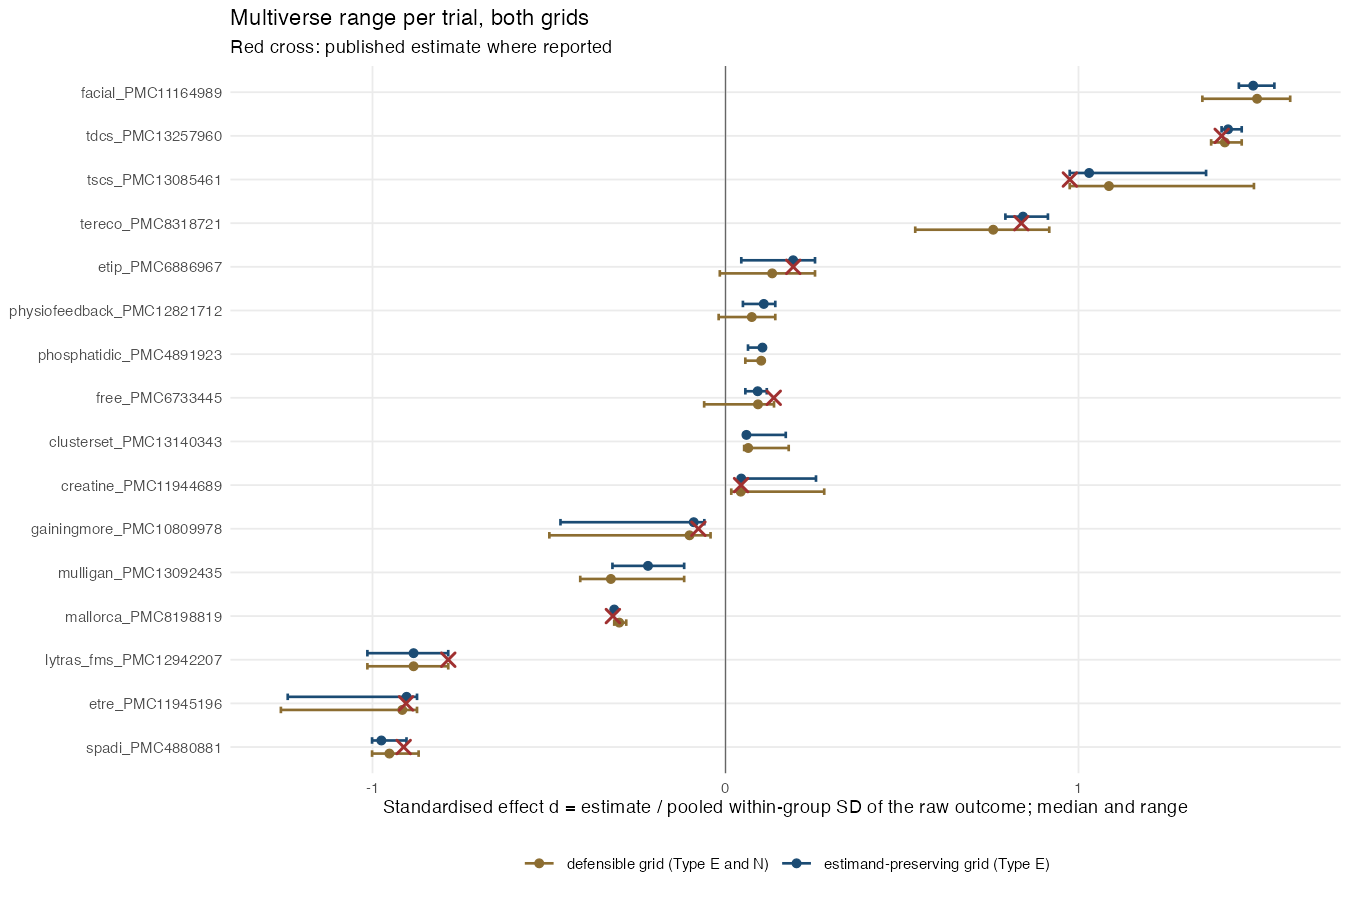
\includegraphics[width=\textwidth,height=0.85\textheight,keepaspectratio]{figures/supp/overview_all_studies.png}}

\section{Figure S2. Share of interval-width variance per node}\label{figure-s2.-share-of-interval-width-variance-per-node}

\pandocbounded{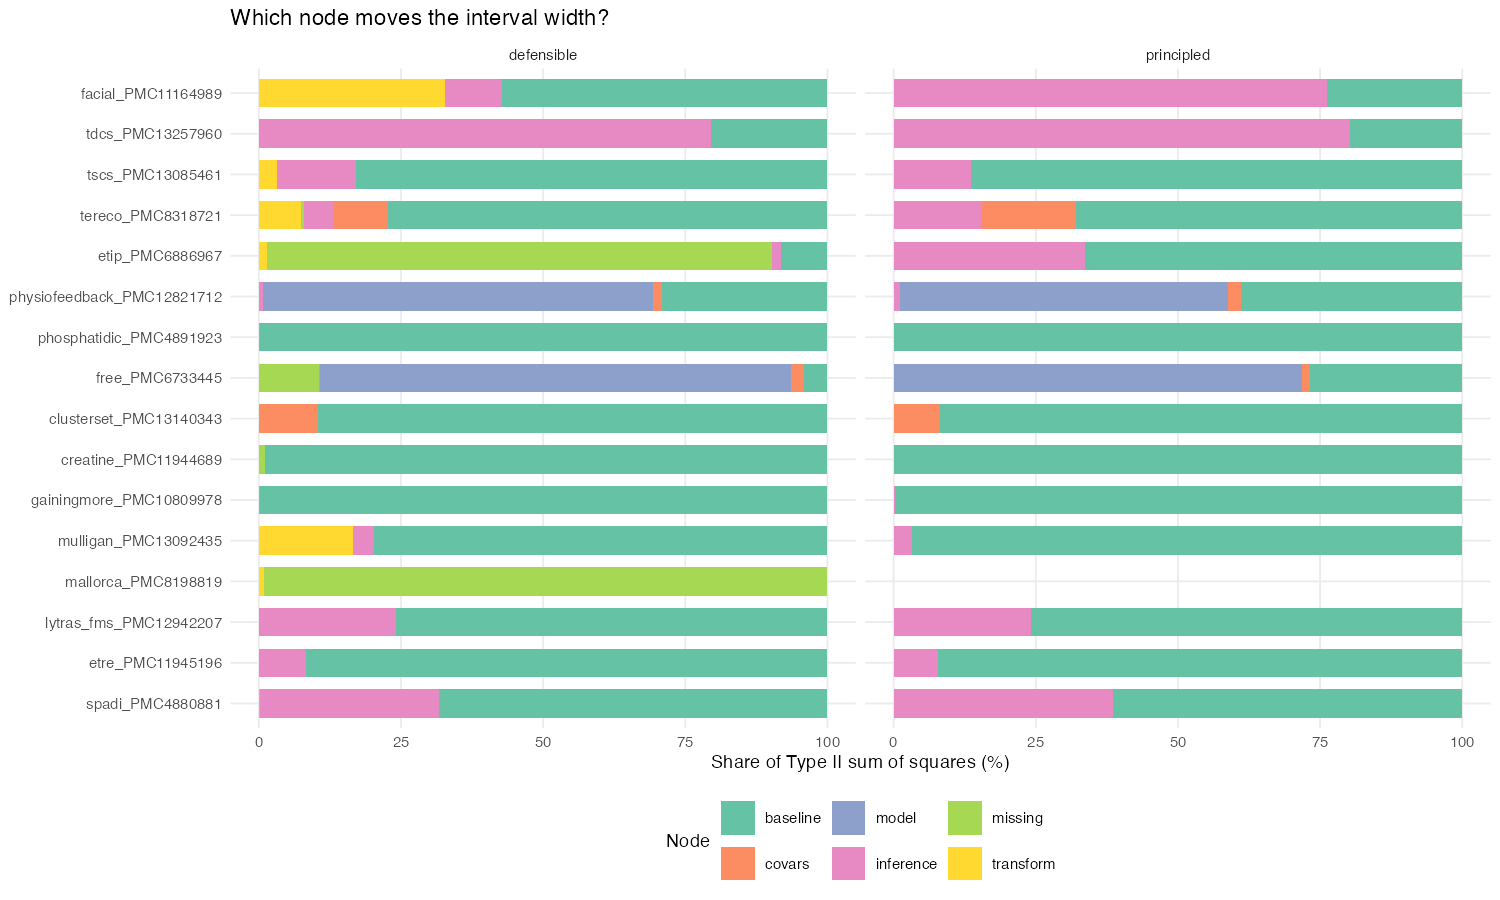
\includegraphics[width=\textwidth,height=0.85\textheight,keepaspectratio]{figures/supp/variance_ci_width_d.png}}

\section{Figure S3. Specification curves, clusterset\_PMC13140343}\label{figure-s3.-specification-curves-clusterset_pmc13140343}

\pandocbounded{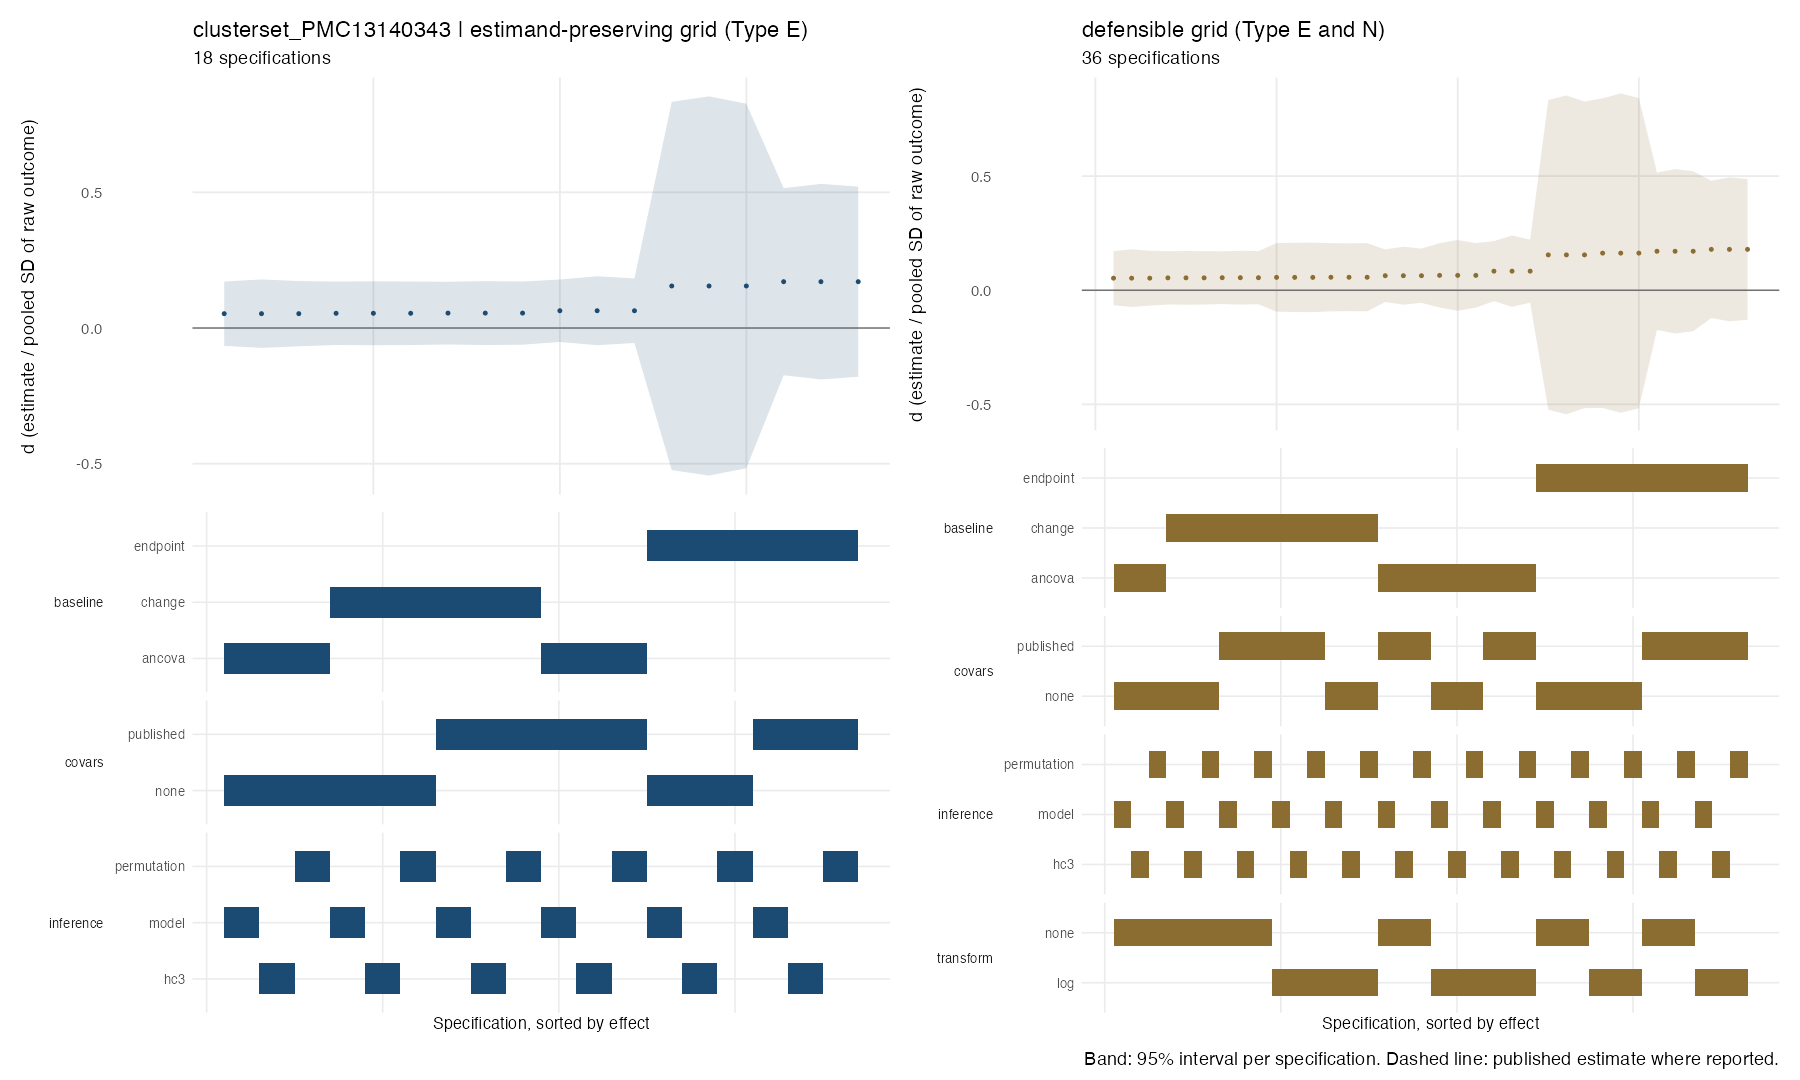
\includegraphics[width=\textwidth,height=0.85\textheight,keepaspectratio]{figures/supp/speccurve_clusterset_PMC13140343.png}}

\section{Figure S4. Specification curves, creatine\_PMC11944689}\label{figure-s4.-specification-curves-creatine_pmc11944689}

\pandocbounded{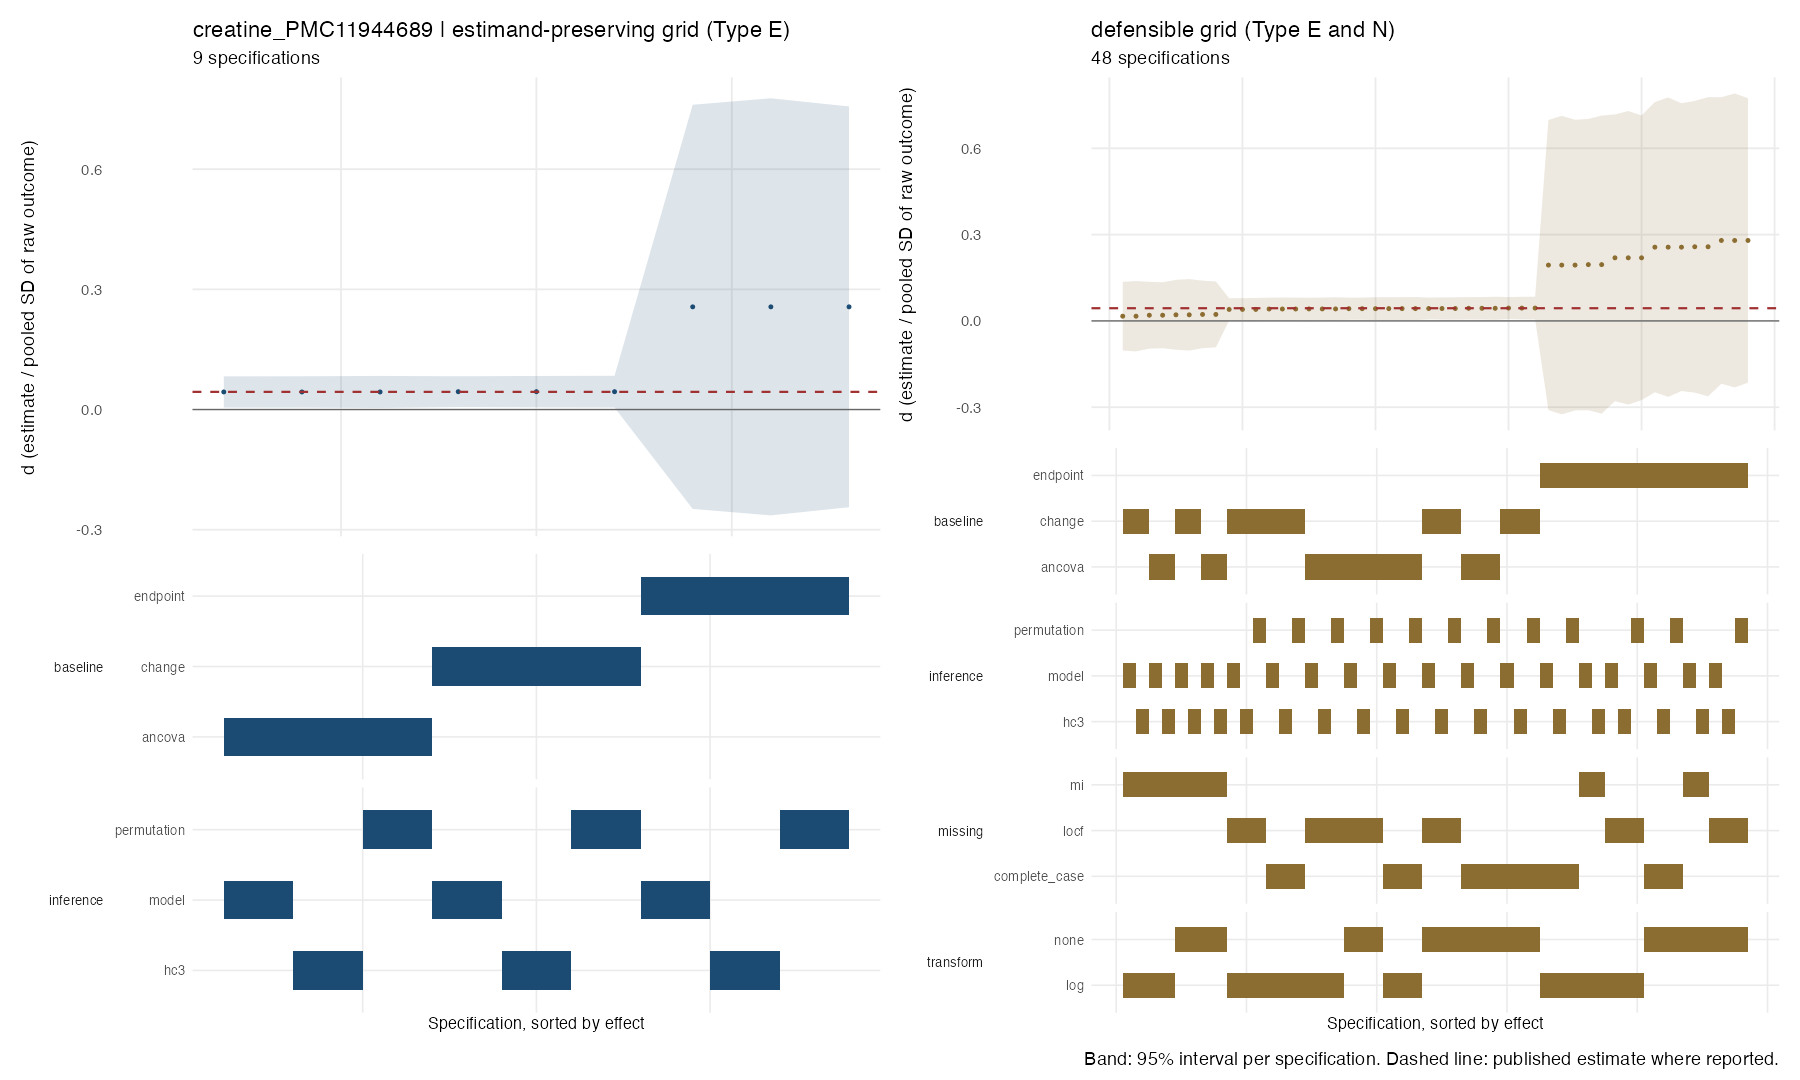
\includegraphics[width=\textwidth,height=0.85\textheight,keepaspectratio]{figures/supp/speccurve_creatine_PMC11944689.png}}

\section{Figure S5. Specification curves, etip\_PMC6886967}\label{figure-s5.-specification-curves-etip_pmc6886967}

\pandocbounded{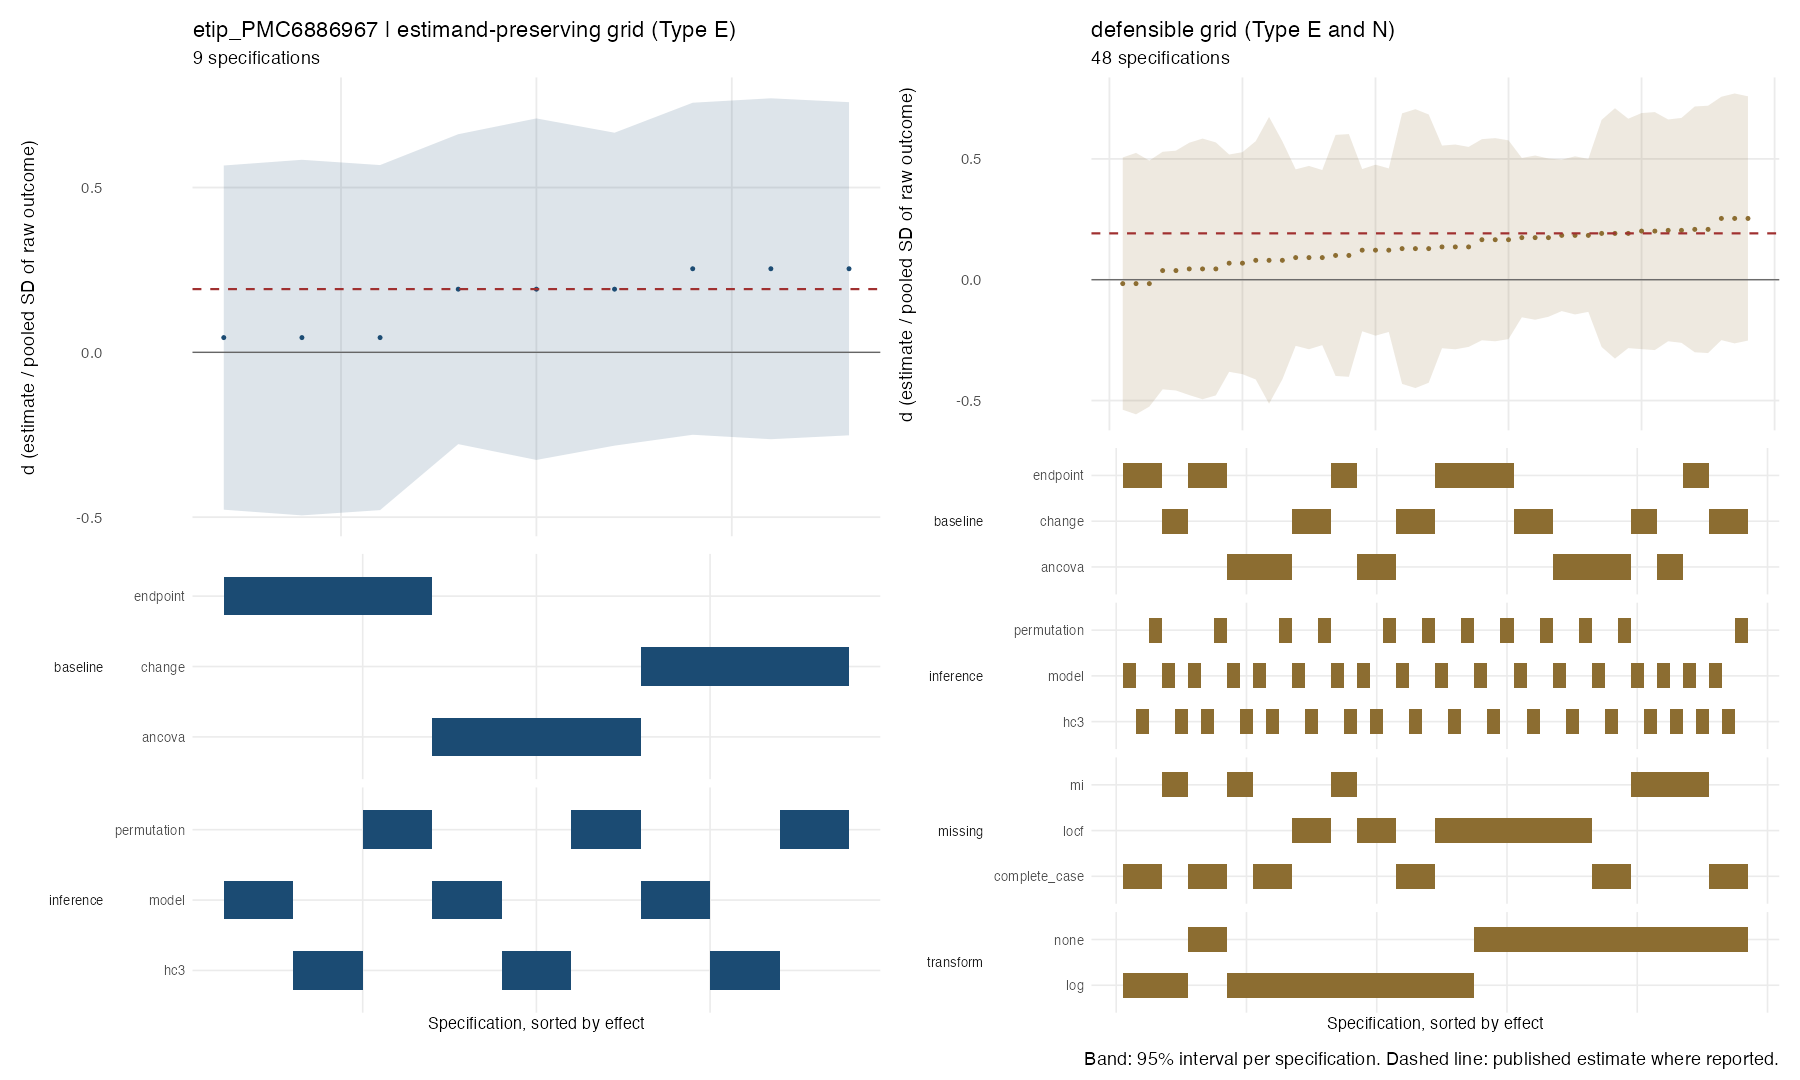
\includegraphics[width=\textwidth,height=0.85\textheight,keepaspectratio]{figures/supp/speccurve_etip_PMC6886967.png}}

\section{Figure S6. Specification curves, etre\_PMC11945196}\label{figure-s6.-specification-curves-etre_pmc11945196}

\pandocbounded{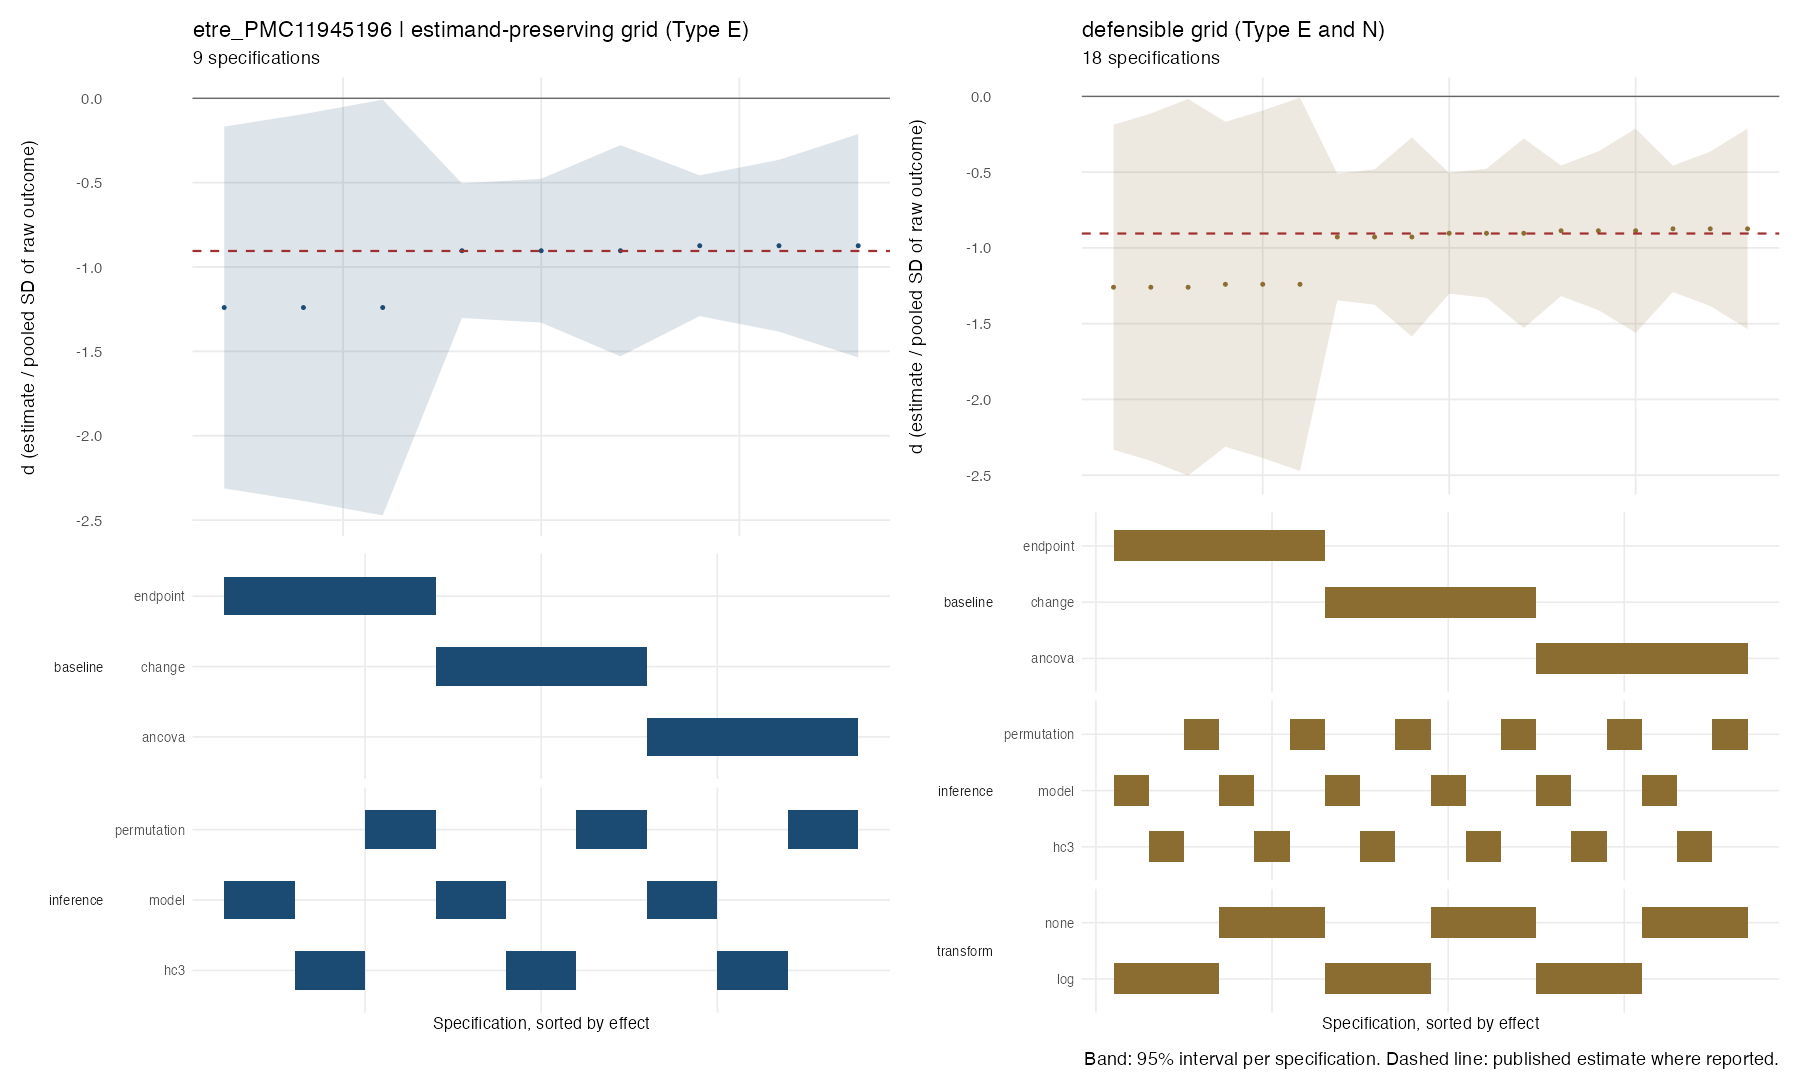
\includegraphics[width=\textwidth,height=0.85\textheight,keepaspectratio]{figures/supp/speccurve_etre_PMC11945196.png}}

\section{Figure S7. Specification curves, facial\_PMC11164989}\label{figure-s7.-specification-curves-facial_pmc11164989}

\pandocbounded{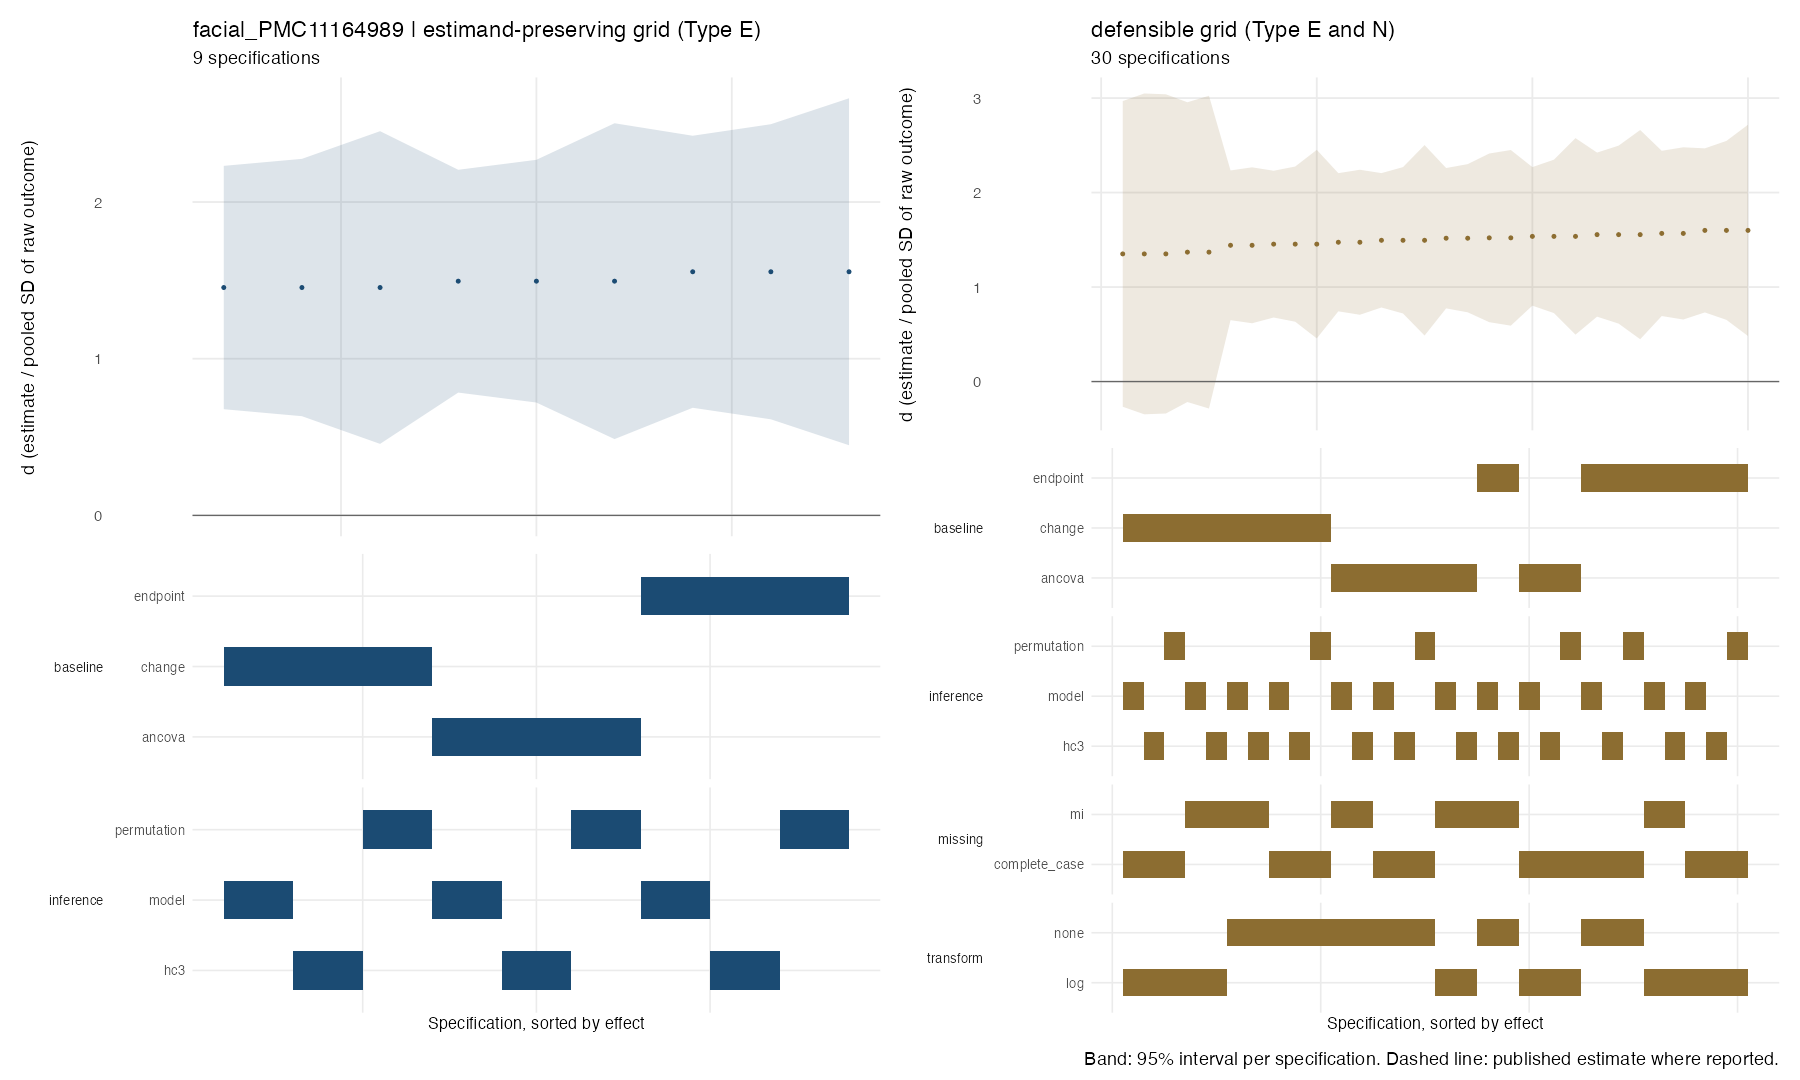
\includegraphics[width=\textwidth,height=0.85\textheight,keepaspectratio]{figures/supp/speccurve_facial_PMC11164989.png}}

\section{Figure S8. Specification curves, free\_PMC6733445}\label{figure-s8.-specification-curves-free_pmc6733445}

\pandocbounded{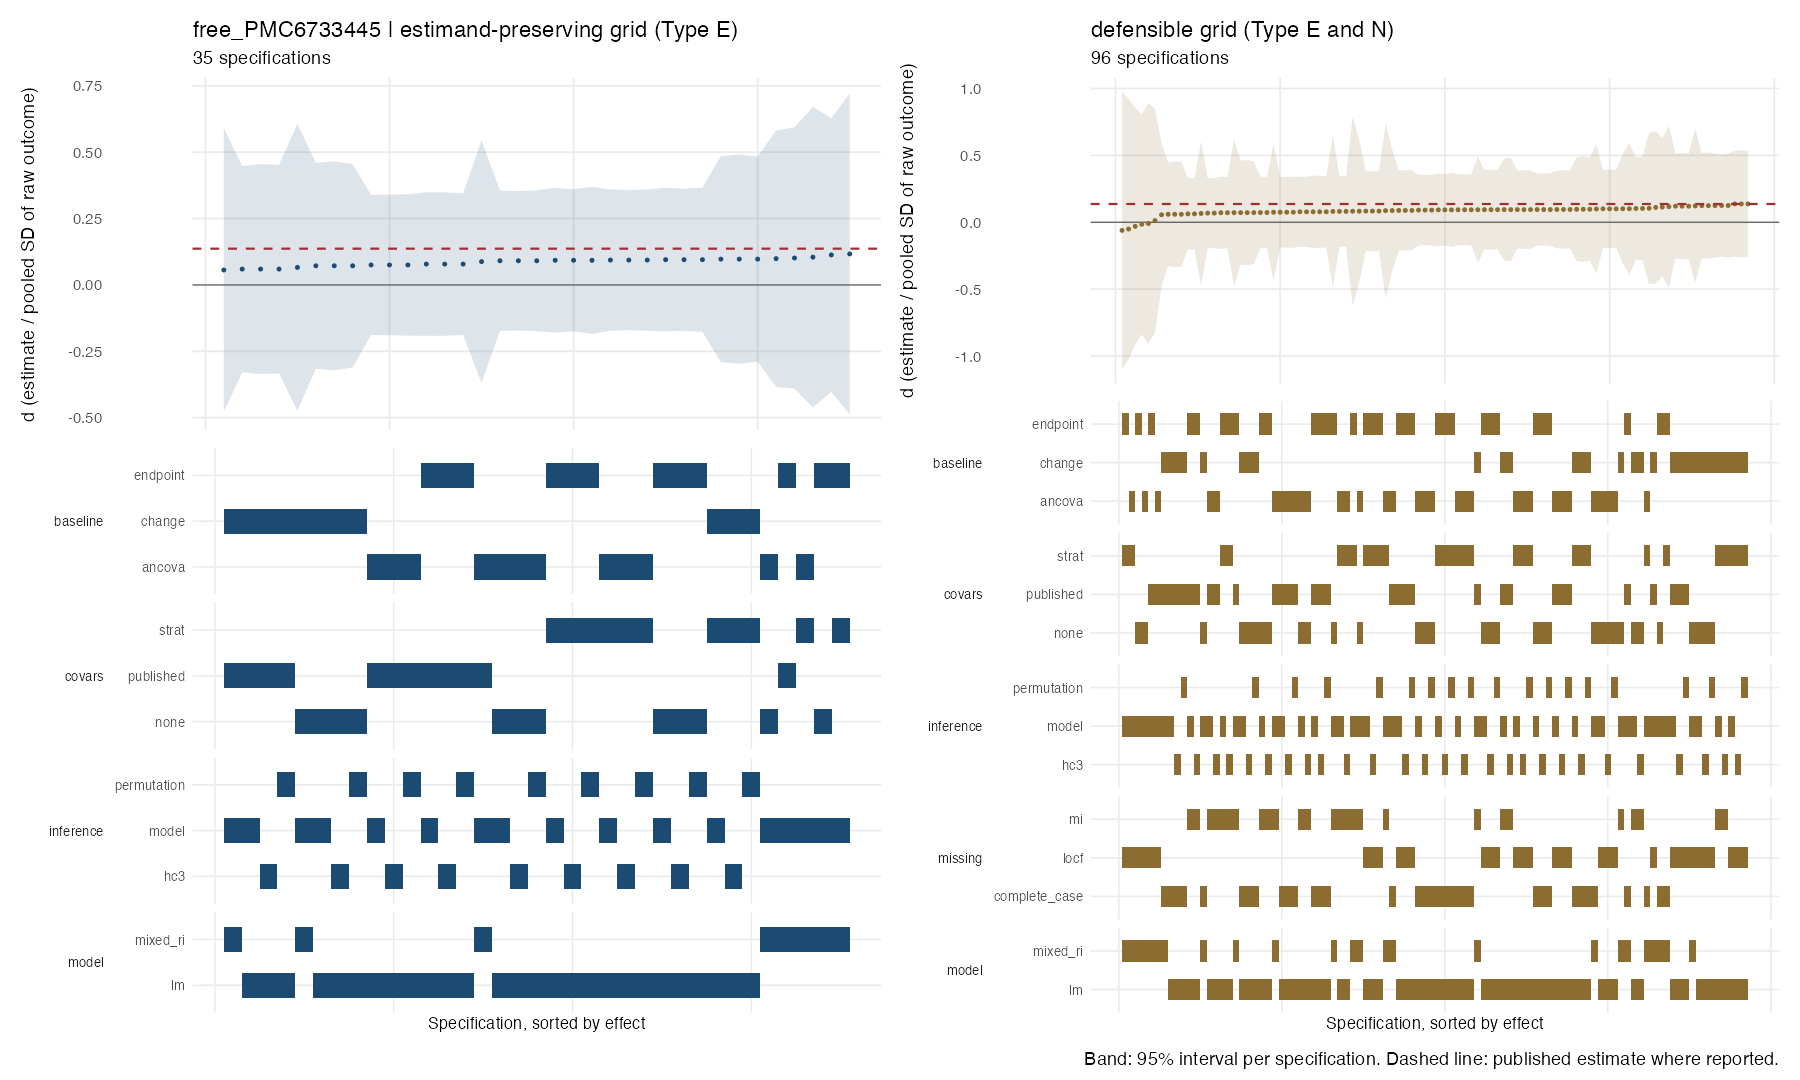
\includegraphics[width=\textwidth,height=0.85\textheight,keepaspectratio]{figures/supp/speccurve_free_PMC6733445.png}}

\section{Figure S9. Specification curves, gainingmore\_PMC10809978}\label{figure-s9.-specification-curves-gainingmore_pmc10809978}

\pandocbounded{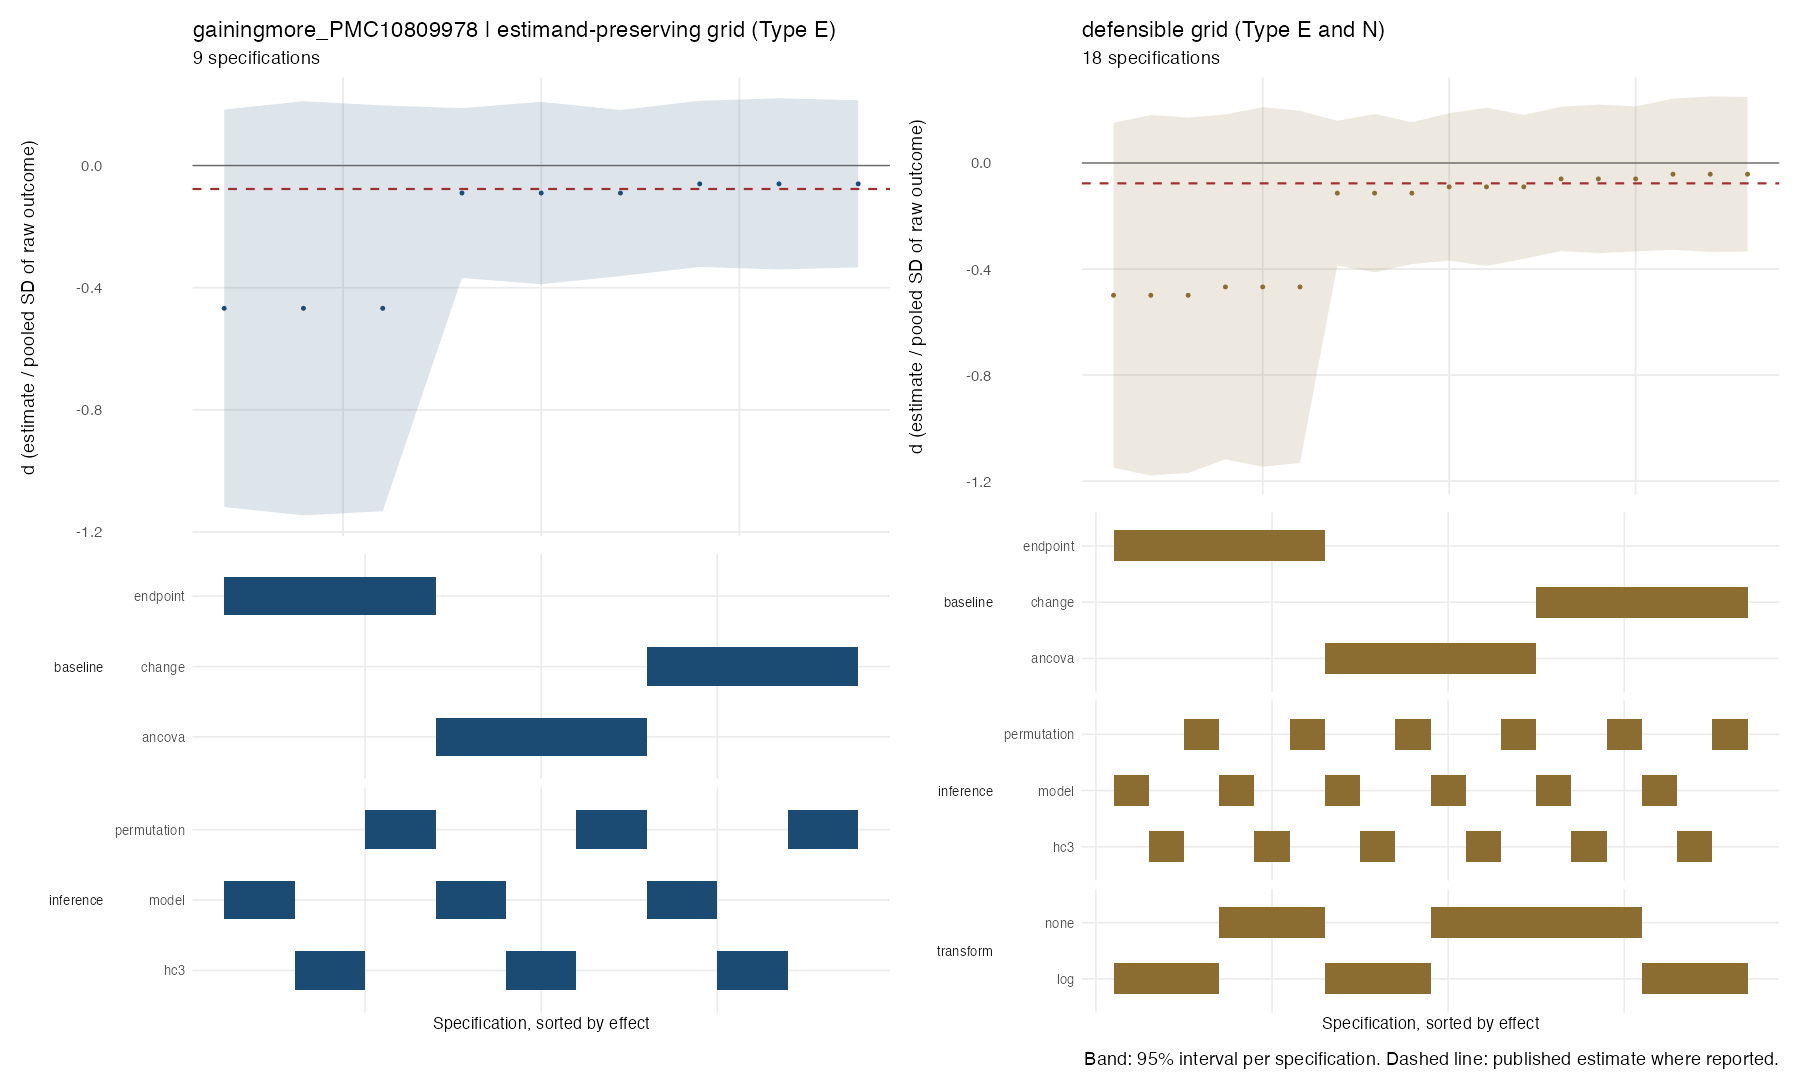
\includegraphics[width=\textwidth,height=0.85\textheight,keepaspectratio]{figures/supp/speccurve_gainingmore_PMC10809978.png}}

\section{Figure S10. Specification curves, lytras\_fms\_PMC12942207}\label{figure-s10.-specification-curves-lytras_fms_pmc12942207}

\pandocbounded{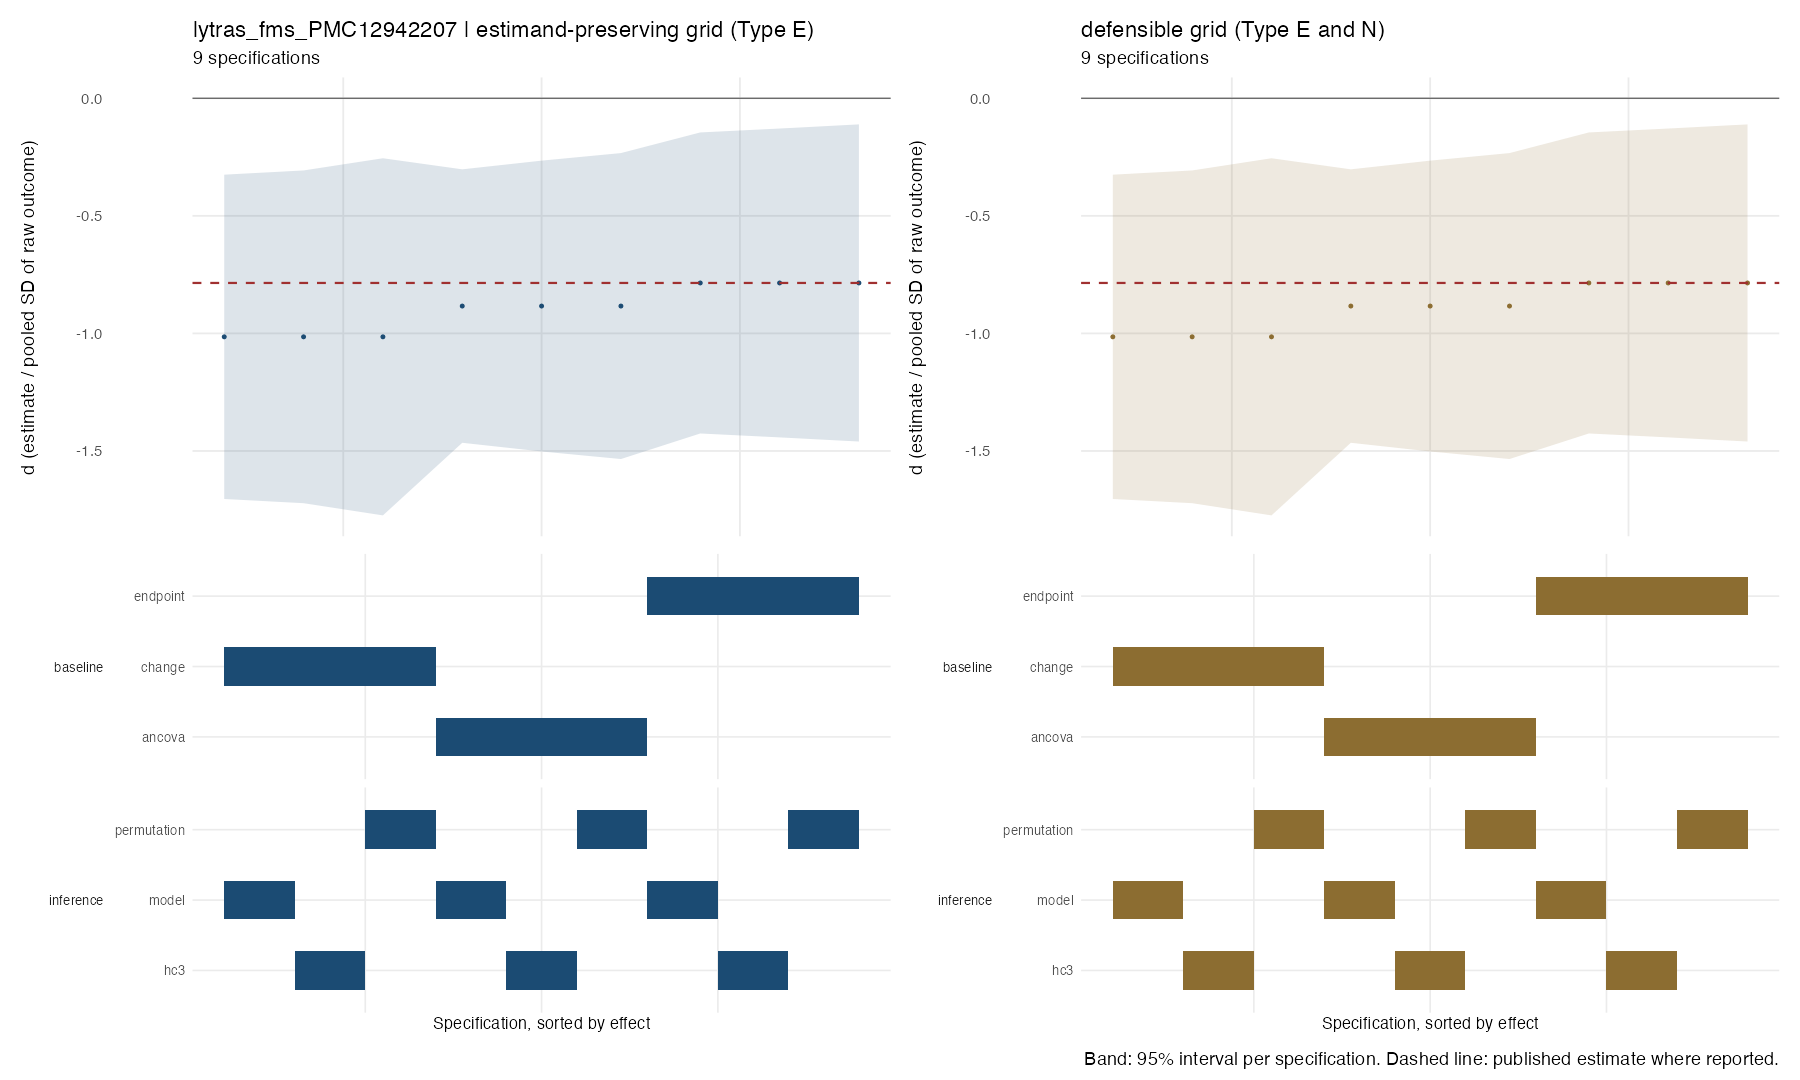
\includegraphics[width=\textwidth,height=0.85\textheight,keepaspectratio]{figures/supp/speccurve_lytras_fms_PMC12942207.png}}

\section{Figure S11. Specification curves, mallorca\_PMC8198819}\label{figure-s11.-specification-curves-mallorca_pmc8198819}

\pandocbounded{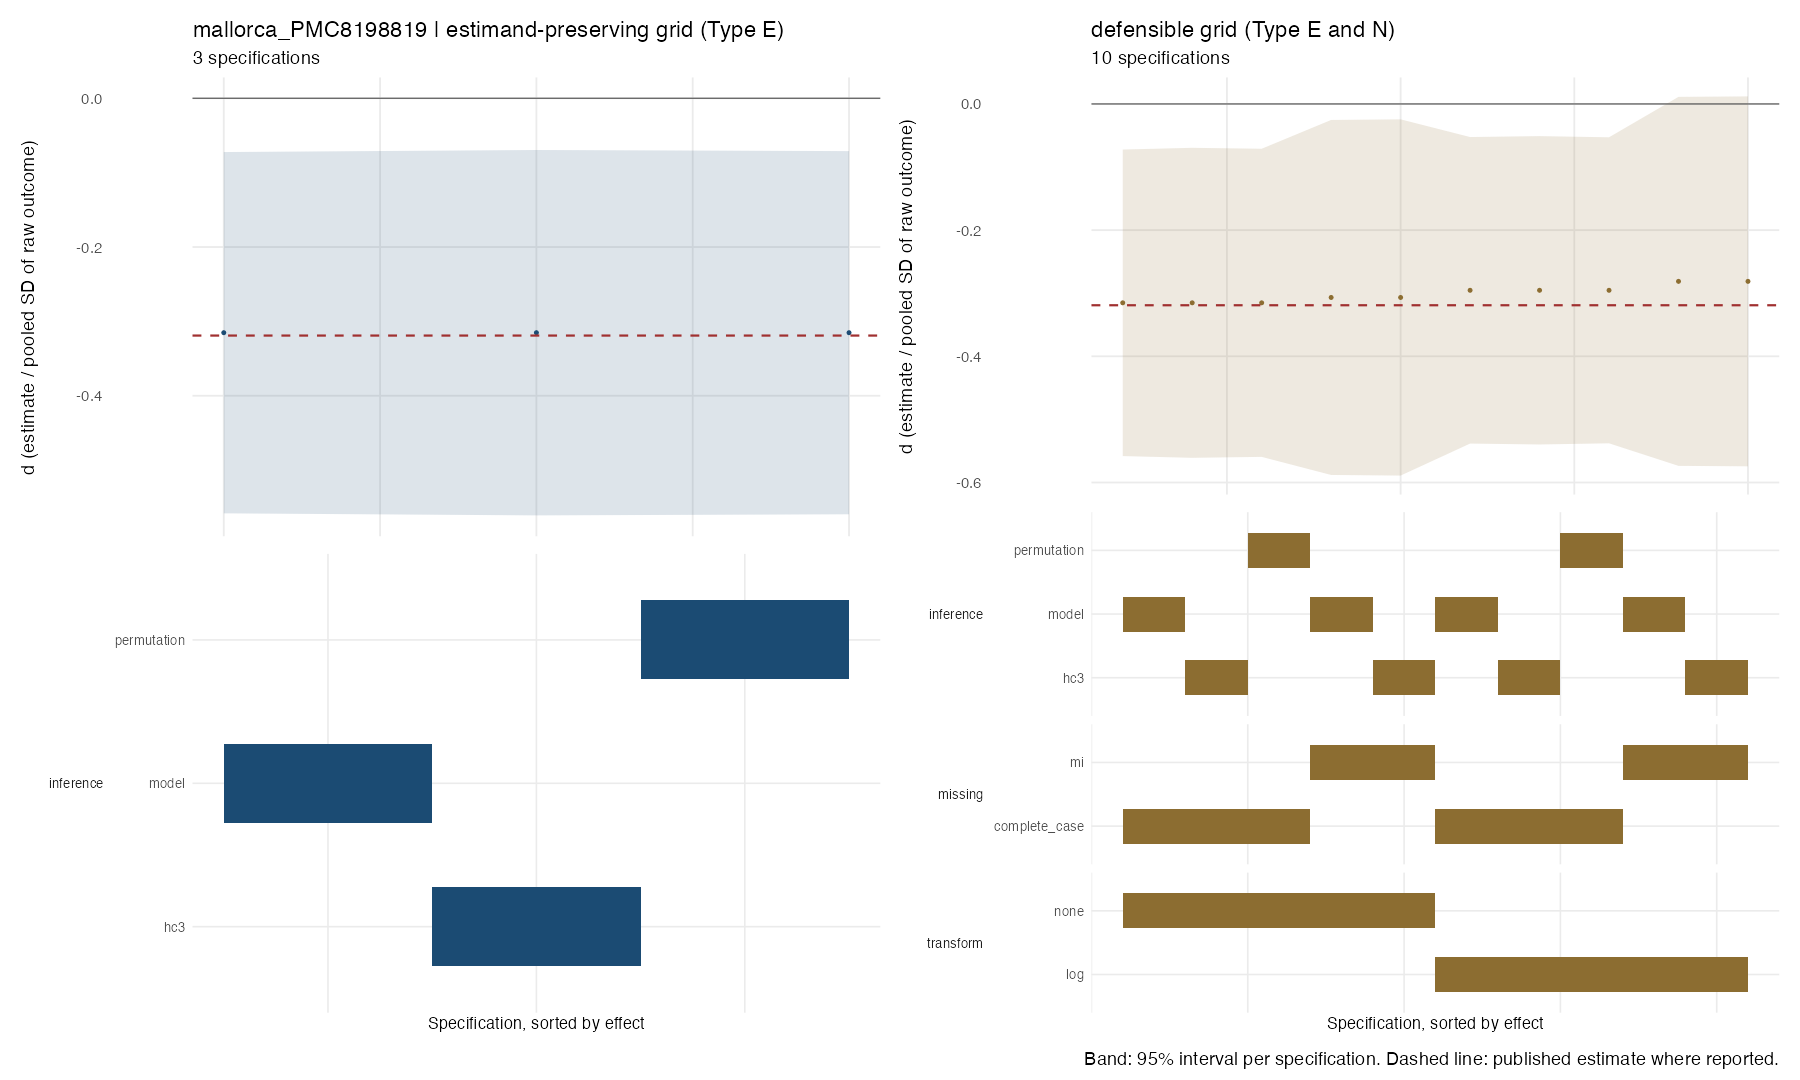
\includegraphics[width=\textwidth,height=0.85\textheight,keepaspectratio]{figures/supp/speccurve_mallorca_PMC8198819.png}}

\section{Figure S12. Specification curves, mulligan\_PMC13092435}\label{figure-s12.-specification-curves-mulligan_pmc13092435}

\pandocbounded{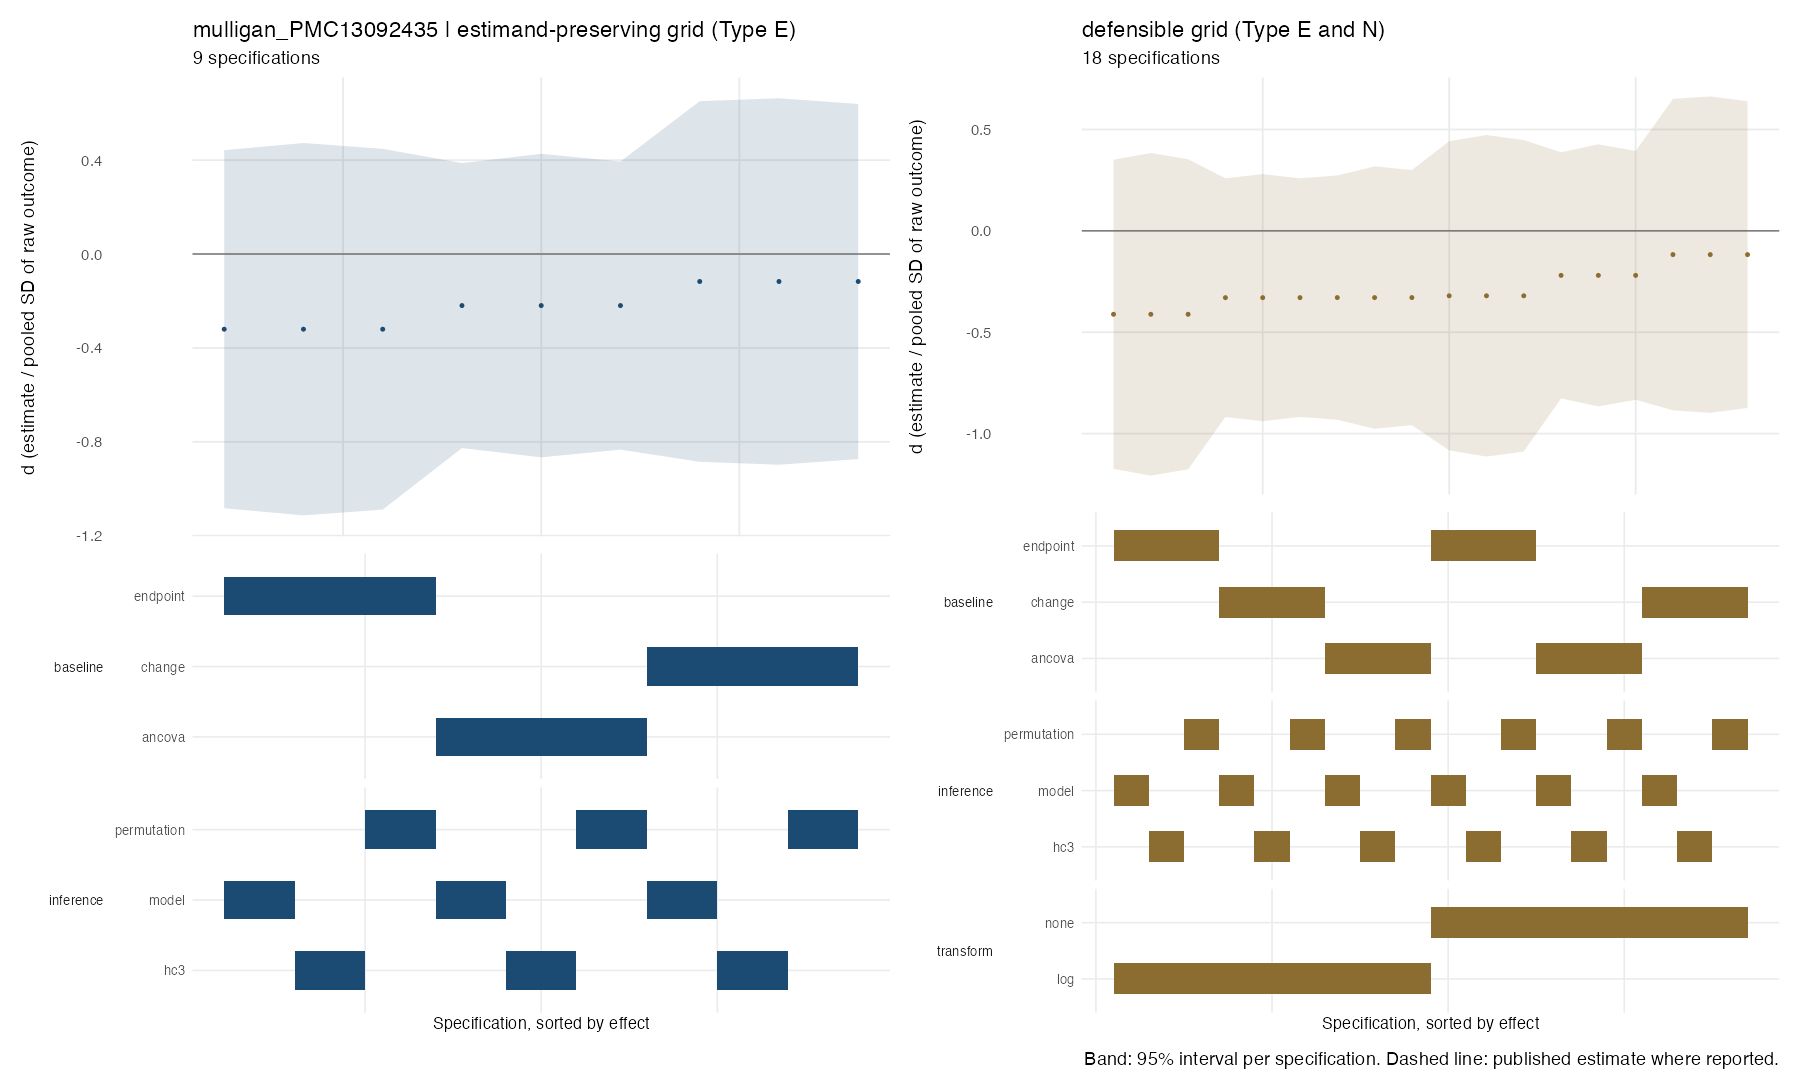
\includegraphics[width=\textwidth,height=0.85\textheight,keepaspectratio]{figures/supp/speccurve_mulligan_PMC13092435.png}}

\section{Figure S13. Specification curves, phosphatidic\_PMC4891923}\label{figure-s13.-specification-curves-phosphatidic_pmc4891923}

\pandocbounded{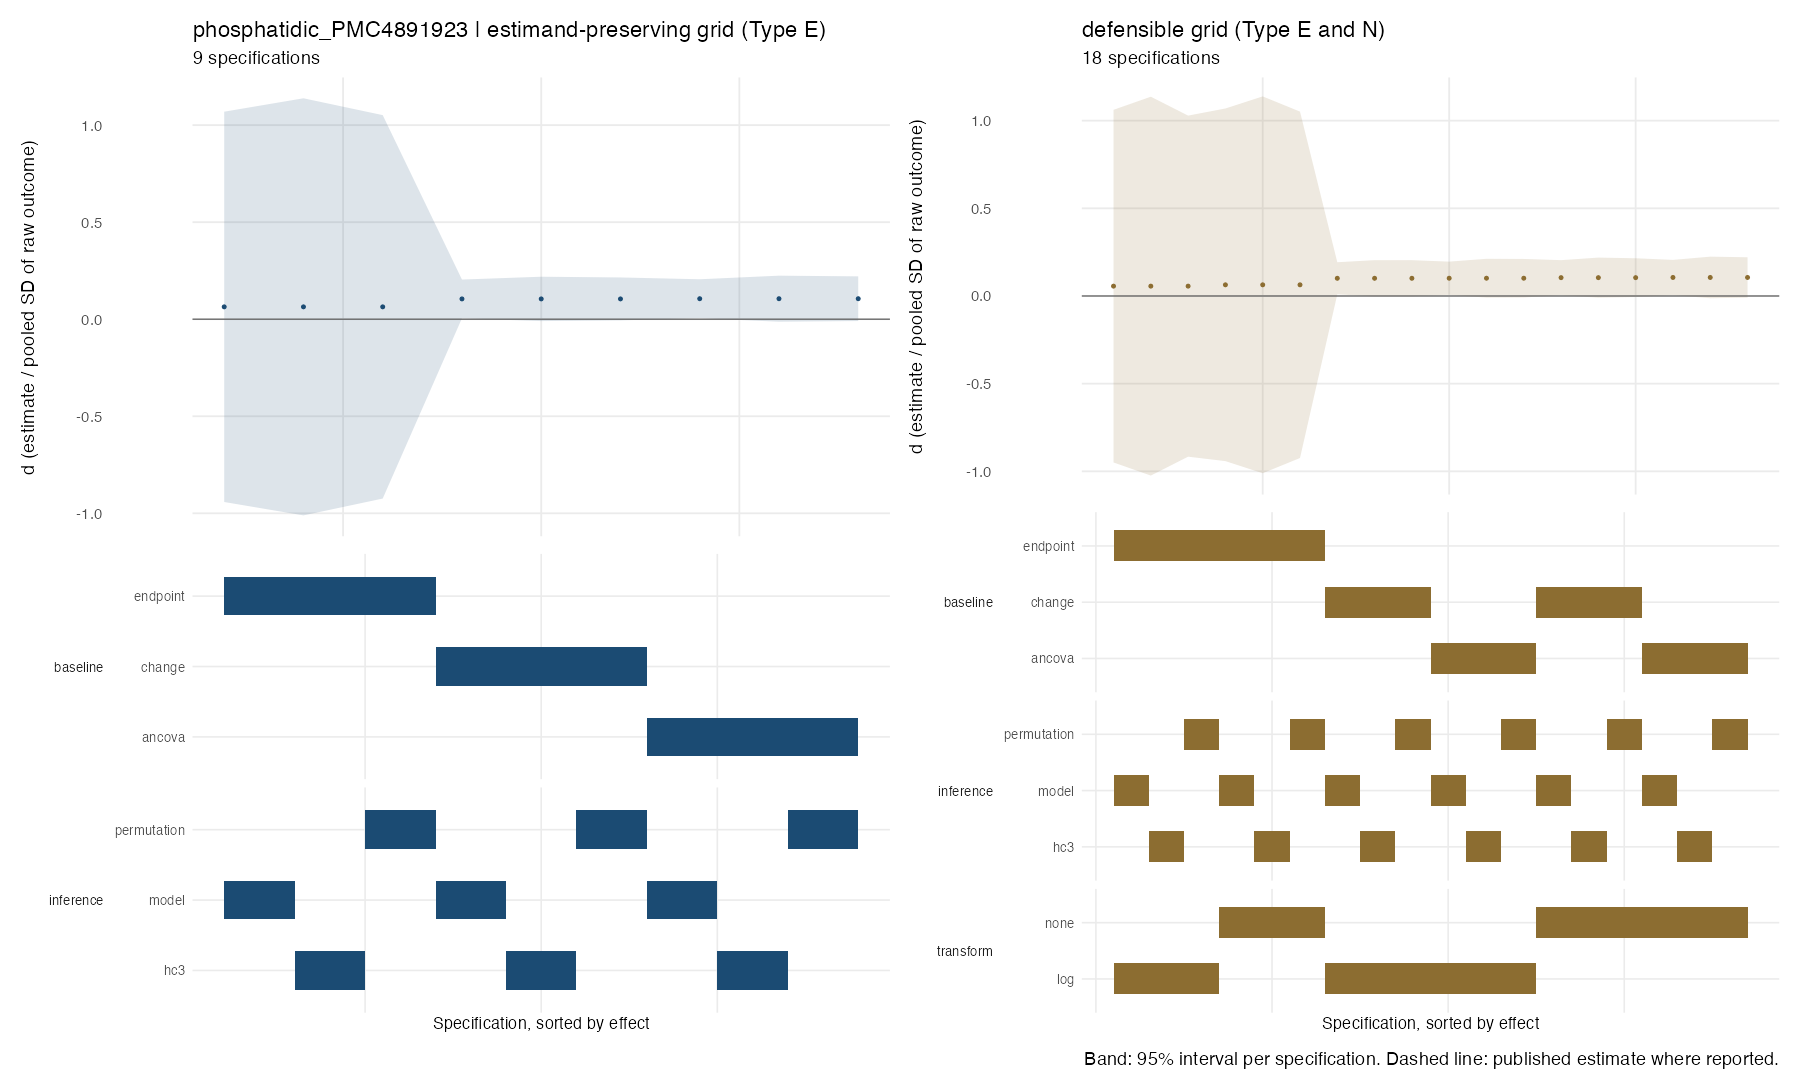
\includegraphics[width=\textwidth,height=0.85\textheight,keepaspectratio]{figures/supp/speccurve_phosphatidic_PMC4891923.png}}

\section{Figure S14. Specification curves, physiofeedback\_PMC12821712}\label{figure-s14.-specification-curves-physiofeedback_pmc12821712}

\pandocbounded{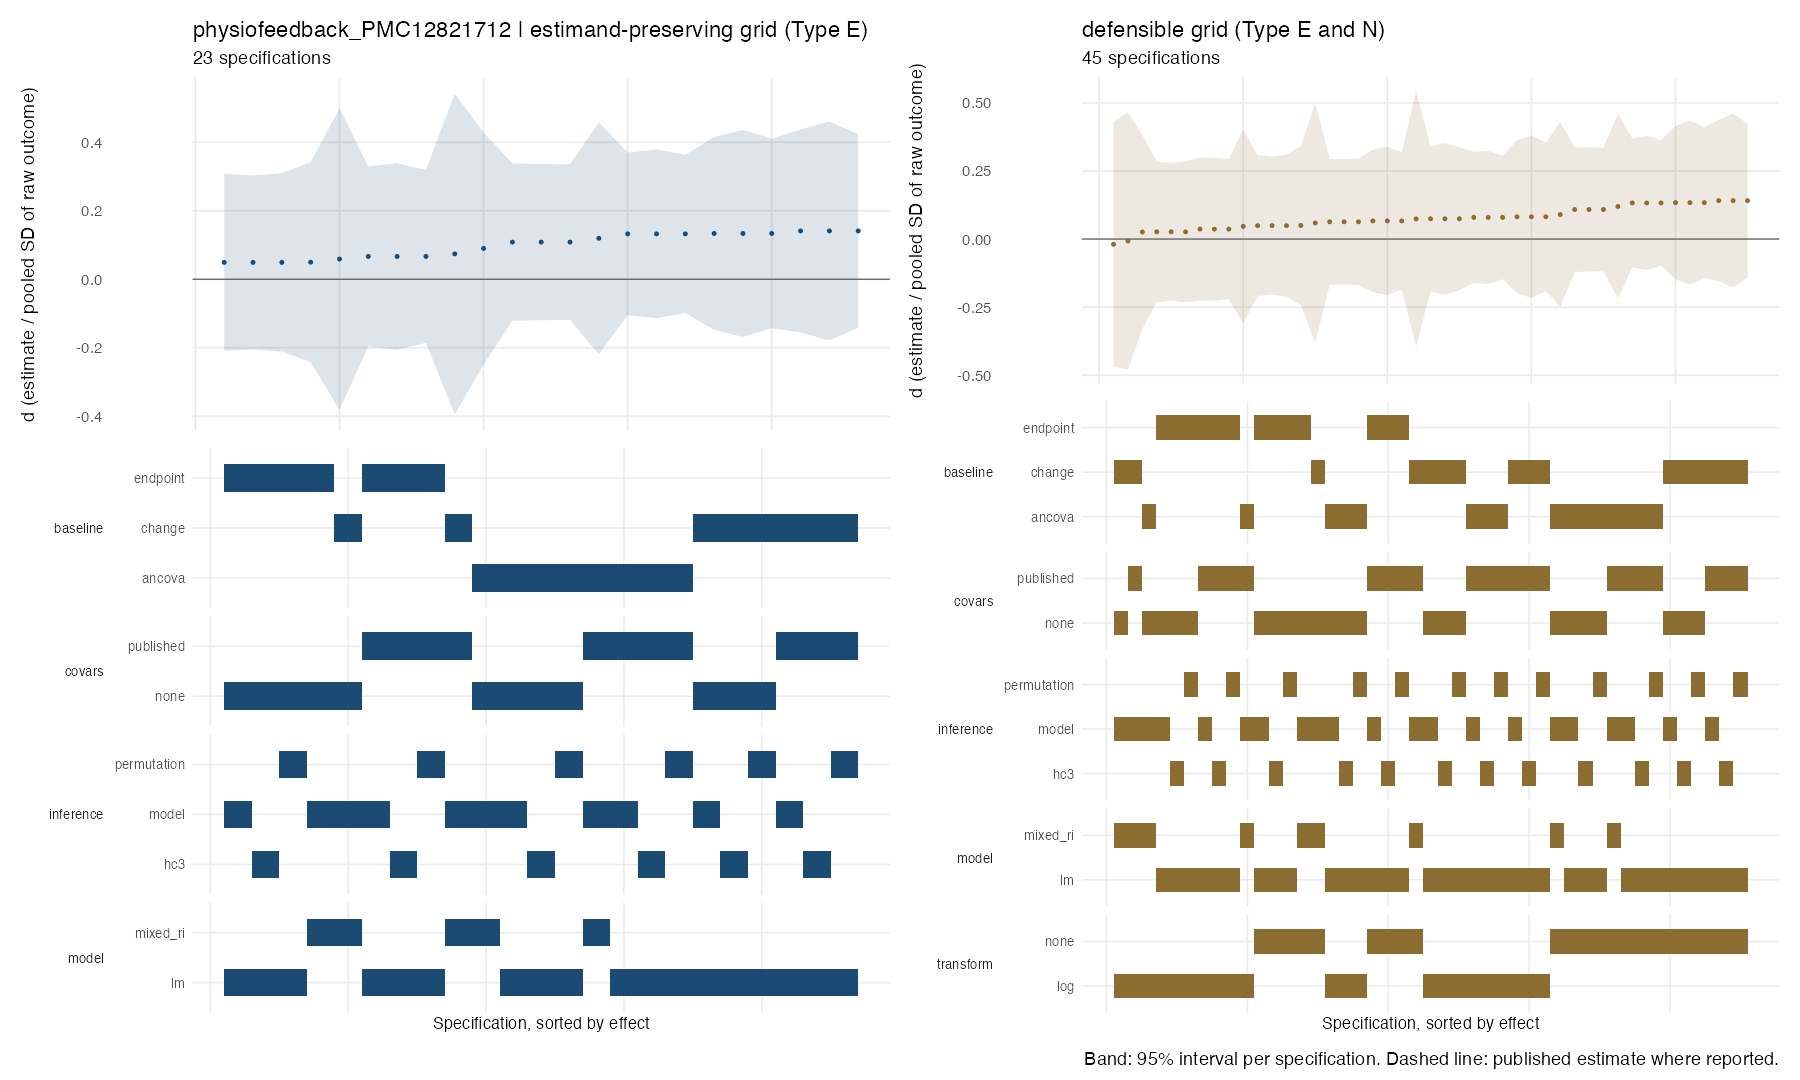
\includegraphics[width=\textwidth,height=0.85\textheight,keepaspectratio]{figures/supp/speccurve_physiofeedback_PMC12821712.png}}

\section{Figure S15. Specification curves, spadi\_PMC4880881}\label{figure-s15.-specification-curves-spadi_pmc4880881}

\pandocbounded{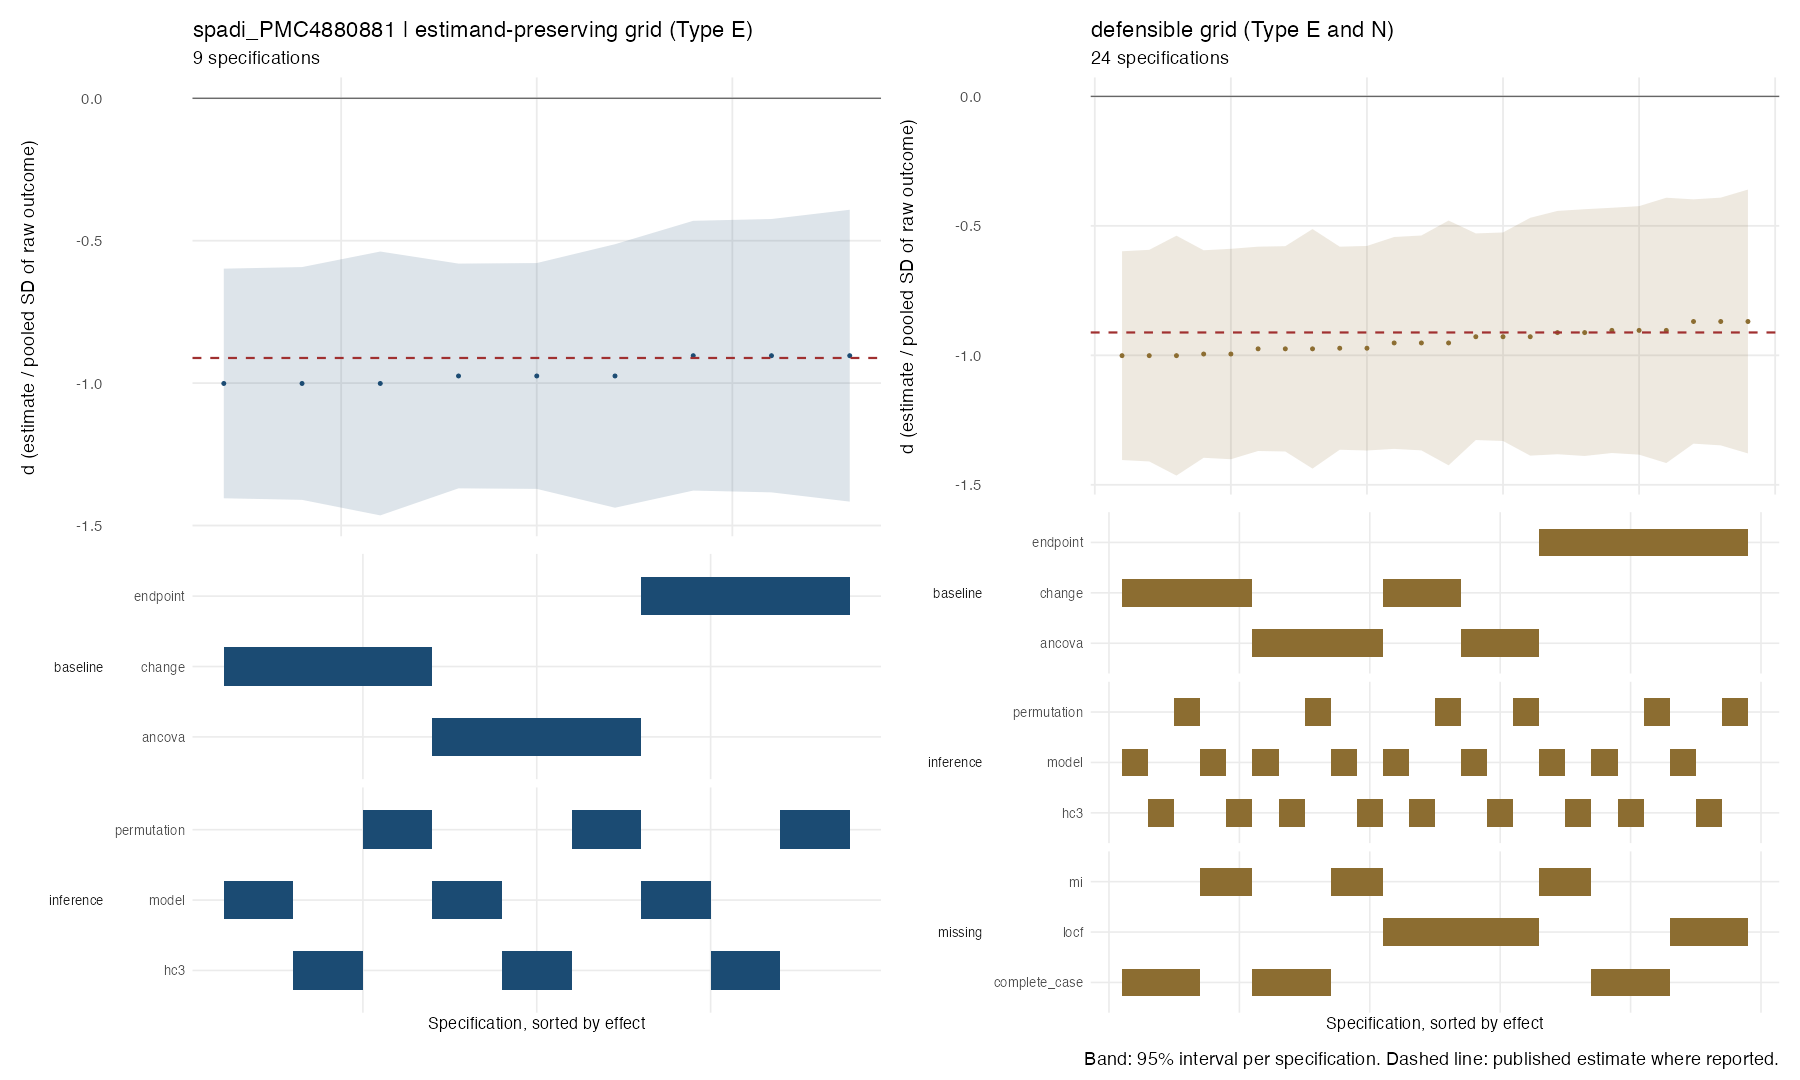
\includegraphics[width=\textwidth,height=0.85\textheight,keepaspectratio]{figures/supp/speccurve_spadi_PMC4880881.png}}

\section{Figure S16. Specification curves, tdcs\_PMC13257960}\label{figure-s16.-specification-curves-tdcs_pmc13257960}

\pandocbounded{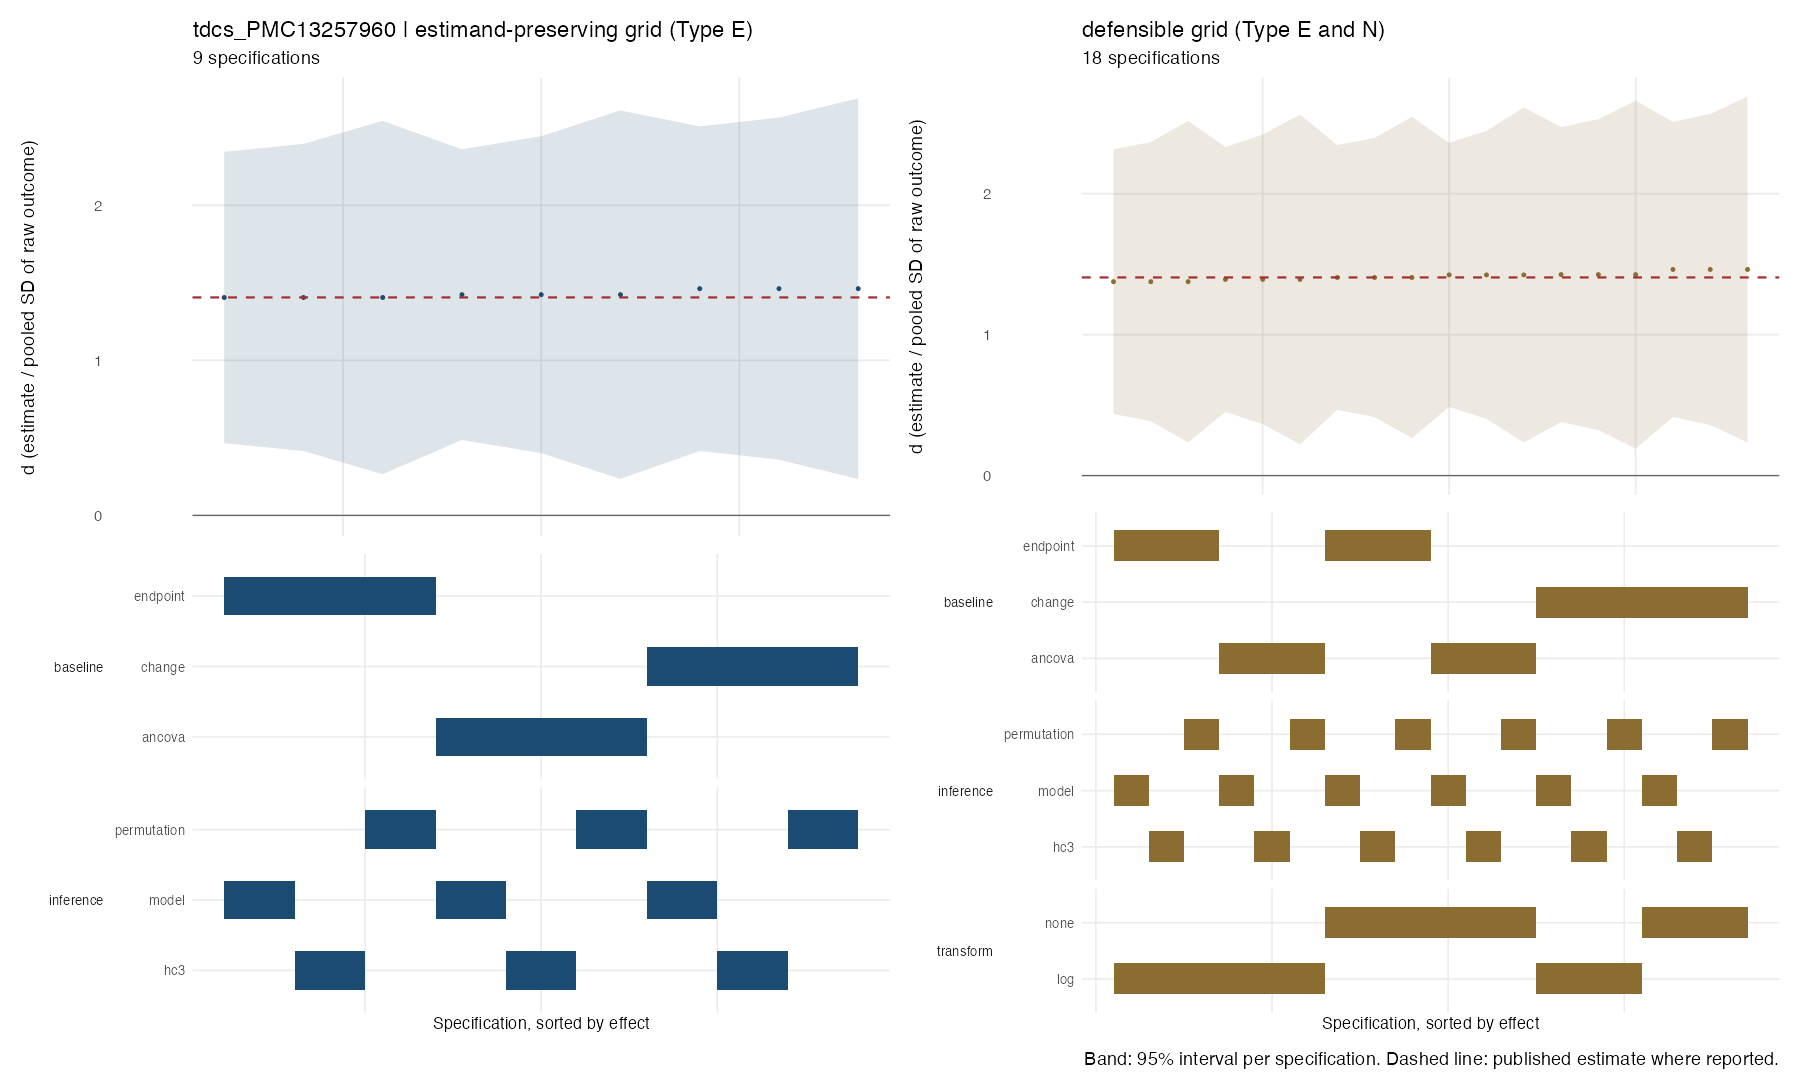
\includegraphics[width=\textwidth,height=0.85\textheight,keepaspectratio]{figures/supp/speccurve_tdcs_PMC13257960.png}}

\section{Figure S17. Specification curves, tereco\_PMC8318721}\label{figure-s17.-specification-curves-tereco_pmc8318721}

\pandocbounded{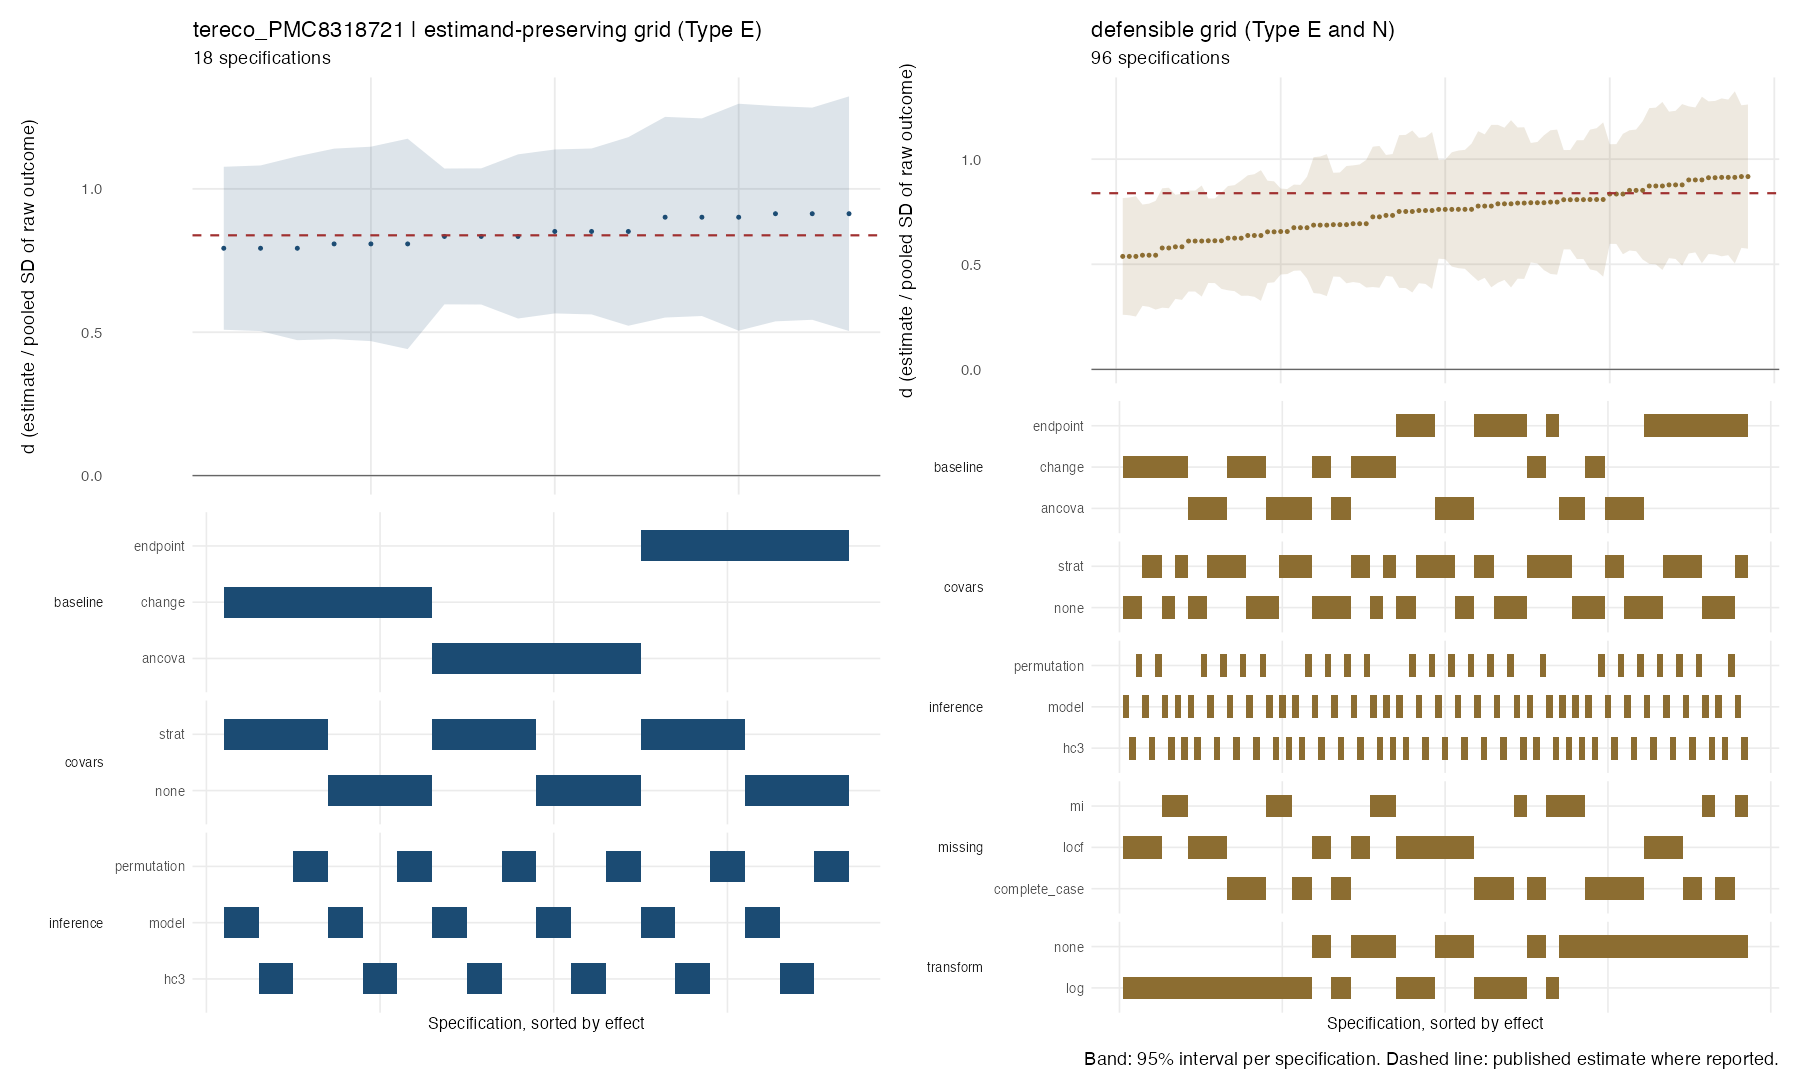
\includegraphics[width=\textwidth,height=0.85\textheight,keepaspectratio]{figures/supp/speccurve_tereco_PMC8318721.png}}

\section{Figure S18. Specification curves, tscs\_PMC13085461}\label{figure-s18.-specification-curves-tscs_pmc13085461}

\pandocbounded{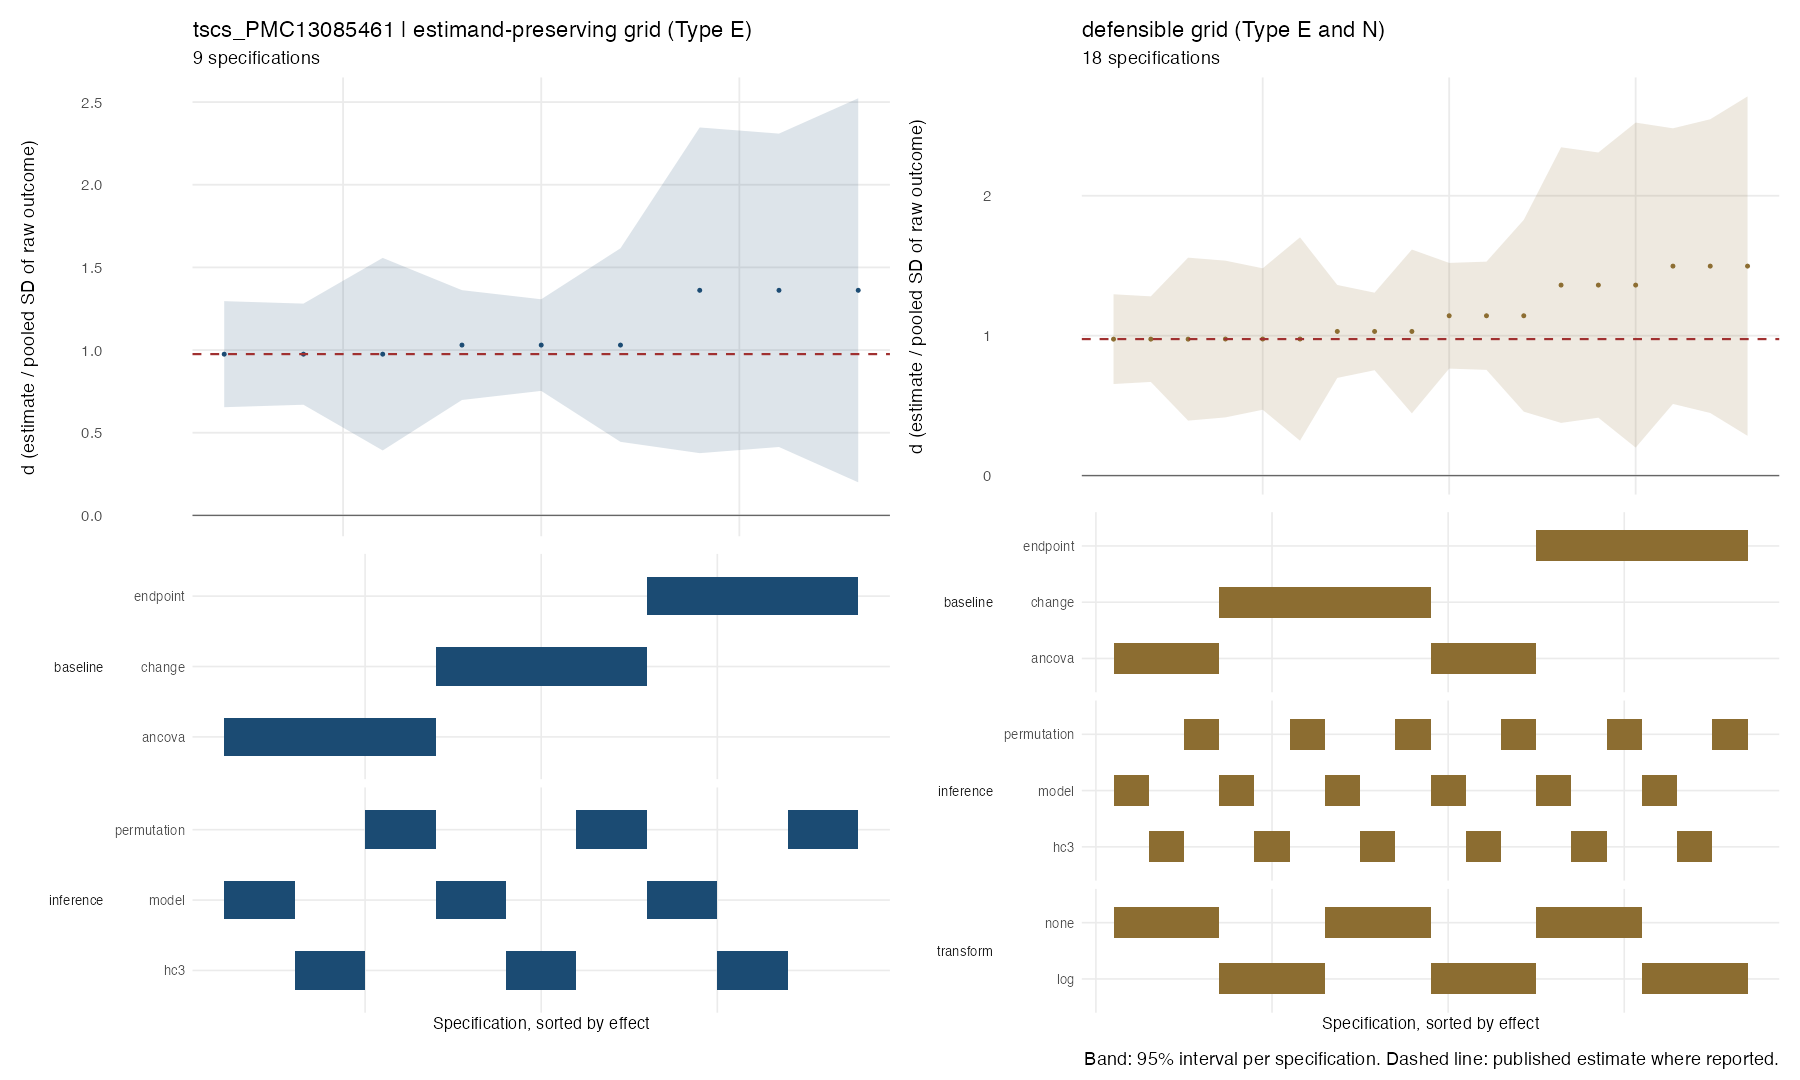
\includegraphics[width=\textwidth,height=0.85\textheight,keepaspectratio]{figures/supp/speccurve_tscs_PMC13085461.png}}

\section{Text S2. Novelty search protocol, 15 September 2026}\label{text-s2.-novelty-search-protocol-15-september-2026}

\subsection{Neuheitsprüfung, 2026-09-15}\label{neuheitspruxfcfung-2026-09-15}

Geprüfte Aussage (Manuskript, \texttt{body.tex} Zeile 5 bzw. \texttt{paper.md}):

\begin{quote}
``I am not aware of a study in physiotherapy, rehabilitation or exercise science that retrieved individual participant data from public repositories and recomputed the published primary analysis.''
\end{quote}

Kriterium für ein Gegenbeispiel: Individualdaten aus einem öffentlichen Repositorium oder Supplement geholt \textbf{UND} die publizierte Primäranalyse nachgerechnet, im Feld Physiotherapie, Rehabilitation oder Sport- und Bewegungswissenschaft.

Diese Prüfung ergänzt die frühere Neuheitsprüfung vom 2026-08-28 (dokumentiert in \texttt{README.md}, Abschnitt ``Neuheitsprüfung''). Die dort ausgeschlossenen Nachbarn (Jabouille 2025, Elghzali 2025, Murphy 2025, Dhanani 2022) werden hier nicht erneut im Volltext geprüft, sondern als bekannt vorausgesetzt.

\textbf{Urteil vorab: Kein Gegenbeispiel gefunden. Die Aussage bleibt haltbar.} Der nächste Nachbar ist eine seit Januar 2026 laufende, noch nicht abgeschlossene Registered-Report- Studie aus der Sportwissenschaft, die die publizierte Primäranalyse zwar nachrechnen will, aber ausdrücklich mit \textbf{privaten}, von Autoren vertraulich geteilten Rohdaten arbeitet statt mit Daten aus einem öffentlichen Repositorium. Details unten.

\subsection{Methodik und Abweichungen vom Suchplan}\label{methodik-und-abweichungen-vom-suchplan}

Alle Anfragen liefen über curl mit \texttt{-A\ "Mozilla/5.0"} und 1,5 Sekunden Pause zwischen Aufrufen. Zwei Abweichungen von der Suchvorgabe, beide dokumentiert:

\begin{enumerate}
\def\labelenumi{\arabic{enumi}.}
\tightlist
\item
  \textbf{medRxiv/bioRxiv}: Die direkte HTML-Suche auf \texttt{www.medrxiv.org/search/...} liefert nur eine Cloudflare-Challenge-Seite (``Just a moment\ldots{}'') zurück, kein Suchergebnis. Wie im Suchplan selbst vorgesehen, wurde stattdessen OpenAlex mit \texttt{filter=type:preprint} verwendet.
\item
  \textbf{OSF Registrations}: \texttt{https://api.osf.io/v2/registrations/} lieferte während der gesamten Sitzung durchgehend HTTP 502 oder Verbindungs-Timeouts (\texttt{https://api.osf.io/v2/} selbst antwortete mit 200, nur der Registrations-Endpunkt war betroffen; mehrere Wiederholungen über rund zwei Minuten, kein Erfolg). Als Ersatz wurde die SHARE-Such-API (\texttt{https://share.osf.io/api/v2/search/creativeworks/\_search}) verwendet, die auch OSF-Registrierungen indiziert und zum Suchzeitpunkt erreichbar war (HTTP 200). Das ist ein dokumentierter Kompromiss, kein vollständiger Ersatz für \texttt{filter{[}title{]}}, weil SHARE eine andere Relevanzgewichtung nutzt und weitere Quellen (CrossRef, DataCite, PubMed Central) mit indiziert.
\end{enumerate}

\subsection{Abfragen wörtlich, mit Quelle und Trefferzahl}\label{abfragen-wuxf6rtlich-mit-quelle-und-trefferzahl}

\subsection{\texorpdfstring{Europe PMC (\texttt{https://www.ebi.ac.uk/europepmc/webservices/rest/search}, \texttt{resultType=lite}, \texttt{pageSize=100})}{Europe PMC (https://www.ebi.ac.uk/europepmc/webservices/rest/search, resultType=lite, pageSize=100)}}\label{europe-pmc-httpswww.ebi.ac.ukeuropepmcwebservicesrestsearch-resulttypelite-pagesize100}

{
\begin{longtable}[]{@{}
  >{\raggedright\arraybackslash}p{(\linewidth - 4\tabcolsep) * \real{0.3000}}
  >{\raggedright\arraybackslash}p{(\linewidth - 4\tabcolsep) * \real{0.3000}}
  >{\raggedleft\arraybackslash}p{(\linewidth - 4\tabcolsep) * \real{0.4000}}@{}}
\toprule\noalign{}
\begin{minipage}[b]{\linewidth}\raggedright
\#
\end{minipage} & \begin{minipage}[b]{\linewidth}\raggedright
Abfrage
\end{minipage} & \begin{minipage}[b]{\linewidth}\raggedleft
Trefferzahl
\end{minipage} \\
\midrule\noalign{}
\endhead
\bottomrule\noalign{}
\endlastfoot
Q1 & \texttt{("computational\ reproducibility"\ OR\ "analytic\ reproducibility"\ OR\ "analytical\ reproducibility"\ OR\ "reanalysis"\ OR\ "re-analysis"\ OR\ "reproduction")\ AND\ ("physiotherapy"\ OR\ "physical\ therapy"\ OR\ "rehabilitation"\ OR\ "exercise\ science"\ OR\ "sports\ science"\ OR\ "sport\ science")\ AND\ ("individual\ participant\ data"\ OR\ "individual\ patient\ data"\ OR\ "raw\ data"\ OR\ "open\ data"\ OR\ "shared\ data"\ OR\ "repository")} & 5002 \\
Q2 & \texttt{("multiverse")\ AND\ (Feldbegriffe\ wie\ Q1)\ AND\ (Datenbegriffe\ wie\ Q1)} & 28 \\
Q3 & \texttt{("specification\ curve")\ AND\ (Feldbegriffe)\ AND\ (Datenbegriffe)} & 5 \\
Q4 & \texttt{("vibration\ of\ effects")\ AND\ (Feldbegriffe)\ AND\ (Datenbegriffe)} & 5 \\
Q5 & \texttt{("many\ analysts")\ AND\ (Feldbegriffe)\ AND\ (Datenbegriffe)} & 5 \\
Q6 & \texttt{("robustness\ reanalysis")\ AND\ (Feldbegriffe)\ AND\ (Datenbegriffe)} & 0 \\
Q7 & \texttt{"reproducibility"\ AND\ "physical\ therapy"\ AND\ "data"\ AND\ (PUB\_TYPE:"Meta-Analysis"\ OR\ "meta-research"\ OR\ "metaresearch")} & 256 \\
Q8 & \texttt{"many\ analysts"\ AND\ ("sport"\ OR\ "sports\ science"\ OR\ "exercise\ science")} & 10 \\
Q9 & \texttt{("reanalysis"\ OR\ "re-analysis")\ AND\ ("open\ data")\ AND\ ("sports\ science"\ OR\ "exercise\ science"\ OR\ "sport\ science"\ OR\ "Journal\ of\ Sports\ Sciences"\ OR\ "Medicine\ and\ Science\ in\ Sports\ and\ Exercise")} & 24 \\
Q10 & \texttt{"prevalence"\ AND\ "reproducible"\ AND\ ("sport\ science"\ OR\ "sports\ science"\ OR\ "exercise\ science")} & 928 \\
Q11 & \texttt{("individual\ patient\ data"\ OR\ "individual\ participant\ data")\ AND\ ("reanalysis"\ OR\ "re-analysis"\ OR\ "recomputed"\ OR\ "recompute")\ AND\ ("physiotherapy"\ OR\ "physical\ therapy"\ OR\ "rehabilitation")\ AND\ ("repository"\ OR\ "Zenodo"\ OR\ "Dryad"\ OR\ "OSF"\ OR\ "figshare")} & 49 \\
Q12 & \texttt{("reproduced\ the\ published"\ OR\ "recomputed\ the\ published"\ OR\ "recompute\ the\ published"\ OR\ "reanalyzed\ the\ original\ data"\ OR\ "reanalysed\ the\ original\ data")\ AND\ ("physiotherapy"\ OR\ "physical\ therapy"\ OR\ "rehabilitation"\ OR\ "exercise"\ OR\ "sports")} & 120 \\
Q13 & \texttt{"computational\ reproducibility"\ AND\ ("physiotherapy"\ OR\ "physical\ therapy"\ OR\ "rehabilitation"\ OR\ "exercise\ science"\ OR\ "sports\ science"\ OR\ "sport\ science")} & 29 \\
Q14 & \texttt{"analytic\ reproducibility"\ AND\ ("physiotherapy"\ OR\ "physical\ therapy"\ OR\ "rehabilitation"\ OR\ "exercise"\ OR\ "sports"\ OR\ "sport")} & 14 \\
Q15 & \texttt{("downloaded"\ OR\ "retrieved")\ AND\ ("individual\ participant\ data"\ OR\ "individual\ patient\ data"\ OR\ "raw\ data")\ AND\ ("recomputed"\ OR\ "recompute"\ OR\ "reran\ the\ analysis"\ OR\ "re-ran\ the\ analysis")\ AND\ ("physiotherapy"\ OR\ "rehabilitation"\ OR\ "exercise"\ OR\ "sports"\ OR\ "physical\ therapy")} & 51 \\
Q16 & \texttt{("Zenodo"\ OR\ "Dryad"\ OR\ "figshare"\ OR\ "Open\ Science\ Framework")\ AND\ ("reanalysis"\ OR\ "re-analysis"\ OR\ "recomputed")\ AND\ ("physiotherapy"\ OR\ "rehabilitation"\ OR\ "physical\ therapy"\ OR\ "exercise\ science"\ OR\ "sports\ science")} & 250 \\
Q17 & \texttt{"prevalence"\ AND\ "computational\ reproducibility"\ AND\ ("sport"\ OR\ "exercise"\ OR\ "physiotherapy"\ OR\ "physical\ therapy"\ OR\ "rehabilitation")} & 40 \\
Q18 & \texttt{"Cochrane"\ AND\ ("individual\ patient\ data"\ OR\ "individual\ participant\ data")\ AND\ ("repository"\ OR\ "Zenodo"\ OR\ "Dryad"\ OR\ "Open\ Science\ Framework"\ OR\ "figshare")\ AND\ ("physiotherapy"\ OR\ "rehabilitation"\ OR\ "physical\ therapy")} & 256 \\
Q19 & \texttt{TITLE:("Reanalysis\ of"\ OR\ "Re-analysis\ of"\ OR\ "A\ reanalysis\ of"\ OR\ "Reanalyzing")\ AND\ ("physiotherapy"\ OR\ "rehabilitation"\ OR\ "physical\ therapy"\ OR\ "exercise"\ OR\ "sports"\ OR\ "sport")} & 175 \\
\end{longtable}
}

Bei Trefferzahlen über 100 wurden nur die ersten 100 (relevanzsortiert) geladen und geprüft; das ist eine Untergrenze der Vollständigkeit, aber Europe PMC sortiert nach Relevanz zur Abfrage, sodass Treffer aus dem Zielfeld bei den ersten 100 erscheinen sollten, wenn sie existieren.

\subsection{\texorpdfstring{OpenAlex (\texttt{https://api.openalex.org/works?search=\textless{}text\textgreater{}\&per-page=50}, teils \texttt{\&filter=from\_publication\_date:2015-01-01})}{OpenAlex (https://api.openalex.org/works?search=\textless text\textgreater\&per-page=50, teils \&filter=from\_publication\_date:2015-01-01)}}\label{openalex-httpsapi.openalex.orgworkssearchtextper-page50-teils-filterfrom_publication_date2015-01-01}

{
\begin{longtable}[]{@{}
  >{\raggedright\arraybackslash}p{(\linewidth - 4\tabcolsep) * \real{0.3000}}
  >{\raggedright\arraybackslash}p{(\linewidth - 4\tabcolsep) * \real{0.3000}}
  >{\raggedleft\arraybackslash}p{(\linewidth - 4\tabcolsep) * \real{0.4000}}@{}}
\toprule\noalign{}
\begin{minipage}[b]{\linewidth}\raggedright
\#
\end{minipage} & \begin{minipage}[b]{\linewidth}\raggedright
Suchtext
\end{minipage} & \begin{minipage}[b]{\linewidth}\raggedleft
Trefferzahl
\end{minipage} \\
\midrule\noalign{}
\endhead
\bottomrule\noalign{}
\endlastfoot
OA1 & \texttt{reanalysis\ individual\ participant\ data\ physiotherapy\ rehabilitation\ repository} & 18 \\
OA2 & \texttt{multiverse\ specification\ curve\ physiotherapy\ rehabilitation\ exercise\ trial} & 0 \\
OA3 & \texttt{computational\ reproducibility\ sport\ science\ exercise\ physiotherapy} & 577 \\
OA4 & \texttt{many\ analysts\ sports\ science} & 29 165 \\
OA5 & \texttt{reanalysis\ open\ data\ sports\ science\ journal} & 2073 \\
OA6 & \texttt{individual\ patient\ data\ repository\ recompute\ rehabilitation\ trial} & 51 \\
OA7 & \texttt{vibration\ of\ effects\ physiotherapy\ rehabilitation\ exercise} & 5915 \\
OA8 & \texttt{robustness\ reanalysis\ physiotherapy\ exercise\ rehabilitation} & 104 \\
OA9 & \texttt{Mesquida\ many\ analysts\ sport} & 17 \\
OA10 & \texttt{Caldwell\ many\ analysts\ sport\ science} & 320 (nicht einzeln geprüft, Autor bereits über OA9/Sports-Med-Neighbour abgedeckt) \\
OA11 & \texttt{Vigotsky\ reanalysis\ sport\ science\ open\ data} & 4 \\
OA12 & \texttt{Borg\ many\ analysts\ sport} & 439 (nicht einzeln geprüft) \\
OA13 & \texttt{Bosco\ many\ analysts\ sport\ science} & 97 (nicht einzeln geprüft) \\
OA14 & \texttt{Abt\ many\ analysts\ sport\ science} & 170 (nicht einzeln geprüft) \\
OA15 & \texttt{Warmenhoven\ many\ analysts\ biomechanics} & 16 \\
OA16 & \texttt{Cochrane\ individual\ patient\ data\ reanalysis\ physiotherapy\ repository} & 16 \\
PP1 & \texttt{reanalysis\ individual\ participant\ data\ physiotherapy\ rehabilitation\ exercise} (\texttt{filter=type:preprint}) & 24 \\
PP2 & \texttt{multiverse\ specification\ curve\ rehabilitation\ physical\ therapy\ trial} (\texttt{filter=type:preprint}) & 0 \\
\end{longtable}
}

Bei OA3, OA4, OA5, OA7 wurden nur die relevanzsortierten Top-15 bis Top-20 geprüft, weil die Freitextsuche ohne Phrasenbindung sehr breit streut (z. B. zieht ``vibration of effects'' jede Studie zu Vibrationstraining in der Physiotherapie an). Für OA10, OA12, OA13, OA14 wurde aus Zeitgründen auf Einzelprüfung verzichtet, weil die zugehörigen Autoren (Caldwell, Borg, Bosco, Abt) bereits über die Ko-Autorenschaft von Murphy et al. 2025 und Mesquidas Werkliste (OA9) erfasst sind und dort keine IPD-Reanalyse auftaucht.

Zusätzlich wurden gezielte OpenAlex-Autorenabfragen gefahren: Matthieu Boisgontier (\texttt{author.id:A5076503553}, publiziert seit 2026-08-01: 4 Werke, alles Kinarm-Validierung und eine Meta-Analyse-Datenablage, keine Reanalyse), François Jabouille (\texttt{author.id:A5084775748}, 20 Werke, jüngste zwei sind Kinarm-Validierungsstudien und ein französischsprachiger Transparenz-Checklisten-Artikel vom 2026-08-01, keine Reanalyse), Cristian Mesquida (\texttt{author.id:A5082605089}, 36 Werke, jüngste sind Softwarepaket \texttt{metacheck}, Typ-S/M-Fehler-Kommentar, Power-Analyse-Scoping-Review, keine IPD-Reanalyse) und Colby J. Vorland (\texttt{author.id:A5074473858}, 115 Werke, Filter \texttt{search=reanalysis}: 16 Treffer, siehe Kandidatentabelle).

\subsection{medRxiv/bioRxiv}\label{medrxivbiorxiv}

Direkter Zugriff über \texttt{www.medrxiv.org/search/...} blockiert durch Cloudflare (Challenge-Seite, kein Ergebnis extrahierbar). Ersatz: OpenAlex \texttt{filter=type:preprint} (siehe PP1, PP2 oben).

\subsection{OSF Registrations}\label{osf-registrations}

\texttt{https://api.osf.io/v2/registrations/?filter{[}title{]}=\textless{}term\textgreater{}} lieferte für alle sieben geplanten Suchbegriffe (``reproducibility physiotherapy'', ``reanalysis rehabilitation'', ``multiverse exercise'', ``reanalysis physiotherapy'', ``multiverse physiotherapy'', ``individual participant data physiotherapy'', ``computational reproducibility sport'') durchgehend HTTP 502 oder Timeout, auch nach mehreren Wiederholungen über zwei Minuten verteilt. Ersatz: SHARE-Such-API.

{
\begin{longtable}[]{@{}
  >{\raggedright\arraybackslash}p{(\linewidth - 4\tabcolsep) * \real{0.3000}}
  >{\raggedright\arraybackslash}p{(\linewidth - 4\tabcolsep) * \real{0.3000}}
  >{\raggedleft\arraybackslash}p{(\linewidth - 4\tabcolsep) * \real{0.4000}}@{}}
\toprule\noalign{}
\begin{minipage}[b]{\linewidth}\raggedright
\#
\end{minipage} & \begin{minipage}[b]{\linewidth}\raggedright
SHARE-Abfrage (\texttt{q=})
\end{minipage} & \begin{minipage}[b]{\linewidth}\raggedleft
Treffer gesamt
\end{minipage} \\
\midrule\noalign{}
\endhead
\bottomrule\noalign{}
\endlastfoot
S1 & \texttt{reproducibility\ physiotherapy} (Freitext, ungebunden) & 50 851 (zu breit, nicht auswertbar; siehe S2/S3) \\
S2 & \texttt{title:("reanalysis"\ OR\ "re-analysis"\ OR\ "multiverse"\ OR\ "individual\ participant\ data"\ OR\ "individual\ patient\ data")\ AND\ title:(physiotherapy\ OR\ rehabilitation\ OR\ "exercise\ science"\ OR\ "sports\ science"\ OR\ "sport\ science"\ OR\ "physical\ therapy")} & 21 \\
S3 & \texttt{title:("multiverse"\ OR\ "specification\ curve"\ OR\ "computational\ reproducibility"\ OR\ "vibration\ of\ effects")\ AND\ title:(physiotherapy\ OR\ rehabilitation\ OR\ "exercise"\ OR\ "sports"\ OR\ "sport"\ OR\ "physical\ therapy")} & 2 \\
\end{longtable}
}

S2 und S3 sind auf den Titel beschränkte Abfragen (Elasticsearch \texttt{query\_string}-Syntax), weil die reine Freitextsuche (S1) durch das riesige, mit vielen Fremdquellen (Clinical\- Trials.gov, DataCite, CrossRef) angereicherte SHARE-Register nicht mehr sinnvoll von Hand sichtbar war.

\subsection{Geprüfte Kandidaten mit Verdikt}\label{gepruxfcfte-kandidaten-mit-verdikt}

{
\begin{longtable}[]{@{}
  >{\raggedright\arraybackslash}p{(\linewidth - 10\tabcolsep) * \real{0.1667}}
  >{\raggedright\arraybackslash}p{(\linewidth - 10\tabcolsep) * \real{0.1667}}
  >{\raggedright\arraybackslash}p{(\linewidth - 10\tabcolsep) * \real{0.1667}}
  >{\raggedright\arraybackslash}p{(\linewidth - 10\tabcolsep) * \real{0.1667}}
  >{\raggedright\arraybackslash}p{(\linewidth - 10\tabcolsep) * \real{0.1667}}
  >{\raggedright\arraybackslash}p{(\linewidth - 10\tabcolsep) * \real{0.1667}}@{}}
\toprule\noalign{}
\begin{minipage}[b]{\linewidth}\raggedright
Titel
\end{minipage} & \begin{minipage}[b]{\linewidth}\raggedright
Autoren
\end{minipage} & \begin{minipage}[b]{\linewidth}\raggedright
Jahr
\end{minipage} & \begin{minipage}[b]{\linewidth}\raggedright
Journal/Quelle
\end{minipage} & \begin{minipage}[b]{\linewidth}\raggedright
DOI
\end{minipage} & \begin{minipage}[b]{\linewidth}\raggedright
Verdikt
\end{minipage} \\
\midrule\noalign{}
\endhead
\bottomrule\noalign{}
\endlastfoot
Finding Predictive Factors of Stabilization Exercise Adherence in RCTs on Low Back Pain: An Individual Data Reanalysis Using Machine Learning Techniques & Pfeifer AC, Schröder-Pfeifer P, Schiltenwolf M, et al. & 2025 & Arch Phys Med Rehabil & 10.1016/j.apmr.2024.12.015 & Kein Gegenbeispiel. ``Preplanned reanalysis'' desselben MiSpEx-Netzwerks, das die Originaldaten erhoben hat, keine Datenbeschaffung aus einem öffentlichen Repositorium; Fragestellung sind ML-Prädiktoren der Adhärenz, nicht die publizierte Primäranalyse. \\
Dose-response relationship and effect modifier of stabilisation exercises in nonspecific low back pain: a project-wide individual patient data re-analysis on 1483 intervention participants & Niederer D, Pfeifer AC, Engel T, et al. & 2023 & Pain & 10.1097/j.pain.0000000000002801 & Kein Gegenbeispiel. Gleiches MiSpEx-Netzwerk, projektinterne IPD, nicht aus einem öffentlichen Repositorium bezogen; Dosis-Wirkungs-Frage statt Nachrechnung einer publizierten Primäranalyse. \\
Re-analysis of data from a cluster RCT entitled ``health literacy and exercise-focused interventions on clinical measurements in Chinese diabetes patients'' & Jamshidi-Naeini Y, Golzarri-Arroyo L, Vorland CJ, Brown AW, Allison DB & 2022 & eClinicalMedicine & 10.1016/j.eclinm.2022.101686 & Kein Gegenbeispiel, aber methodisch am nächsten an unserem Vorgehen: Die Autoren reproduzieren zuerst explizit die publizierten Zahlen, dann rechnen sie mit korrigiertem Modell (LMM statt GEE) neu. Datenquelle ist jedoch direkte, vertrauliche Weitergabe durch die Originalautoren (``collegially shared''), kein öffentliches Repositorium, und das Feld ist Diabetes-Versorgung/Health Literacy, keine Physiotherapie/Reha/Sportwissenschaft im engeren Sinn. \\
Contrary to the Conclusions Stated in the Paper, Only Dry Fat-Free Mass Was Different between Groups upon Reanalysis. Comment on ``Intermittent Energy Restriction\ldots{}'' & Peos J, Brown AW, Vorland CJ, Allison DB, Sainsbury A & 2020 & J Funct Morphol Kinesiol & 10.3390/jfmk5040085 & Kein Gegenbeispiel. Individualdaten stammen aus dem Online-Supplement der Originalpublikation (damit öffentlich zugänglich), Feld ist Sportwissenschaft/Krafttraining. Aber: kein Nachrechnen der publizierten Primäranalyse, sondern ein alternatives, korrigiertes Modell (ANCOVA/ITT statt Completers-only-DINS-Vergleich) zur Widerlegung der Schlussfolgerung; als Leserbrief/Comment kein eigenständiger Studienbeitrag, kein Multiverse. \\
Individually randomized trial mislabeled as a cluster-randomized trial. Comment on ``Effectiveness of wearable technology to optimize youth soccer players' off-training behaviour\ldots{}'' & Vorland CJ, et al. & 2023 & Sci Med Football & 10.1080/24733938.2023.2190998 & Kein Gegenbeispiel. Kurzer Kommentar zu einem Randomisierungs-/Analysefehler, keine erkennbare Beschaffung von Individualdaten aus einem Repositorium, keine vollständige Nachrechnung der Primäranalyse. \\
Replication concerns in sports and exercise science: a narrative review of selected methodological issues in the field & Mesquida C, Murphy J, Lakens D, Warne J & 2022 & R Soc Open Sci & 10.1098/rsos.220946 & Kein Gegenbeispiel. Narrativer Review, keine eigene Reanalyse. \\
Estimating the Replicability of Sports and Exercise Science Research (inkl. Korrektur 2025-09-11) & Murphy J, Caldwell A, Mesquida C, et al. & 2025 & Sports Med & 10.1007/s40279-025-02201-w & Bereits als Nachbar dokumentiert (README, Stand 2026-08-28). Replikation mit neuen Daten, keine IPD-Reanalyse aus Repositorium. Die Korrektur vom September 2025 ändert daran nichts. \\
Reproducible candidate kinematic-electromyographic waveform markers of post-stroke gait from public multimodal waveform exports & Calabrò RS, Calderone A, Sottile F, et al. & 2026 & Front Med Technol & 10.3389/fmedt.2026.1863908 & Kein Gegenbeispiel. ``Secondary analysis'' eines öffentlichen Gangdatensatzes, erzeugt aber neue Marker/Metriken statt die publizierte Primäranalyse des Originaldatensatzes nachzurechnen. \\
Computational Reproducibility in Sports Science: A Registered Report Reanalyzing Private Raw Data & Nolte S & Registriert 2026-01-14 & OSF Registries & 10.17605/OSF.IO/VCWP8 & Kein Gegenbeispiel, aber wichtigster neuer Nachbar. Ziel ist exakt die Nachrechnung der publizierten Primäranalysen von 50 Artikeln im Journal of Sports Sciences, mit Bewertung von Korrektheit und Methodenvagheit. Datenquelle ist jedoch ausdrücklich \textbf{privat}: Autoren werden gebeten, ihre Rohdaten vertraulich zu teilen, gerade weil ``relying only on published data may yield a distorted sample''. Noch keine publizierten Ergebnisse (Europe-PMC-Suche nach dem Titel: 0 Treffer, Stand 2026-09-15). \\
Data and Code Availability in Sports Science: A Registered Report & Nolte S, Memmert D, Rein R & Preprint 2026-09-08 & OSF Preprints & 10.31222/osf.io/et5fw\_v1 & Kein Gegenbeispiel. Reine Verfügbarkeitsaudit aller Original\-artikel in Q1-Sportwissenschaftsjournalen der letzten zehn Jahre (wie Jabouille/Elghzali), keine Reanalyse. Von Bedeutung als Scooping-Signal: dieselbe Gruppe (Köln) baut damit ``a resource with all articles that have shared data and/or code for reuse'' auf, dessen naheliegende Folgeanwendung eine öffentliche-Repositorium-Reanalyse wäre. \\
Prevalence and predictors of data and code sharing in the medical and health sciences: systematic review with meta-analysis of individual participant data & (OpenAlex-Treffer, nicht Feld-spezifisch) & 2023 & -- & -- & Kein Gegenbeispiel. ``Individual participant data'' bezieht sich hier auf die einzelnen ausgewerteten Studien der Meta-Analyse selbst (Anteil mit Data/Code Sharing je Studie als ``Beobachtung''), nicht auf klinische Individualdaten; Thema ist die Prävalenz von Data/Code-Sharing allgemein in Medizin, kein physiotherapeutisches Feld. \\
CaReMATCH / ExTraMATCH II / Precision rehabilitation for aphasia (mehrere IPD-Metaanalyse-Protokolle) & diverse & 2018-2023 & OSF/Kardio-Reha/Stroke J & diverse & Kein Gegenbeispiel. Klassische prospektive IPD-Metaanalysen über mehrere Studien hinweg, Individualdaten direkt von den beteiligten Studienteams eingesammelt (nicht aus einem öffentlichen Repositorium gezogen), Zielgröße ist ein gepoolter Metaanalyse-Effekt über Studien, nicht die Nachrechnung einer einzelnen publizierten Primäranalyse. \\
\end{longtable}
}

\subsection{Update zum Scooping-Risiko (Ergänzung zu README, Stand 2026-08-28)}\label{update-zum-scooping-risiko-erguxe4nzung-zu-readme-stand-2026-08-28}

Die Boisgontier/Jabouille-Linie zeigt seit dem 28.08. keine neue Richtung: die jüngsten Werke sind eine Kinarm-Validierungsstudie (Registered Report, 2026-08-26/09-11) und ein französischsprachiger Transparenz-Checklisten-Artikel in \emph{Kinésithérapie, la Revue} (2026-08-01, ``Les indicateurs de la science ouverte comme estimation du risque de pratiques de recherche douteuses en kinésithérapie''). Beides bestätigt die frühere Einschätzung: Metaforschung auf Artikelebene, kein Methodensprung zu Individualdaten.

Neu und relevanter ist \textbf{Simon Nolte} (Deutsche Sporthochschule Köln, mit Daniel Memmert und Robert Rein). Er verfolgt seit Januar 2026 zwei parallele, sich ergänzende Projekte: eine feldweite Verfügbarkeitsaudit von Daten und Code in Sportwissenschafts- Journalen (Preprint 2026-09-08, eine Woche vor diesem Suchdatum) und eine Registered- Report-Reanalyse der publizierten Primäranalysen von 50 Artikeln im \emph{Journal of Sports Sciences} (registriert 2026-01-14). Der zweite Punkt ist inhaltlich am nächsten an diesem Manuskript, verwendet aber bewusst privat und vertraulich von den Autoren geteilte Rohdaten statt Daten aus einem öffentlichen Repositorium, und deckt Sportwissenschaft journalweit ab statt Physiotherapie/Reha-Studien mit hinterlegten Repository-Daten. Kein Multiverse, keine Spezifikationskurve. Sollte Nolte künftig seine Verfügbarkeitsaudit-Ressource (``Resource mit allen Artikeln, die Daten und/oder Code geteilt haben'') mit einer Reanalyse verknüpfen, wäre das ein direkter Konkurrent. Zum Suchzeitpunkt existiert dieser Schritt nicht.

\subsection{Fazit}\label{fazit}

Über 19 Europe-PMC-Abfragen, 17 OpenAlex-Abfragen (davon 2 mit \texttt{type:preprint}) und 3 SHARE/OSF-Abfragen (nach Ausfall der offiziellen OSF-API) wurde kein publizierter oder registrierter Beitrag gefunden, der (a) Individualdaten aus einem öffentlichen Repositorium oder Supplement bezieht, (b) damit die publizierte Primäranalyse einer physiotherapeutischen, rehabilitativen oder sport-/bewegungswissenschaftlichen Studie nachrechnet, und (c) das als eigenständiger Studienbeitrag tut. Die Aussage im Manuskript bleibt nach dieser zweiten, erweiterten Suche haltbar.

Die nächsten Nachbarn sind, in absteigender Nähe: Nolte (2026, registrierte Reanalyse-Absicht, aber private statt öffentliche Daten), die Jamshidi-Naeini/Allison- Gruppe (2022, reproduziert zuerst die Originalzahlen, dann korrigierte Reanalyse, aber außerhalb des Feldes und mit direkt geteilten statt öffentlich abgelegten Daten), die Vorland/Allison/Peos-``Comment''-Serie (nutzt gelegentlich Supplement-Individualdaten in sportwissenschaftlichen Journalen, aber als kurze Fehlerkorrektur ohne Nachrechnung der publizierten Zahl und ohne Multiverse) und die MiSpEx-Netzwerk-Eigenreanalysen (Pfeifer 2025, Niederer 2023: projektinterne IPD, andere Fragestellung). Keiner davon erfüllt beide Kriterien gleichzeitig im Zielfeld.

\textbf{Einschränkung:} Die OSF-Registrierungs-API war am Suchtag nicht erreichbar; der SHARE-Ersatz deckt zwar denselben Registrierungsbestand ab, aber mit anderer Relevanzgewichtung. Ein erneuter direkter Abgleich über \texttt{filter{[}title{]}}, sobald die API wieder läuft, wird empfohlen, ändert aber angesichts der Deckungsgleichheit der SHARE-Treffer mit den Europe-PMC/OpenAlex-Ergebnissen das Gesamturteil voraussichtlich nicht.
